% \documentclass[12pt]{report}
\documentclass[11pt,table,xcdraw]{report}

% Fonts
% Greek font
% \usepackage[T1]{fontenc} %% LGR encoding is needed for loading the package gfsneohellenic
% \usepackage[default]{gfsneohellenic}

% Sans serif font
% \usepackage[T1]{fontenc}
% \usepackage{sansmathfonts}
% \renewcommand*\familydefault{\sfdefault} %% Only if the base font of the document is to be sans serif
% \usepackage{lmodern}
% \usepackage{fix-cm}

% TeX Gyre Pagella
\usepackage[T1]{fontenc}
\usepackage{tgpagella}
\usepackage[scaled]{beramono}
% \usepackage{palatino}
% \renewcommand*\familydefault{\sfdefault} %% Only if the base font of the document is to be sans serif
\usepackage{fix-cm}

% Reduce space before chapter title
\usepackage{titlesec}
\titleformat{\chapter}[display]
{\normalfont\huge\bfseries}{\chaptertitlename\ \thechapter}{20pt}{\Huge}
\titlespacing*{\chapter}{0pt}{0pt}{20pt}

% Packages
\usepackage{graphicx}
\usepackage{float}
\usepackage{mathalpha}
\usepackage{amsmath}
\usepackage{amsfonts}
\usepackage{amssymb}
\usepackage{enumitem}
\usepackage{hyperref}
\usepackage{multicol}
\usepackage[super]{nth}
\usepackage{subcaption}
\usepackage[export]{adjustbox}
\usepackage{pdfpages}
\usepackage{stackengine}
\usepackage{booktabs}
\usepackage{adjustbox} 
\usepackage{multicol}
\usepackage{tabularx}
\usepackage{array}

% TABLES
\usepackage{xcolor}
\usepackage[normalem]{ulem}
\useunder{\uline}{\ul}{}
\definecolor{llgray}{gray}{0.98}

% Listing in Lisp
\usepackage{listings}
\lstset{
    numbers=left,
    numberstyle=\tiny,
    numbersep=9pt,
    language=Lisp,
    % stringstyle=\ttfamily\small,
    stringstyle=\ttfamily\footnotesize,
    basicstyle=\ttfamily\footnotesize,
    % basicstyle=\ttfamily\scriptsize,
    showstringspaces=false,
    breaklines=true,
    frame=single,
    keywordstyle=\color{purple},
    commentstyle=\color{darkgray},
    backgroundcolor=\color{llgray},
    morekeywords = {gil, om, for, if, setq}
}
% Captions package
\usepackage[hypcap=false]{caption}
\DeclareCaptionType{trans}[Transcription][List of transcriptions]
% Bibliography package
\usepackage[
    backend=bibtex,
    %backend=biber,
    %sorting=none
    % style=authoryear-icomp
]{biblatex}

% Others
\newenvironment{Figure}
  {\par\medskip\noindent\minipage{\linewidth}}
  {\endminipage\par\medskip}

% External files
% \usepackage{xr}
% \externaldocument{Sections/sct_1SP}

% New commands
% TODO counter
\newcounter{todocount}
\newcounter{todosecc}
\newcounter{todoimac}
\setcounter{todocount}{0}
\setcounter{todosecc}{0}
\setcounter{todoimac}{0}
\newcommand{\todo}{\stepcounter{todocount}\textbf{\textcolor{magenta}{TODO \arabic{todocount} }}}
\newcommand{\todosec}{\stepcounter{todosecc}\textbf{\textcolor{blue}{TODO-sec \arabic{todosecc} }}}
\newcommand{\todoimage}{\stepcounter{todoimac}\textbf{\textcolor{red}{TODO-fig \arabic{todoimac} }}}
% shortcut for cantus firmus in italic font
\newcommand{\gap}{\textit{Gradus ad Parnassum}}
\newcommand{\cf}{\textit{cantus firmus}}
\newcommand{\cfs}{\textit{cantus firmus }}
\newcommand{\cp}{counterpoint}
\newcommand{\cps}{counterpoint }
\newcommand{\cfdot}{\textit{cantus firmus. }}
\newcommand{\cpdot}{counterpoint.}
\newcommand{\cfcomma}{\textit{cantus firmus, }}
% shortcut for species
\newcommand{\species}[1]{\nth{#1} species}
% shortcut for B in mathcal
\newcommand{\B}{\mathcal{B}}
% shortcut for N in mathcal
\newcommand{\N}{\mathcal{N}}
% shortcut for R in mathcal
\newcommand{\R}{\mathcal{R}}
% \newcommand{\R}{R}
% shortcut for C in mathcal
\newcommand{\C}{\mathcal{C}}
% shortcut for I in mathcal
\newcommand{\I}{\mathcal{I}}
% shortcut for Lisp ID
\newcommand{\lid}[1]{$\lambda$ID = \texttt{#1}}
% shortcut for default value
\newcommand{\df}[1]{\qquad \textit{DFLT: <#1>}}
\newcommand{\dft}[1]{\textit{DFLT: <#1>}}
\newcommand{\dfts}[1]{\textit{<#1>}}
% shortcut for forall values
\newcommand{\forj}{\forall j \in [0, m-1)}
\newcommand{\forn}{\forall i \in \B, \forall j \in [0, m)}
\newcommand{\fornm}{\forall i \in \B, \forall j \in [0, m-1)}
\newcommand{\fornmm}{\forall i \in \B, \forall j \in [0, m-2)}
\newcommand{\forp}{\forall \rho \in positions(m)}
\newcommand{\forpm}{\forall \rho \in positions(m-1)}
\newcommand{\forpmm}{\forall \rho \in positions(m-2)}
% size used for the height of figures
\newcommand{\fhs}{1.1in}
\newcommand{\fh}{1.2in}
\newcommand{\fhl}{1.3in}
\definecolor{darkred}{RGB}{139, 0, 0}
\newcommand{\reddot}{\textcolor{red}{\textbullet} }


% auto cite from bib
\DeclareCiteCommand{\citea}
{\boolfalse{citetracker}\boolfalse{pagetracker}\usebibmacro{prenote}}
{\href{\thefield{url}}{here}}
{\multicitedelim}
{\usebibmacro{postnote}}
% add "Score available here." sending to url + reference beside
\newcommand{\listen}[1]{Score available \citea{#1} \parencite{#1}}
% add "Listen here." sending to url + reference beside
\newcommand{\listenyt}[1]{and listen \href{#1}{here} \parencite{EvalYT}.}

% Load Bibliography
\addbibresource{Bibliography/cite.bib}

\title{Formalizing Fux's Theory of Musical Counterpoint Using Constraint Programming}
\author{Thibault Wafflard}
\date{June 2023}

% Document settings
% \usepackage[margin=1.3in]{geometry}
\usepackage{geometry}
\geometry{
    a4paper,
    % total={170mm,257mm},
    left=1.3in,
    right=1.3in,
    top=1in,
    bottom=1in,
}

\begin{document}
%\pagenumbering{roman}
% \maketitle
%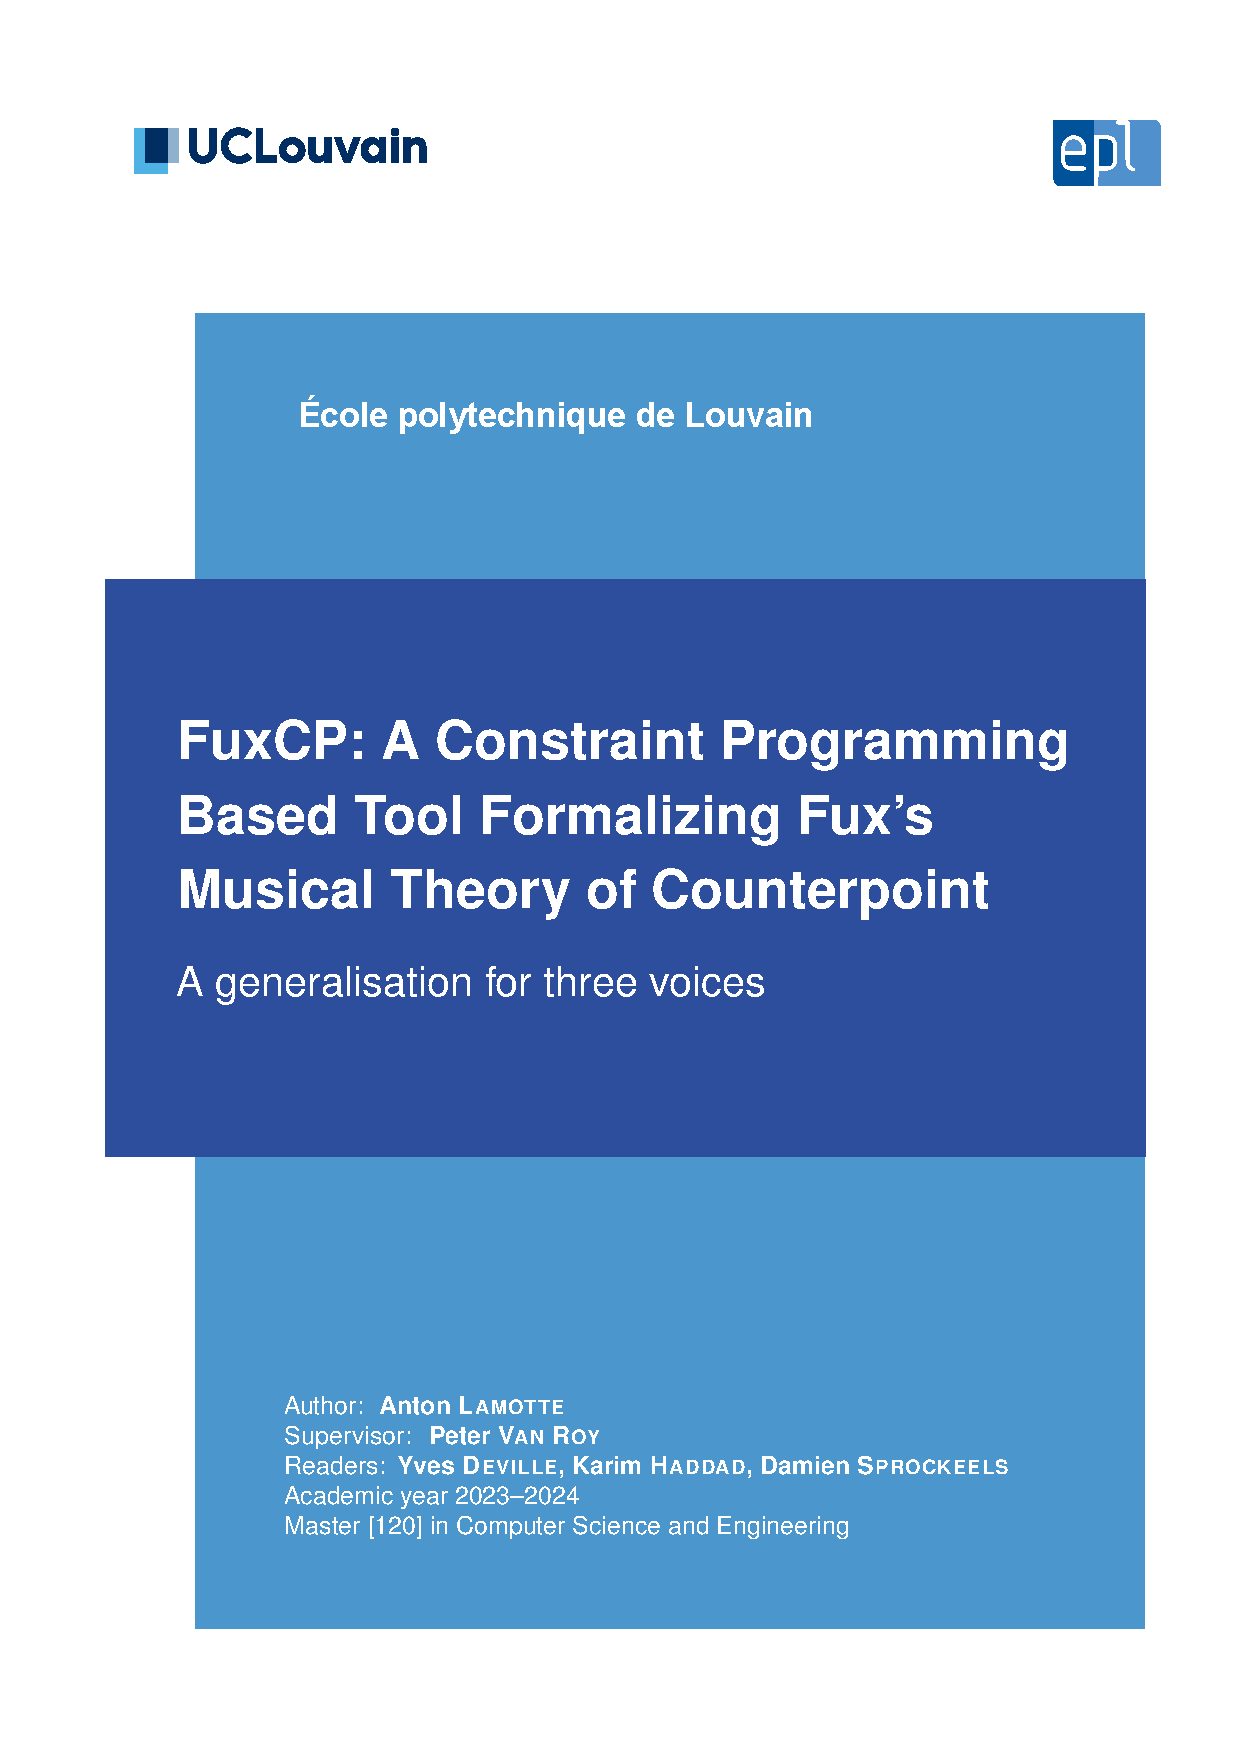
\includepdf[pages=1]{FrontPage.pdf}
%\null
%\thispagestyle{empty}
%\addtocounter{page}{-1}
%\newpage
%\newgeometry{left=1.65in,right=1.65in,top=2in,bottom=2in}
%\begin{abstract}
%    \large{
%        This master's thesis presents FuxCP, a tool for computer-aided contrapuntal composition. The objective is to assist composers without programming skills by automating repetitive and time-consuming tasks. The tool is based on constraint programming with Gecode and formalizes musical rules as constraints. Thanks to this approach, the tool provides transparency and control over the generated solutions, allowing composers to shape their desired music. This thesis focuses on formalizing the rules of two-voice counterpoint from Fux's \textit{Gradus ad Parnassum}. The research highlights the advantages of constraint programming over other approaches, as it allows the tool to "understand" the generated music. The thesis covers the formalization of counterpoint species-specific rules as mathematical constraints, the evaluation of the tool compared to Fux, and suggestions for future development. The conclusion emphasizes the importance of a comprehensive set of rules for formalization, the need for additional constraints on melodic development, and the potential for more expert solvers in other musical genres. The findings indicate the potential of constraint programming in enhancing computer-aided composition across various musical styles.
%    }
%\end{abstract}

%\chapter*{Acknowledgements}
%\paragraph{Thanks to Peter Van Roy}, my supervisor, for giving me the opportunity to write this thesis combining two of my passions: computer science and music.

%\paragraph{Thanks to Damien Sprockeels} for his pragmatic feedback, his devotion to the project, and his great contribution to computer music.

%\paragraph{Thanks to Karim Haddad} from IRCAM for proposing the \textit{Gradus ad Parnassum} as a reference book.

%\paragraph{Thanks to Yves Deville} for reading this thesis.

%\paragraph{Thanks to UCLouvain} for allowing me to finish my studies on such an instructive project.

%\paragraph{Thanks to Justine Nagant} for supporting me throughout this long ordeal.

%\paragraph{It is thanks to} the energy and time of all these people that this thesis exceeded my expectations.
%\restoregeometry

\tableofcontents

\chapter{Introduction and context of this work}
\pagenumbering{arabic}
This thesis is a formalisation of three-part counterpoint based on the writings and rules of Fux. Its aim is to provide a mathematical set of rules and a computer environment capable of translating Fux's teachings into formal logic, and capable of implementing these logical rules in a concrete way to produce Fux-style counterpoint.


This thesis will therefore be divided into several parts: we will first immerse ourselves in \gap, Fux's central work, from which we will meticulously extract the rules laid down by its author. We will briefly discuss these rules to make them unambiguous, and then translate them into formal logic, so that each rule Fux had in mind when writing his work is mathematically recorded. On this basis, we will create a computer implementation using constraint programming. We will then look at how this implementation finds results, discussing the search algorithm and heuristics used. We then discuss the cost techniques used to obtain the best possible results. Finally, we will analyse the musical compositions produced by the tool created.

It is very important to know that this thesis is based on T. Wafflard's thesis "FuxCP: a constraint programming based tool formalizing Fux's musical theory of counterpoint" \cite{wafflard2023} and article "A Constraint Formalization of Fux's Counterpoint" \cite{sprockeels2023constraint}. The present work takes up the concepts and definitions of T. Wafflard and could only be understood in its full depth by reading and fully understanding his works as well. A short summary is given in section \ref{section:thomas-in-a-nutshell}.



\section{A brief history of counterpoint: from the writings of Bach to algorithmic generation}
And before we get to the heart of the matter (which is the formalisation), let's take a look at Fux's theory of counterpoint, because that's the work that this work aims to formalise. Counterpoint is a compositional technique in which there are several musical lines (or voices) that are independent and distinct from one another but are balanced and sound beautiful \cite{CpSachs}. No voice is dominant over the others, and all are main voices, even though some may take a small precedence during part of the composition \cite{hess2016}.  


Counterpoint has been central to the work of many famous composers from different artistic movements, such as Bach in the Baroque, Mozart in the Classical and Beethoven in the Romantic \cite{kramer1987gradus}, has reached some modern music \cite{altozano2017contrapunto}, and has aroused interest over the centuries with the development of key texts on the subject, such as Schenker's Counterpoint \cite{schenker1906} or Jeppesen's Analysis \cite{jeppesen1960}. And while Bach was probably the master of counterpoint composition in his day \cite{yearsley2002}, the central and foundational work in the teaching of counterpoint belongs to another great Baroque composer: the Austrian Johann Joseph Fux and his treatise \gap. In it, this Baroque composer gives a detailed analysis of two-, three- and four-part counterpoint writing, all told as a discourse between a master and his pupil. \gaps was part of the species counterpoint movement, a way of conceiving counterpoint in five different types that could then be combined. It is on this work that this dissertation is based.


For Fux, but also for many other authors, species counterpoint are governed by many diverse rules, and it is these rules that interest us in the present work. The rules are based on old concepts that go back to older styles and have been discussed by many authors \cite{crocker1962}.  Those concepts include, for example, the notions of opposite motion and consonance (which in turn can be either perfect or imperfect). These concepts and their application to counterpoint are particularly interesting because they allow us to consider the composition of counterpoint both in a 'vertical' way, in which we consider the harmony of the notes played together, and in a 'horizontal' way, in which we consider the melodic development of each of the parts individually, which provides the independence of the counterpoints from each other and their melodic beauty.

This is what makes it interesting to analyse from a constraint programming point of view. We'll come back to this later, but for now let's concentrate on Fux's music theory.

\subsection{Fux's theory of counterpoint}
As we have just said, Fux uses a set of rules to create 'the right counterpoint'. These rules can be divided into three categories: melodic rules, harmonic rules and rules of motion. We will examine them here, bearing in mind that the formalisation of all the rules for two-voice counterpoint can be found in T. Wafflard's thesis, and that the complete set of rules (in mathematical form) can be found in the appendix \ref{appendix:complete-set-of-rule} to this thesis.

\subsubsection{Melodic Rules}

Fux explains that there are rules that apply within parts (the horizontal rules) about the order of the interval between one note and the next: we find, for example, that a melody is more beautiful\footnote{Throughout this work we will speak of the "beauty of music". This beauty is highly subjective, and therefore reference will be made to the Fuxian concept of music to define whether a melody is beautiful or not. In other words, music will be considered beautiful if it conforms to the rules of Fux, and vice versa} if the intervals between its successive notes are small, that there is no chromatic succession, if the notes that follow each other are varied, and so on. These 'horizontal' rules are called 'melodic' rules because they concern only the melody. These rules apply within a given counterpoint.


\subsubsection{Harmonic Rules}


If there is a horizontal perspective to counterpoint, there is also, of course, a vertical perspective. This perspective is expressed in a harmonic relationship between the different voices. At each point in the composition, a series of rules (known as 'harmonic rules' because they concern harmony alone) apply. For example, there is the rule that in the first beats of each measure the interval between the voices must be a consonance \footnote{A third, a fifth, a sixth or an octave.}; imperfect consonances\footnote{Thirds and sixths.} are preferred to fifths, which are preferred to octaves; and the rule that the different voices must be different at each point in the composition. These rules apply between the counterpoints.

\subsubsection{Motion rules}
Finally, there is a third type of rule: movement rules. These rules are a hybrid of the two discussed above in that they consider not only vertical interaction, i.e. harmony, but also horizontal interaction, i.e. melody. They can therefore be seen as 'diagonal' rules that relate the unique melody of each counterpoint to its respective harmonies. These rules include, for example, the fact that we prefer voices that move in opposite directions (i.e. if one voice goes up, we want the other to go down), the rule that there should be no sequence of fifths or octaves between voices, or the rule that we should not arrive at a perfect interval by direct motion.

\subsubsection{Preferences}\label{subsection:preferences-vs-hard-rules}
This last point does not really concern a kind of rule as such, but rather the preferences that Fux expresses in his work. These preferences are advice that Fux offers in order to write a nice counterpoint. As their name suggests, preferences are optional and not compulsory to follow, as other rules would be.

Fux is never clear about whether a rule\footnote{We use the generic term "rule" to refer to both mandatory rules and preferences.} is a preference or a strict rule --- and that's normal, what he conveys is mostly intuition, and human beings are quite capable of understanding whether a rule is a preference or an obligation; Fux probably didn't expect someone to try to formalise his work three centuries later.

These preferences should be respected whenever possible, and if not, so be it. Here's a good example: Fux indicates that we prefer to have as many different notes as possible in the composition. This is not an absolute rule, but a preference. The more variety there is in the composition, the more beautiful it will be, and the more preferable it will be.

\subsection{Species counterpoint}\label{section:species-counterpoint}
When we talk about species counterpoint, we're talking about five categories of counterpoint. Each species is a separate concept, each with its own peculiarities. We'll go into more detail about the different species below. Let's first concentrate on how species counterpoint works. When composing counterpoint, the starting point is a fixed melodic line, the \cf, which is a basic melody composed entirely of whole notes. It is the basis of a composition when writing counterpoint. It is from this voice and in relation to it that the others are composed. It is important to note that once the composition is complete, the \cfs is no more or less important than the other voices, and has the same melodic independence as the other voices. It is therefore nothing more than the basis from which we begin to write.

Let's take a look at the five species:
\begin{enumerate}
    \item \textbf{First species}: Note against note \textendash{} the counterpoint is composed entirely of whole notes, and the composition is a sequence of harmonies sounding on the first beat between the counterpoint and the other voices.
    \item \textbf{Second species}: Half notes against whole notes \textendash{} the counterpoint is composed entirely of half notes, which introduce dissonant harmonies.
    \item \textbf{Third species}: Quarters against whole notes \textendash{} the counterpoint is made up entirely of quarter notes, which allow more different movements and more freedom in the composition.
    \item \textbf{Fourth species}: The ligature \textendash{} the counterpoint is delayed by two beats, creating syncopation. The notes are all round (i.e., tied minims, since they span between two measures).
    \item \textbf{Fifth species}: Florid counterpoint \textendash{} counterpoint is a mixture of all the other species and is the richest form of counterpoint. It allows great freedom of composition while respecting the rules of the other types.
\end{enumerate}

Although these types could technically be combined to form a three-part composition with two different types of counterpoint, Fux seems to prefer to write a 'special' counterpoint (i.e. second, third, fourth or fifth species) in one voice and only whole notes (i.e. a first species counterpoint) in another voice. He also sometimes says that it is possible and recommended to mix species, but does not do so extensively.

\subsection{Building a computer tool for writing species counterpoint}
We've just explored the longstanding tradition of counterpoint, a musical style shaped by countless generations of composers. As technology advanced, the idea of automating counterpoint composition emerged. An early attempt, by Schottstaedt in 1984 \cite{bill1984}, involved an expert system based on Fux's rules. His approach used over 300 if-else clauses, but this method had obvious limitations compared to what modern constraints are capable of.

Indeed, it's crucial to understand that if-else clauses are unidirectional, whereas constraints are bidirectional. Schottstaedt's algorithm relied heavily on specific conditions, captured by numerous if-else clauses. In contrast, modern constraint systems support bidirectional constraints with multiple arguments. These systems don't just find single solutions, they represent sets of potential solutions. This flexibility is a significant improvement over the directional nature of if-else clauses.

Furthermore, constraint systems offer an advantage in specifying intricate search heuristics. This adaptability and efficiency highlight the stark contrast between the outdated approach of if-else clauses and the modern capabilities of bidirectional constraint systems in the realm of counterpoint composition.

\paragraph{}
In 1997, a genetic programming and symbiosis approach to automatic counterpoint generation was developed. A team from Michigan used this approach to optimise counterpoints of the 5th species and make them more attractive \cite{polito1997musica}. A similar approach was used in 2004 to generate fugues (hence counterpoint), also using genetic algorithms \cite{garay2004fugue}. The results are quite promising, and generate more than interesting results, but the end result is still far from being able to provide a complete counterpoint composition.

Many years later, in 2010, a team of researchers from the University of Malaga developed an automated method for the generation of first-species counterpoint using probabilistic logic \cite{Aguilera2010}. Their approach was specifically tailored to compositions in C major, providing a generated counterpoint in response to a given \cf. Please note that this application only evaluates the harmonic attributes of the counterpoint, ignoring the melodic aspect.

Two years later, a team from London developed a way to generate high-quality first-species counterpoint using a variable neighbourhood search algorithm \cite{Herremans2012}. Their research was limited to first-species counterpoint, but they addressed issues such as preferences (finding the best counterpoint) and user-friendly interface. Once again, their results are more than impressive, but their research is limited to the first two-voice species.

Finally, a research was carried out in 2015 on Fux's counterpoint \cite{komosinski2015automatic}, with the aim of generating the first species counterpoint using dominance relations, has yielded fairly good results. The search demonstrates the use of this paradigm and its applicability, and is a good starting point for composing counterpoints of other species based on the same concept.

\paragraph{}
If we now focus on applications that have gone as far as the user interface and are now ready to be used, we should mention two namesakes, both called 'Counterpointer', which have the merit of offering a functional tool for composing counterpoint.

The first Counterpointer tool \cite{counterpointer_ms}, which anyone\footnote{Anyone... or almost, as it is a paid tool.} can use to check the validity (or not) of their counterpoint. Its last release was in 2019 as a desktop application, and it works like this: an apprentice composer tries to write a counterpoint, and then submits it to the tool. The tool then decides whether the counterpoint is valid according to the traditional rules of counterpoint\footnote{Not only Fux's rules, but also those of other authors.}. It also provides feedback to help the student composer improve their future counterpoint writing. The tool is not able to write counterpoints automatically, nor is it explicit about how it works, as it is completely closed source and has no accessible report. It is therefore impossible to know the paradigm it uses or the exact rules it follows.

Another attempt at automatic counterpoint writing is the Counterpointer project in 2021, created by a team of students at Brown University as part of a software engineering course \cite{counterpointer_project}. The project is less accomplished than the aforementioned application, but it has the merit of being able to generate two-voice counterpoints of the first, second and third species. It is an entirely free and open source project. While the results are encouraging, the project has been discontinued as it was a course project and their method of finding a counterpoint seems much less efficient than the efficiency that a constraint solver can achieve. 


\paragraph{}
This brief overview leads us to conclude that there is no satisfactory tool for composing counterpoint in a user-friendly way, with good quality, quickly and with several voices. It is to fill this gap that this research has been carried out. This was the aim of T. Wafflard's thesis and it is therefore natural that this thesis should follow in his footsteps.



\section{Standing on the shoulders of giants: underlying works and editions of \gaps used}
As has just been said, this work is the continuation of T. Wafflard's work. However, it also relies heavily on the work of
\begin{itemize}
    \item \textcite{GiLthesis}, who presented an interface for using Gecode functions in Lisp called "GiL". This interface was then tested with some rhythm-oriented constraints.
    \item \textcite{Melothesis}, who explored the use of constraint programming in OpenMusic using GiL. The tool that was produced in this thesis is capable of producing songs with basic harmonic and melodic constraints.
    \item \textcite{Melo2thesis}, who created a tool capable of combining the strengths of the first two implementations while continuing to develop support for GiL.
\end{itemize}

As with T. Wafflard, the musical reference work chosen is Fux's \gap, because it is a pillar of counterpoint theory and because it is fairly easy to extract rules from it (although Fux is sometimes very vague about his intentions). And as with any book published several centuries ago (1725 in the case of \gap), there are many versions and translations. This is good news, as Fux can sometimes be really unclear about what he means, and having many versions (some annotated, some not) from many people who also had to interpret Fux to translate it is a great treasure, as it helps to clarify Fux's meanings. This work is therefore based on several different editions and translations of the book, although it is mainly based on Alfred Mann's English translation \cite{GaPEng}. French (both Chevalier's \cite{GaPFrChevalier} and Denis's \cite{GaPFrDenis}), German \cite{GaPDe} and Latin \cite{GapLa} translations are used when it is necessary to remove an ambiguity or clarify an unclear rule. These translations have been chosen because French is the \textit{lingua franca} of the team; German is the language of Fux and the environment in which he developed; and Latin is the original version, so we can hope that it is the most faithful to what he wanted to convey.

\section{Tools and implementation}\label{subsection:tools-and-implementation}
This subsection discusses the implementation of the automatic counterpoint generator. To do so, we briefly explain how constraint programming works, the tools used by FuxCP, and the actual implementation of it.

\subsection{Constraint Programming}
Constraint Programming (CP) is a programming paradigm used to solve large combinatorial problems, such as planning and scheduling problems. It works by defining constraints between variables that limit the values these variables can potentially take \cite{rossi2008constraint}. In doing so, the domains of these variables are reduced. R. Barták explains in a very clear way what a constraint really is, as he describes in his "Guide to Constraint Programming" \cite{bartak1998constraint}:

\begin{quote}
    A constraint is simply a logical relation among several unknowns (or variables), each taking a value in a given domain. A constraint thus restricts the possible values that variables can take, it represents some partial information about the variables of interest. For instance, "the circle is inside the square" relates two objects without precisely specifying their positions, i.e., their coordinates. Now, one may move the square or the circle and he or she is still able to maintain the relation between these two objects. Also, one may want to add other object, say triangle, and introduce another constraint, say "square is to the left of the triangle". From the user (human) point of view, everything remains absolutely transparent.
\end{quote}

\paragraph{Constraint propagation}
Each time a constraint is defined, the domain of the affected variables is reduced according to the possibilities left by the constraint. This is called constraint propagation. Let's imagine a variable $A$ whose domain is $\{0, 1, 2, 3\}$ and a variable $B$ whose domain is $\{0, 1, 2\}$. When the constraint $A<B$ is applied, the domain of $A$ is reduced to $\{0, 1\}$, because the new constraint makes it impossible for $A$ to have a value of $2$ or $3$ without violating the constraint.

A constraint solver is an implementation that systematically browses the search space in look for a solution. A given problem can have many solutions, just one, or even none, if the domains are too small or the constraints contradict each other, and the system becomes overconstrained.
A solution is found when all variables are fixed, i.e. their domain is reduced to a single value. We know that a problem has no solution if a domain is empty after a constraint has been declared (because this means that no value can be found for that variable that does not violate the constraint).

\paragraph{Branching}
Obviously, declaring constraints is not enough to magically find a solution. In the example we proposed earlier (with A and B), the single constraint placed on the search space doesn't allow us to determine the values of A or B, and their domains remain composed of more than one value. 
To actually find a solution, the constraint performs a branching. That is, it studies two antagonic possibilities and splits the search space into two subproblems accordingly. More specifically, it chooses a variable and studies the case where that variable is equal to a certain value, and the case where it is not equal to that value. For example, the solver might study the case where $B=0$ (the first branch) and the case where $B \neq 0$ (the second branch). If the solver finds an inconsistency in either case, it knows that the entire branch can be discarded (as it does not lead to a valid solution). Immediately after branching, the solver again performs constraint propagation, since constraint propagation occurs whenever any domain is modified, and consists of adjusting all domains to which the modified domain is linked by a constraint. In our case, after setting $B$ to $0$, the solver propagates all constraints linked to $B$, i.e. the only constraint in our problem (i.e. $A<B$). This affects the domain of $A$, reducing it to an empty domain (because no value in the domain of $A$ is less than $0$). The solver, noticing that one domain is empty, concludes that this branch contains no solution and therefore knows that the only possible branch is the other one, i.e. the one in which we assumed $B\neq 0$. We can therefore safely remove $0$ from the domain of $B$, since this value is not contained in any solution. Repeating the branching process each time it is necessary produces three solutions: $A=0$ and $B=1$, $A=0$ and $B=2$, and finally $A=1$ and $B=2$.

\paragraph{Heuristics}
As with all problems involving searching a space in quest of a solution, it is very useful to have heuristics allowing for an efficient search. A heuristic is a rule or strategy used to make informed decisions about variable assignments and value choices during the solution search. These rules are designed to exploit the characteristics and structures of the problem to improve the chances of finding solutions more quickly. A common heuristic is variable ordering, where the algorithm selects variables to assign values to based on factors such as the size of the domain or the number of associated constraints. Another important heuristic is value ordering, which determines the order in which values are tested for a given variable assignment. By incorporating heuristics, constraint solvers can prioritise the most promising branches of the search tree, effectively reducing the search space and speeding up the identification of feasible solutions. While heuristics speed up the solving process, it's important to strike a balance between exploration and exploitation, as overly aggressive heuristics risk missing potentially valuable solution paths.


To return to our previous example, a value-ordering heuristic might be "branch first on low values of $A$ and high values of $B$, since we know that we are looking for a solution where $A$ is less than $B$, and we can reason that there are more chances of satisfying this constraint when $B$ is large and $A$ is small.

\paragraph{Costs in Constraint Programming}
While the basis of Constraint Programming is this succession of propagations and branchings, there also exists a notion of cost, which distinguishes between two valid solutions (i.e. satisfying all constraints) into a less good solution and a better solution.


For example, in our simple example, we could define cost as the sum of $A$ and $B$ and want to minimise the cost. This means that we are looking for a valid solution where $A$ and $B$ are as small as possible. In this case, only the first of the three solutions mentioned above is chosen, i.e. $A=0$ and $B=1$, as it is the best possible solution (with a cost of 1).

\paragraph{Branch and Bound}
Branch and Bound is a systematic algorithm used in Constraint Programming to efficiently explore the solution space and find an optimal solution with respect to a given cost or objective function. This technique extends the basic Constraint Programming approach by introducing a mechanism to prune unpromising branches of the search tree, thereby reducing the computational effort required to find the optimal solution. The algorithm starts with the initial problem and iteratively divides it into subproblems, called branches, by making decisions about variable assignments. For each branch, the algorithm evaluates its feasibility and its potential to lead to a better solution. If a branch is deemed infeasible or cannot possibly improve on the current best-known solution, it is pruned from further consideration. This process continues until all branches have been explored, or until the algorithm converges on the optimal solution. Branch and Bound is particularly valuable for large combinatorial problems because it efficiently narrows the search space, allowing the solver to focus on promising regions and accelerating the discovery of optimal solutions in constrained programming scenarios \cite{morrison2016branch}. 

\subsubsection{Relevance of the use of constraint programming in the field of music}
The question now is: what is the connection between this problem-solving method and counterpoint composition? Well, it turns out that music is actually a very good application of constraint programming: you can represent all aspects of a composition by variables, set rules between these variables, and the solver takes care of finding a valid solution. In fact, in music, it's never just one factor that determines whether the music is beautiful, but an interaction of many. And as humans, it's sometimes difficult to find a valid solution (i.e. to compose music that sounds good) because the range of possibilities and the interactions between factors are so numerous.  However, as we have just seen, exploring a search space in which a large number of constraints are defined is something that a constraint solver does very well. The most arduous task then becomes putting the rules that make music beautiful down on paper, and this is the task that many musicologists and composers have set themselves. Once these rules have been defined by musicologists and composers, it is "simply" a matter of formalising them and passing them to the constraint solver so that it can compose a melody that respects these rules.

What's more, by defining a rigorous way of distinguishing a good composition from a bad one, the solver can even find increasingly beautiful solutions.

\subsection{Open Music}
OpenMusic is a powerful and innovative visual programming environment, written in CommonLisp, designed specifically for composers, researchers and musicians involved in computer-aided composition \cite{OpenMusic}. Developed by the Institute for Research and Coordination in Acoustics/Music (IRCAM) in Paris, OpenMusic provides a graphical interface that allows users to create and manipulate musical structures using a variety of predefined modules. This visual programming language facilitates the representation of complex musical ideas, algorithms and data flows through a user-friendly interface, making it accessible to both novice and experienced composers. 


FuxCP is a library for OpenMusic, which means that OpenMusic is the interface for using FuxCP. Any user wishing to use FuxCP writes their \cfs (FuxCP's input) into OpenMusic and then launches the solution search from within OpenMusic. Specifically, FuxCP retrieves the \cfs from OpenMusic and then defines the constraint problem. When a solution is found, it is passed to OpenMusic and the user gets it as an OpenMusic object.

\subsection{Gecode and GiL}
After receiving the input (which is the \cf), FuxCP uses Gecode to define the search space and starts searching for a solution. Gecode, short for Generic Constraint Development Environment, is an open source toolkit for developing constraint-based systems \cite{Gecode}. It provides a high-level C++ library for efficiently modelling and solving constraint problems. Gecode supports a wide range of constraints, variables, and search strategies, making it a versatile platform for tackling combinatorial problems such as scheduling, optimisation, and configuration. 


Since FuxCP is an OpenMusic library written in Lisp, it is naturally written in Lisp too. To be able to use the Gecode C++ library, FuxCP uses the Gecode Interface Lisp (GiL), which is a wrapper that allows Gecode functions to be used in Lisp programs. It in turn relies on The Common Foreign Function Interface (CFFI), which is an interface for calling C++ functions in Lisp \cite{CFFI}.  GiL is far from complete, but it provides enough tools to solve interesting constraint problems in Common Lisp.

\subsection{Concrete implementation}
To put it all together: FuxCP gets its input (the \cf) from the user interface, which is OpenMusic. It then defines a constraint programming problem in Gecode, using GiL. 

As for the way it defines the problem, here is a little clarification: first, when the \cfs is received, a whole series of constants and variables are defined: for example, the length of the \cf, the arrays representing the pitches of the counterpoints, ...
Then all these variables are constrained according to the constraints defined in the formalisation of Fux's rules (discussed in chapter \ref{chapter:species}). The constraints are set sequentially: first the constraints on the \cf, then the constraints on the first counterpoint, and finally the constraints on the second counterpoint. A diagram of the code architecture and the integration of FuxCP with other tools can be found in Appendix \ref{fig:softwarearchitecure}.


\section{T. Wafflard's thesis in a nutshell}\label{section:thomas-in-a-nutshell}

In 2023, T. Wafflard proposed a complete formalisation of Fux's two-voice counterpoint \cite{wafflard2023}. This formalisation takes each of the rules given by Fux about two-voice composition and translates them into formal logic. Those formal relations are then translated into constraints and given to a constraint solver. When given an input \cf, the solver applies all the constraints it was given and yields an output counterpoint. The following subsection is not intended to be an exhaustive summary of all of T. Wafflard's excellent work, but rather a brief outline of the idea behind it and the procedure followed. This brief overview is given to the reader because many of the concepts in T. Wafflard's work are at the heart of the three-voice generalisation and will be key to understanding the three-voice formalisation.

\subsection{Variables} \label{Wafflard-variables}
In order to formalise Fux's rules, it was necessary to define variables whose purpose is to represent a compositional reality. Thus T. Wafflard created variables to represent various concepts, such as the pitch of notes (written $N$), the harmonic interval between voices (written $H$), the melodic interval from one note to the next (written $M$), and many others. These variables are then related to each other according to the formalised rules. The constraint solver searches for all possible values of these variables, according to the constraints, and stops when all variables in $N$ (the pitches) are fixed, as this means that a solution has been reached (the notes of the counterpoint are known, and this is the goal of the solver).

Useful constants were also defined and will be reused throughout this work. The most important of these are $m$, which represents the length of the \cfs (and thus the number of bars in the composition), $n$, which represents the number of notes in a given counterpoint, or Cons$_{\text{all, p, imp}}$, which represents the set of consonances (all, perfect and imperfect).

Of course, there are many different solutions for the same \cf, and in order to distinguish between two valid solutions (i.e. all solutions that respect all constraints), some costs have been defined. These costs are intended to convey the preferences expressed by Fux in \gap. In fact, Fux sometimes expresses a preference that is not an absolute rule: "this should be done if possible, but is not necessary". Thus, the solver considers a valid solution with a low cost to be better than a valid solution with a high cost. The costs scale from 0 (when we don't care) to 64$m$ (when something should only happen as a last resort), but most costs scale from 0 to 8. These costs are then added together to form a total cost, which the solver tries to minimise.

\subsection{Array notation}
As we have just seen it is necessary to refer to numerous arrays, that formally represent the musical composition and many of its underlying aspects (pitches, harmony, melody, ...). These arrays always have two indexes: the first index represents the time in question, the second index represents the measure in question. These indices are written in computer notation. For example, $X[3, 7]$ represents the variable $X$ on the 3rd beat of the 7th measure.

Let's put it all together. Here is a simple example of how the variables and constants are brought together through the formalisation: 
\begin{equation}    
    H[0, m] \in Cons_{\text{perf}}
\end{equation}
 This is a rule which means that the last harmonic interval must be a perfect consonance\footnote{Please refer to section \ref{subsection:modified_variables} for more exact details}. All rules from T. Wafflard's thesis can be found in appendix \ref{appendix:complete-set-of-rule}.

 \subsection{In practice}
 In practice, to solve this constraint programming problem, the constraints are written in Lisp, and thanks to the Gecode Interface Lisp (GiL) \cite{GiL}, it uses the Gecode constraint solver \cite{Gecode} to find a solution. To make the constraints work, we need a starting point. The starting point is the \cf (see \ref{section:species-counterpoint}).
 When given a \cf, the solver defines a set of variables (those mentioned in the formalisation) to which constraints are then applied (the relations from the formalisation) and produces a counterpoint that obeys all the rules that have been defined and whose quality can be given by the cost. As explained in \ref{Wafflard-variables}, in the case of T. Wafflard's implementation, the total cost is the sum of all the costs, and this cost is minimised by a depth first search algorithm that finds the lowest cost, and then gives the corresponding solution.
 
 
 As for the front-end, all the user sees and interacts with is OpenMusic \cite{OpenMusic}, an object-oriented visual programming environment for musical composition based on Common Lisp \cite{commonlisp} developed by the Parisian institute IRCAM (Institute for Acoustic/Music Research and Coordination) \cite{IRCAM}.
 
 The present work has exactly the same basic functioning (as is explained in the previous subsection \ref{subsection:tools-and-implementation}). 


\section{The contributions of this thesis}
The aim of this work is to generalise T. Wafflard's formalisation to three-voice counterpoint, still based on Fux's work, and to create the corresponding implementation. It would be too easy to believe (wrongly) that three-voice counterpoint is nothing more than the combination of two two-voice counterpoints. From this point of view, we would then calculate a first counterpoint according to the \cf, and then a second counterpoint again according to the \cf, and that's it. Obviously, this view is too simplistic and doesn't really capture all the interactions between three voices. It is to this point (the peculiarities brought about by the addition of a third voice) that a whole chapter of this thesis is devoted. Another chapter is devoted to translating the rules from \gap into formal logic. A final but not less important section discusses and analysing the impact of costs, and the musicality of the solutions. The following is a more detailed summary of the contributions of this thesis. 
\begin{itemize}
    \item \textbf{Introducing new concepts and redefining variables}:
    As we have just mentioned, a three-part composition is much more than a (two+one) part composition. So we had to redefine and define a whole series of concepts to adapt to this reality. The creation of the (lowest, middle and highest) stratum concept is part of this, and is essential for formalising Fux's counterpoint constraints. All of this is discussed in Chapter \ref{chapter:defining-some-concepts-and-redifing-the-variables}.
    \item \textbf{Mathematical formalisation of three-part counterpoint}: As with the two parts of the formalisation, we rewrote Fux's explanations into unambiguous English and then translated them into logical notation. This formalisation builds on the previous formalisation for two voices, and sometimes (rarely) has to modify it. This formalisation can be found in Chapter \ref{chapter:species}.
    \item \textbf{Implementation of a working constraint solver for a three-voice composition}: Those logical rules were then implemented as constraints and the solver was adapted to allow a search for two counterpoints. The whole code of this implementation can be found in Appendix \ref{chapter:whole-code}, and its architecture in the Appendix \ref{chapter:architecture}.
    \item \textbf{Researching the best way to express Fux's preferences}: Three-part composition introduces so many possibilities for result composition that it is important to rethink the way we think about preferences. These preferences are understood by the solvers as costs (where a preferred solution in Fux's sense has a lower cost to the solver). Therefore, some techniques for managing these preferences are discussed to find out the best way to implement them as costs. This is very important as it allows the solver to produce solutions with high musicality. These techniques are discussed in Chapter \ref{chapter:search}
    \item \textbf{Musical analysis of the solutions generated by the solver}: Finding the best solution also means being able to assess the quality of current solutions. For this, see Chapter \ref{chapter:musicality}. 
    \item \textbf{Adapted user interface to allow them to compose with three voices and set a cost order}: All the new capabilities of the solver and the costing techniques must also be accessible to the user: it is now possible for a user to freely combine any number of species to form a three-part composition, and to set a cost order to indicate their preferences to the solver (in addition to the previous ability to set personalised costs). A guide for this can be found in Appendix \ref{chapter:user-guide}.
\end{itemize}
% citer Fux page 71 
\chapter{Defining some concepts and redefining the variables} 
\section{Voices, parts and strata}\label{section:parts-and-strata}
Before we start this section, we need to look at some vocabulary to make sure we understand what we are discussing. The most important definition (and distinction) we will introduce is the definition of the terms \textit{part} and \textit{stratum}. The need for these definitions arises from the increasing complexity of the rules of counterpoint when it is generalised to three voices. Indeed, the rules are no longer (as we shall see later) concerned solely with counterpoint and its cantus firmus, but also with new concepts, such as that referred to by Fux as 'the lowest voice'. As the term 'voice' is too generic (it is used in Fux's text to describe notions as different as counterpoint, cantus firmus, voice range and the so called 'lowest voice'), we need to create a precise vocabulary that is different from the word 'voice' to talk about these new concepts. 

With this in mind, let's explain what 'parts' and 'strata' are. Each of these two concepts is a type of voice, which means that in a composition with $n$ voices, there will also be $n$ parts and $n$ strata.

\subsubsection{Parts}
The parts correspond to what a given individual sing. They correspond to a staff (each staff corresponds to one part). The term 'part' is the same as that used by Fux in his work. The three parts in a three voices composition are: the \cf, the first \cp and the second \cp. Fux differentiates them by calling them by the name of their voice range, that is: "bass", "tenor", "alto" or "soprano".

\subsubsection{Strata}
As for the strata, they are defined like this: a stratum delineates discrete layers or levels of pitches at any given moment in the composition. It denotes a vertical alignment of simultaneous notes and organizes them into distinct strata. By definition, the lowest stratum encompasses the lowest sounding notes, the highest stratum comprises the highest sounding notes, and intermediary strata represent pitch levels in between.
This concept is very helpful in identifying and categorising the vertical placement of pitches, creating distinct categories of sound within the overall texture of the counterpoint composition. It provides a way of analysing and understanding the distribution of pitches across different parts, allowing more complex rules to be established: for example, it would now be possible to establish a rule between the notes of the cantus firmus and the highest sounding notes (no matter which part they come from). The full potential of strata lies in harmonic rules, but as we shall see, some melodic rules are also related to it.

\begin{minipage}{0.6\textwidth}
    The term stratum was chosen in this context for its visual impact. In geology, a stratum "is a rock layer with a lithology (texture, colour, grain size, composition, fossils, etc.) different from the adjacent ones", see figure \ref{fig:geological-strata}.
    \end{minipage}
    \hfill
    \begin{minipage}{0.3\textwidth}
      \centering
      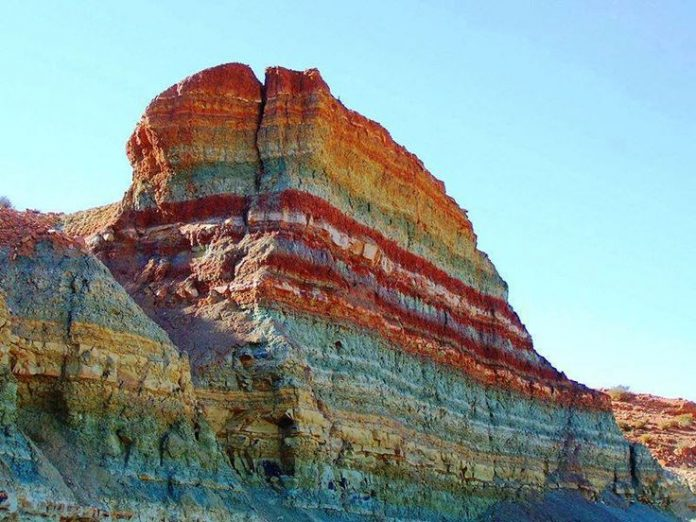
\includegraphics[width=\textwidth]{Images/rainbow-sediment.jpg}
      \captionof{figure}{Geological strata, for the illustration}
      \label{fig:geological-strata}
\end{minipage}
\vspace{.5cm}

When Fux speaks about the lowest stratum, he often uses the word 'bass'. It was deliberately chosen to speak about the 'lowest stratum' instead of the 'bass' (like Fux does), because 'bass' is also the name of a range of voices (on a par with soprano and alto, for example), and there is already enough complexity in all the terminology to add even further ambiguity. 

\paragraph{}
These new terms (parts and strata) are used where the distinction between the concepts is important. Whenever this distinction is not relevant, the more general term 'voice' is used to reduce the complexity of reading. In this case, the 'voice' could refer to both a stratum and a part.

Since a picture is worth a thousand words, Figure \ref{fig:lowest} illustrates the difference between parts (the blue lines) and strata (the red and orange lines). The lowest stratum is shown in its own colour (red) because it is the most meaningfull stratum, and it will be particularly important later on.

\begin{figure}[h]
  \centering
  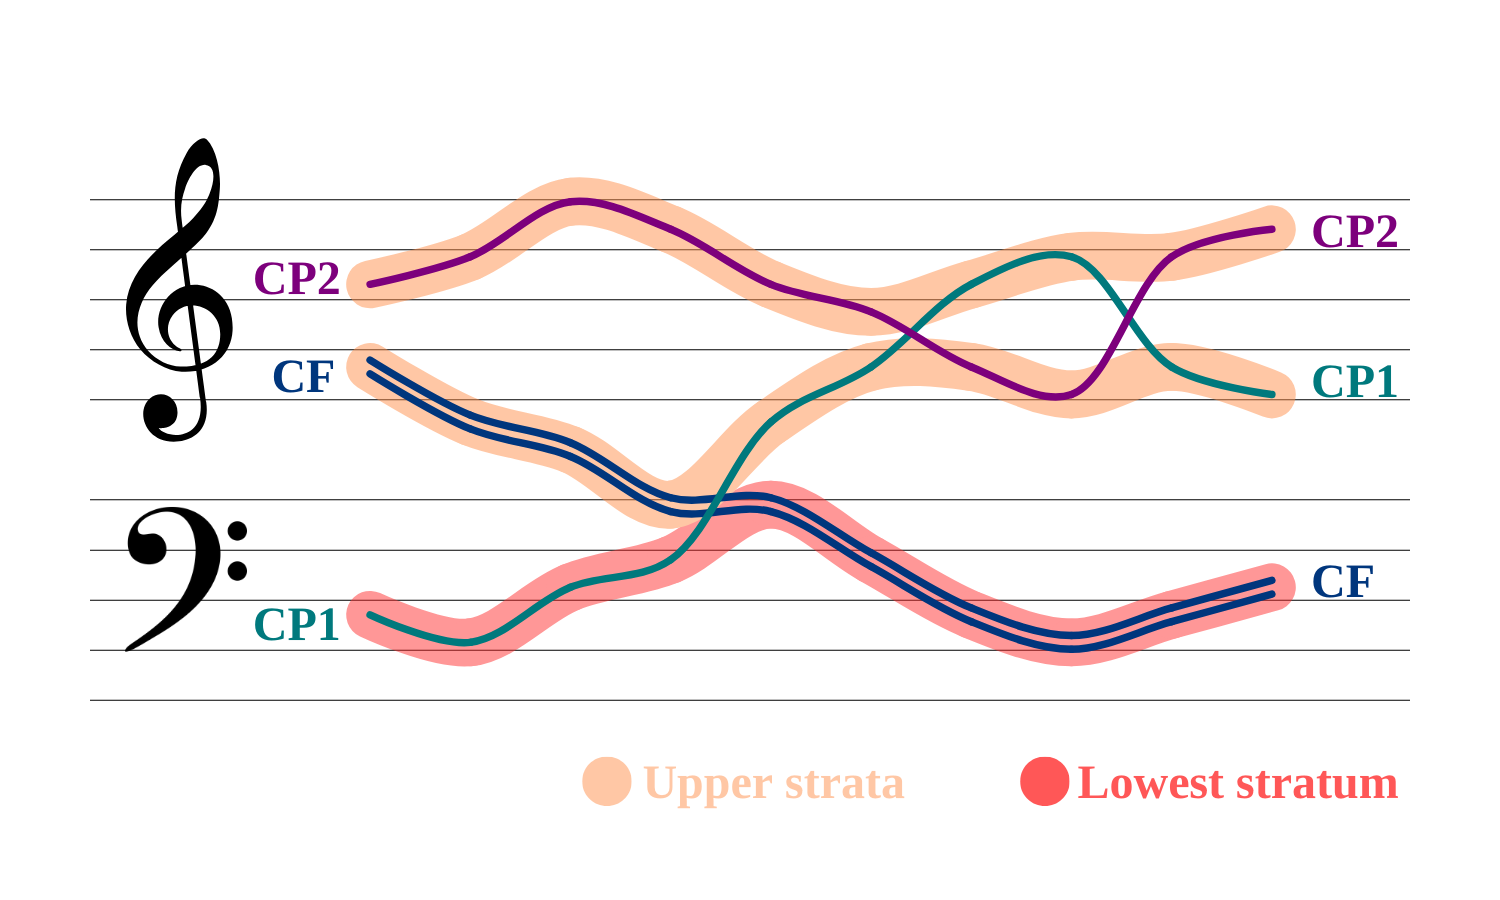
\includegraphics[width=1\textwidth]{Images/strata_example.png}
  \caption{Parts and strata in a three voice composition}
  \label{fig:lowest}
\end{figure}


Here is also the mathematical representation for the notes of the lowest stratum (written $N(a)$, see section \ref{section:changes induced} for the notations):
% todo a, b, c, et A
\begin{equation}
    \forall i \in [0, 3] \quad \forall j \in [0, m-1): N(a)[i,j] = \text{max} (N(cf)[i,j], N(cp_1)[i,j], N(cp_2)[i,j])
\end{equation}

Of the first upper stratum, or medium stratum (written $N(b)$, see section \ref{section:changes induced} for the notations):
\begin{equation}
    \forall i \in [0, 3] \quad \forall j \in [0, m-1): N(a)[i,j] = \text{med} (N(cf)[i,j], N(cp_1)[i,j], N(cp_2)[i,j])
\end{equation}

And of the second upper stratum, or uppest stratum (written $N(c)$, see section \ref{section:changes induced} for the notations):
\begin{equation}
    \forall i \in [0, 3] \quad \forall j \in [0, m-1): N(a)[i,j] = \text{min} (N(cf)[i,j], N(cp_1)[i,j], N(cp_2)[i,j])
\end{equation}

\subsubsection{One part per stratum and one stratum per part} \label{subsubsection:one-part-per-stratum}
It is important to note that, for each musical measure, there is a bijection between the individual parts and the corresponding strata. This means that, for any given measure, each stratum uniquely corresponds to a single part, and vice versa. Put differently, if two parts within a measure share the same pitch, they do not constitute the same stratum. Instead, one part corresponds with one stratum, and the other one to a separate stratum.

To illustrate this, consider a scenario in a two-voice composition (see figure \ref{fig:one-voice-max-can-be-a}), where part 'cf' and part 'cp1' in measure X both have a pitch value of 67 (representing a G). Despite having identical pitches at the same moment, one part is categorised as the lowest stratum, while the other is designated as the uppermost stratum. This distinction becomes crucial for subsequent analysis, especially when calculating aspects like motions.

To know which part gets to be the lowest stratum in such situations, an arbitrary hierarchical rule is implemented. If the ambivalence is between the \cfs and another part, the \cfs is always prioritised and assigned the role of the lowest stratum, over any other part. In the case of a ambivalence between the first \cp and the second \cp, the first \cp is given the status of the lowest stratum. 

\begin{figure}[h]
    \centering
    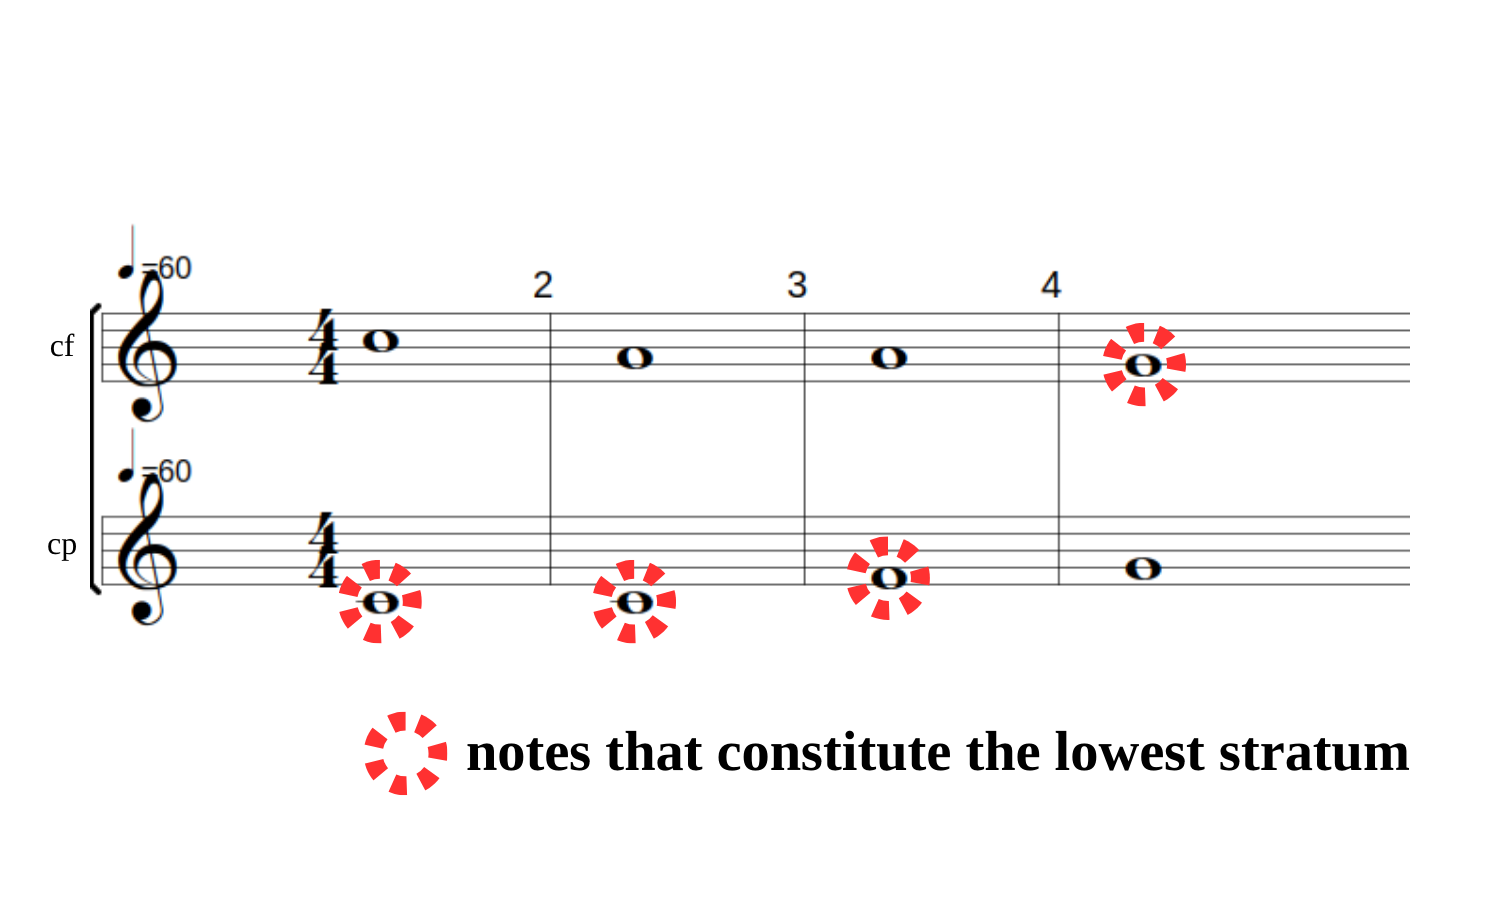
\includegraphics[width=.5\textwidth]{Images/one-voice-max-can-be-a.png}
    \caption{Establishing which part corresponds to the lowest stratum}
    \label{fig:one-voice-max-can-be-a}
  \end{figure}

\section{Exploring the interaction of the parts with the lowest stratum}

One of the major differences between the composition of two voices (i.e., one \cfs and one counterpoint) and the generalisation to three voices (i.e., one \cfs and two counterpoints) is that the rules no longer necessarily apply between the counterpoints and the \cf. If we go back to the rules for two voices, we see that each of them applied between the single counterpoint and the \cf. For example, when it was stated that each interval must be consonant, this referred to the interval between the counterpoint and the \cf.
On the other hand, in his second part (where he describes the rules for composing in three voices), Fux explains that the rules are not necessarily to be observed between each of the counterpoints and the \cf, but rather between "each of the voices and the lowest voice" (i.e. the lowest stratum). Again, if we take the example of the need for consonance between the voices, consonance will be required in the intervals between the notes of any voice and those of the lowest voice (whether or not the latter is the \cf).
Fux approaches the concept of lowest stratum without ever stating it clearly, mentioning for example that the lowest voice can change (sometimes the bass is the lowest voice, sometimes the tenor, ...), and that at any given moment the lowest voice should be considered. In other words, Fux says that the rules apply between the parts and the lowest stratum.

\paragraph{}
One might be tempted to conclude that three-part composition breaks completely with two-part composition, but that would be too hasty a conclusion. Indeed, on closer inspection, the way the rules worked in two-part composition (from counterpoint to \textit{cantus firmus}) is just one particular case of this new vision of things. In two-part composition, too, the rules apply between the parts and the lowest stratum. But of course, since there were only two voices, the lowest stratum was either counterpoint or cantus firmus. This means that when links were established between the upper part and the lowest stratum, links were also established between the counterpoint and the cantus firmus. Considering the rules as being established between the counterpoint and the \cfs was just a simplification of reality, although it was perfectly correct. We were therefore considering a convenient particular case, and not the general case. Please note that when we talk about "applying constraints from voice A to voice B", it is clear that the constraints are bidirectional and that they also apply from voice B to voice A. What is shown here is rather the philosophy behind the application of these constraints, and the reasons why they were imposed.

The particular case happening when composing with two parts is illustrated in figures \ref{fig:cp2cf-2v} and \ref{fig:p2l-2v}. As we can see on those pseudo-compositions, it does not change anything to apply the constraints from the counterpoints to the \cfs or from the parts to the lowest stratum.

\vspace{.5cm}
\begin{minipage}{0.46\textwidth}
    \centering
    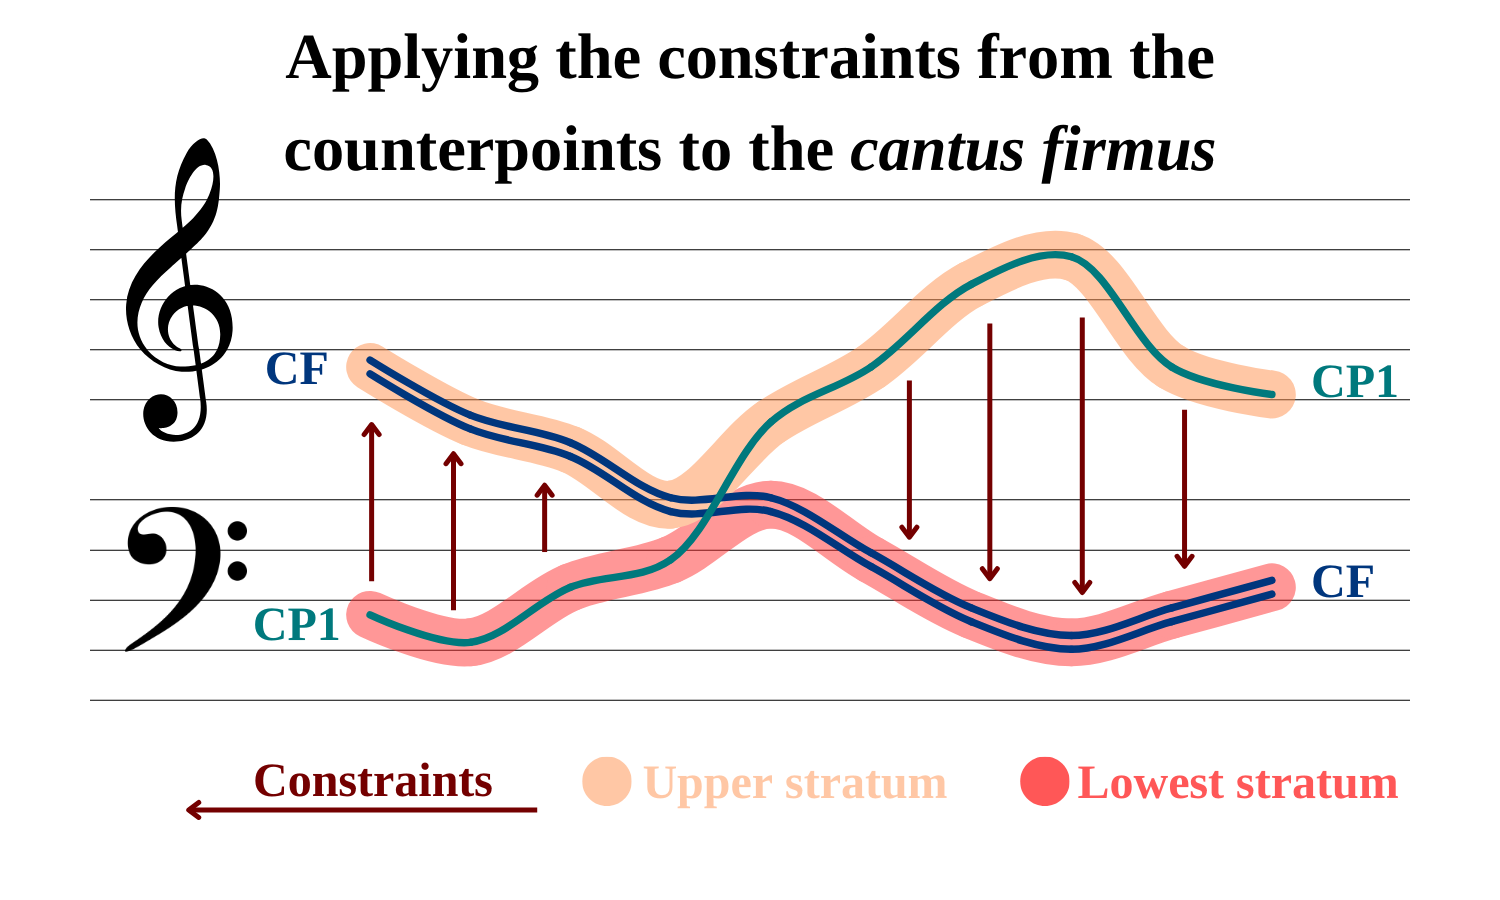
\includegraphics[width=\textwidth]{Images/cp2cf-2v.png}
    \captionof{figure}{Applying the constraints from the ctp. to the \cf}
    \label{fig:cp2cf-2v}
    \end{minipage}
    \hfill
    \begin{minipage}{0.46\textwidth}
      \centering
      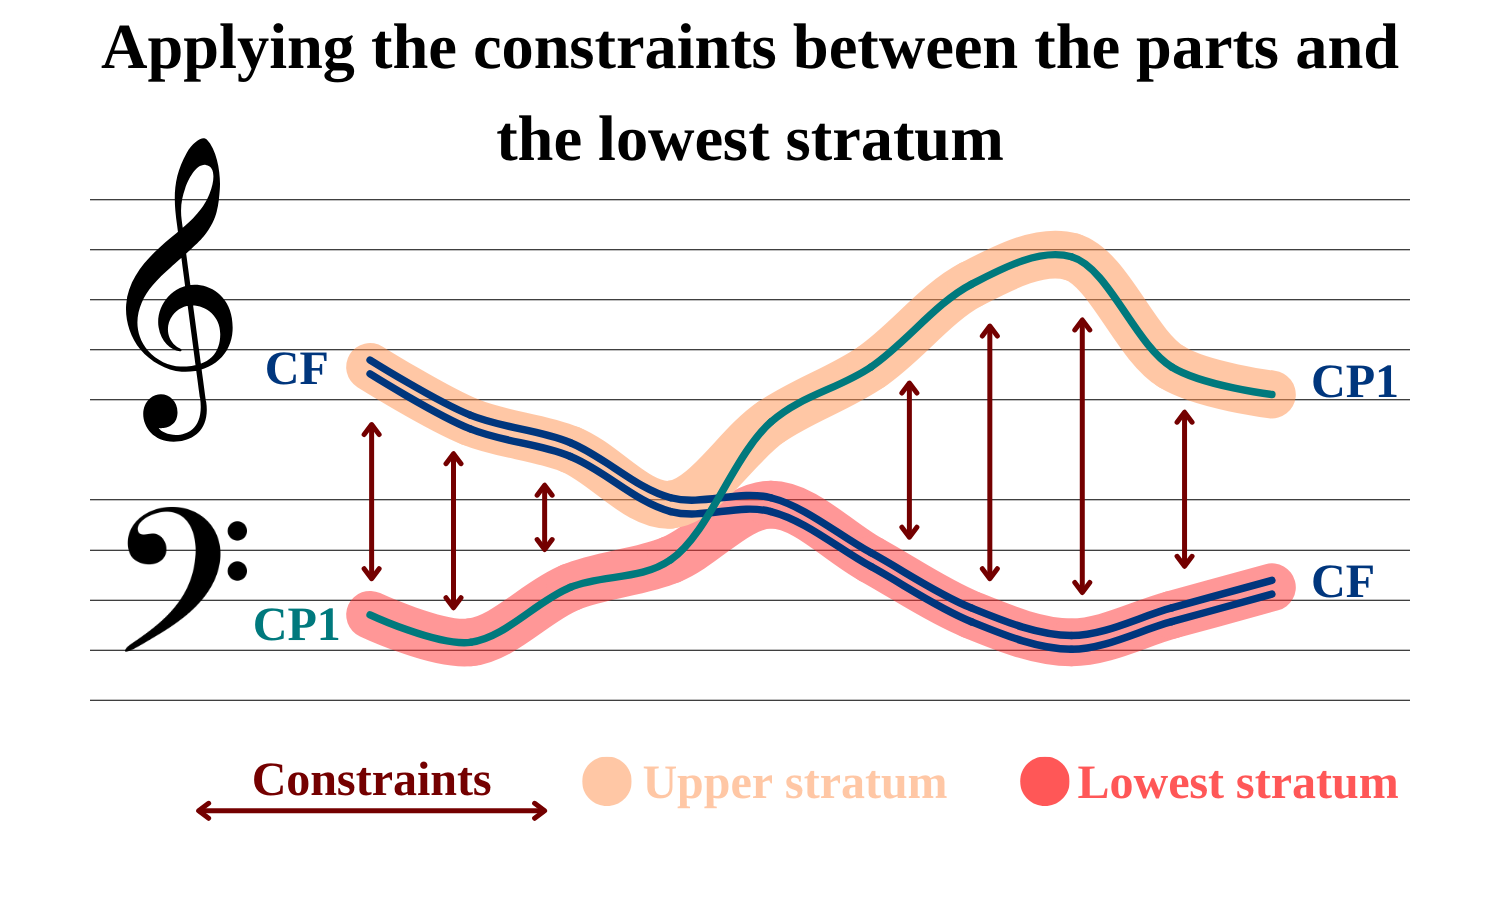
\includegraphics[width=\textwidth]{Images/p2l-2v.png}
      \captionof{figure}{Applying the constraints from the parts to the lowest stratum}
      \label{fig:p2l-2v}
\end{minipage}
\vspace{.5cm}

However, when it comes to generalising the composition of counterpoint for three voices, it is no longer possible to follow the same simplification. We are now forced to set our rules between the parts and the lowest stratum, and no longer between the counterpoints and the \cf. On figures \ref{fig:cp2cf-3v} and \ref{fig:p2l-3v}, it is made clear that establishing the rules from the counterpoints to the \cfs is really different than applying them from the various parts to the lowest stratum. In those figures, the parts don't cross and therefore match perfectly with the strata, hence the constraints are always applied to the same counterpoint. This was made for the sake of intellegibility of the graphs, but it is obviously possible that the parts cross and that the "target" of the constraints is not always the same counterpoint.

\vspace{.5cm}
\begin{minipage}{0.46\textwidth}
    \centering
    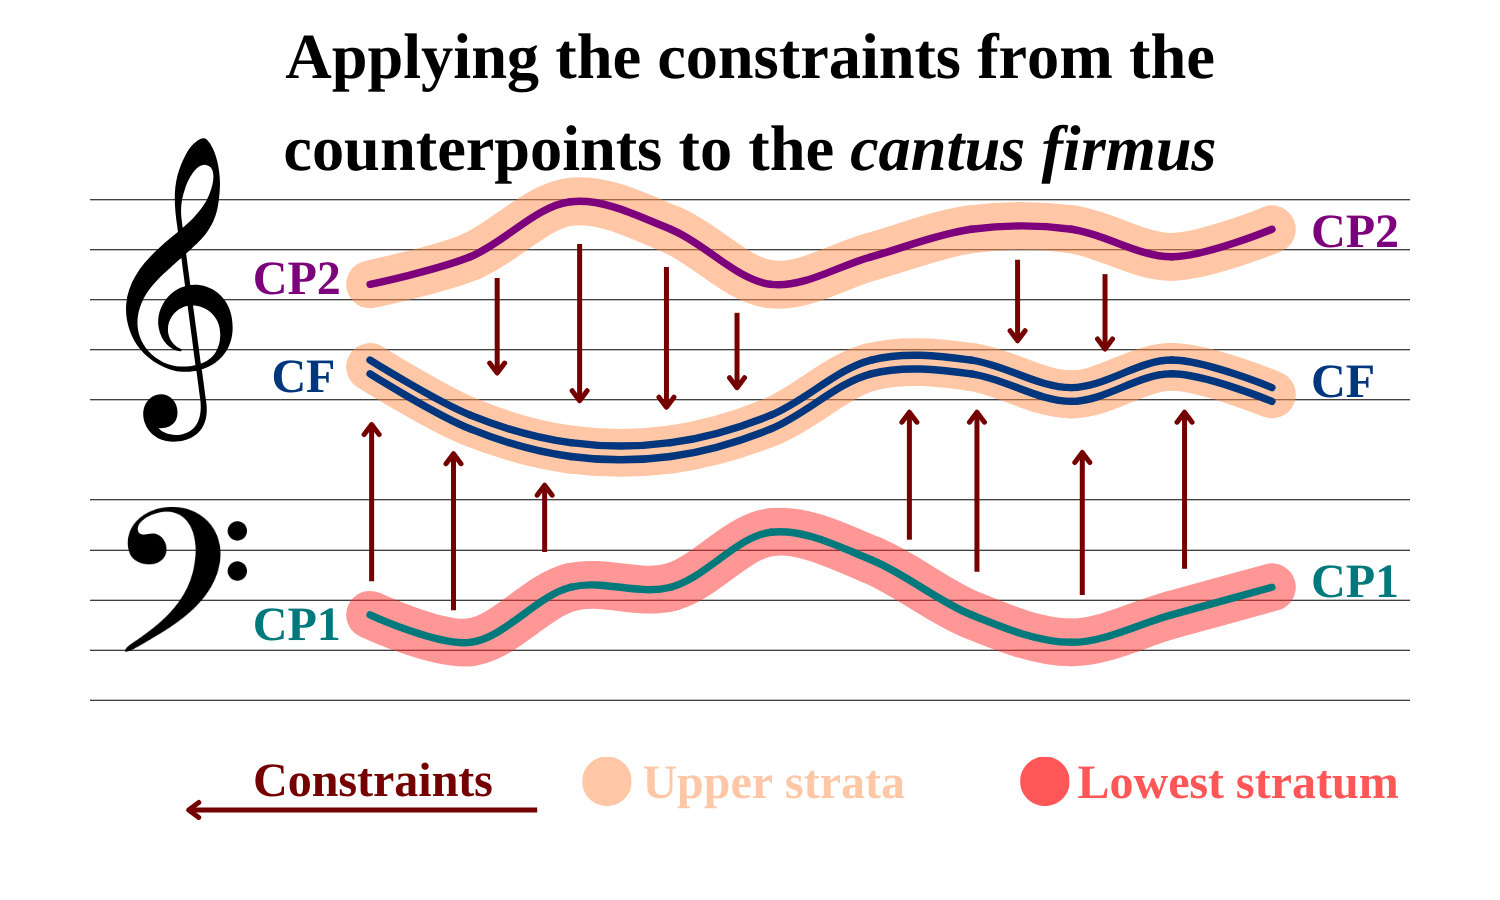
\includegraphics[width=\textwidth]{Images/cp2cf-3v.png}
    \captionof{figure}{Applying the constraints from the ctp. to the \cf}
    \label{fig:cp2cf-3v}
    \end{minipage}
    \hfill
    \begin{minipage}{0.46\textwidth}
      \centering
      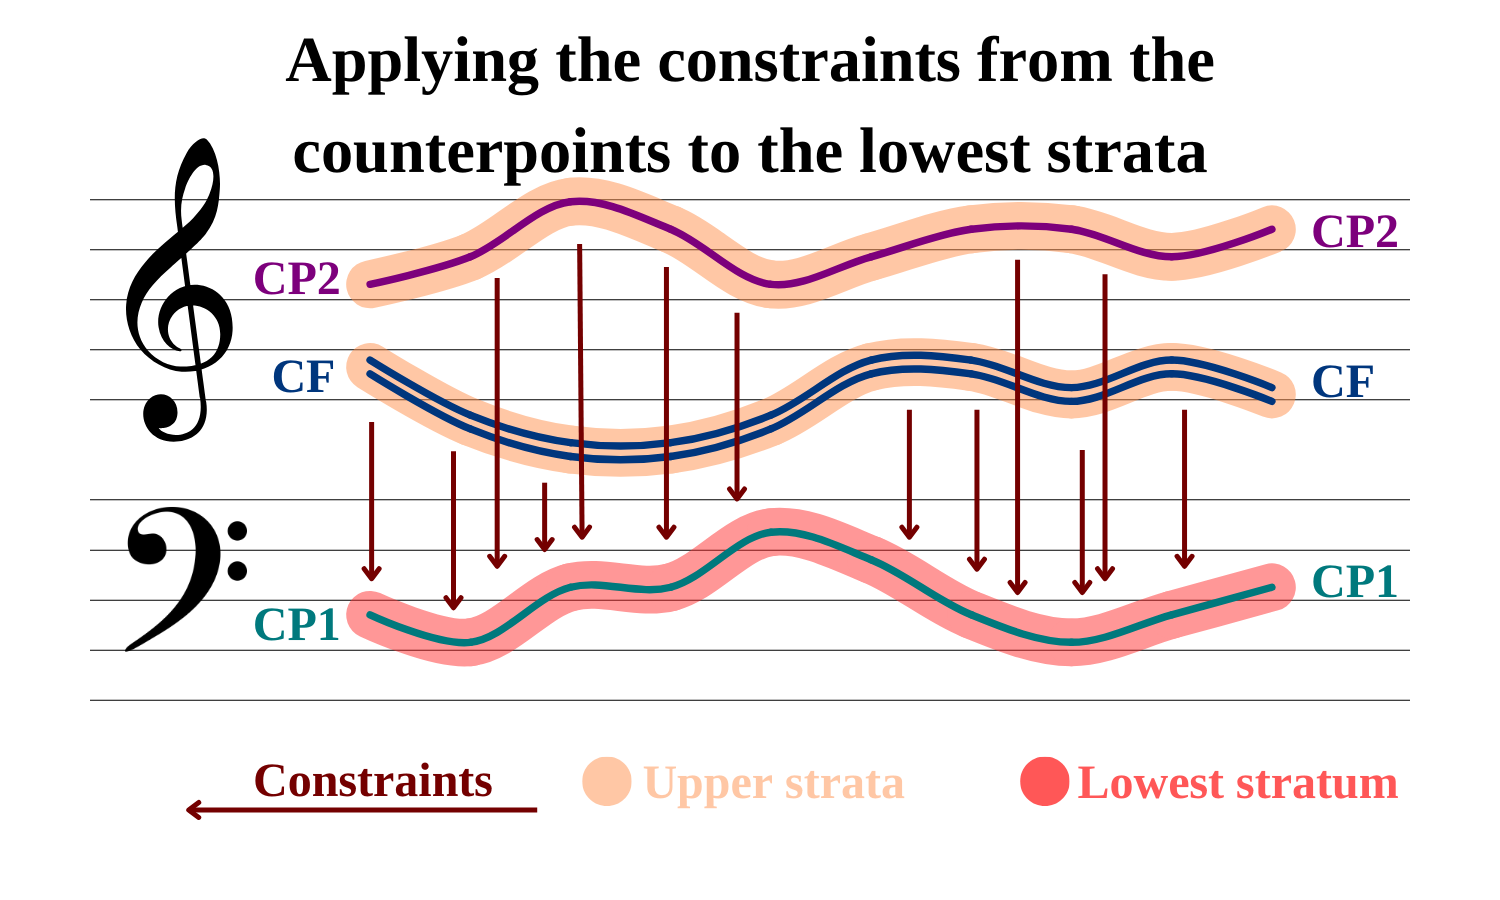
\includegraphics[width=\textwidth]{Images/p2l-3v.png}
      \captionof{figure}{Applying the constraints from the parts to the lowest stratum}
      \label{fig:p2l-3v}
\end{minipage}
\vspace{.5cm}

It is, of course, possible for the \cfs to be equal to the lowest stratum all along, in which case nothing changes from the perspective we had when composing for two voices. In this particular case, by applying the rules with respect to the \cf, we would find ourselves de facto applying the rules with respect to the lowest stratum (and we would be back to the situation described above, see figures \ref{fig:cp2cf-3v} and \ref{fig:p2l-3v}, only that there is now one more part). It is when the \cfs pitches are higher up than those of the counterpoints that considering the lowest stratum consideration becomes necessary.

\paragraph{}
A very important detail, and perhaps the biggest change brought about by this paradigm shift, is that the \cfs now becomes a counterpoint like any other, with the difference that its notes are already fixed. This means that we will treat the \cfs as a first species counterpoint (since it is always made up of whole notes), and that we will have to calculate its intervals, movements and costs, as we have already done with 'normal' counterpoints.

A second point to bear in mind, and not the least, is that all this does not mean that \textit{all} the rules are established between the parts and the lowest stratum. Certain rules will continue to apply between the different parts, regardless of whether they are high, low or intermediate.

\section{Changes induced in the variables} \label{section:changes induced}


Many changes have been induced as a result of the three part generalisation. In two part composition, it was obvious that the harmonic intervals array was describing the intervals between the \cfs and the only counterpoint, it was obvious that the motions were those of the only counterpoint, and so it goes for all the variables. When writing a three part composition, we are dealing with many possibilities when speaking about intervals or motions. Intervals between which voices? Motions of which counterpoint? To tackle this, each variable is now related to a voice.

This relationship between a variable and a voice is expressed as function. $X(v)$ represents the variable $X$ of the voice $v$. The arguments of the function can either be:
\begin{itemize}
    \item $cf$ - for linking the variable to the \cf.
    \item $cp_1$ - for linking the variable to the second \cp.
    \item $cp_2$ - for linking the variable to the third \cp.
    \item $a$ - for linking the variable to the lowest stratum.
    \item $b$ - for linking the variable to the intermediate stratum.
    \item $c$ - for linking the variable to the uppermost stratum.
  \end{itemize}

\noindent For example, $X(cf)$ refers to the variable $X$ of the \cf.

\paragraph{}
When a variable is not explicitly linked to a voice, it is implied that the relation expressed for it is true for all \textit{parts}. In other words, if the variable $X$ is written without any precision, it means $\forall v \in \{cf, cp_1, cp_2\}: X(v)$.

\paragraph{}
\noindent This change applies to all variables, namely:
\begin{itemize}
    \item \textbf{N}(v) - the notes (pitches) of voice v (this variable was written cp in T. Wafflard's thesis)
    \item \textbf{H}(v$_1$, v$_2$) - the harmonic intervals between voice v$_1$ and voice v$_2$. This variable is particular, as it needs to arguments to be meaningful.
    \item \textbf{M}(v) - the melodic intervals of voice v, 
    \item \textbf{P}(v) - the motions of voice v, 
    \item \textbf{IsCfB}(v) - the boolean array representing whether the cantus firmus is lower than a given voice,
    \item \textbf{IsCons}(v) - to the boolean array representing whether voice v is consonant or not.
\end{itemize}

\noindent It also applies to \textit{some} constants and arrays, namely:
\begin{itemize}
    \item \textbf{species}(p) - the species of part p,
    \item \textbf{n}(p) - the amount of notes in part p,
    \item \textbf{lb}(p) - the lower bound of the range of part p,
    \item \textbf{ub}(p) - the upper bound of the range of part p,
    \item $\mathcal{R}$(p) - the range of part p,
    \item \textbf{borrow}(p) - the borrowing scale of part p,
    \item $\mathcal{N}$(p) - the extended domain of part p,
    \item $\mathcal{B}$(p) - the set of beats in a measure according to the species of part p,
    \item b(p) - the number of beats in a measure according to the species of part p,
    \item d(p) - the duration of a note according to the species of part p,
\end{itemize}
Please note that the constants cannot be linked to a stratum, and only to a part. Indeed, it would have no sense to speak about the species or about the extended domain of a stratum.

The costs are also affected by the change, except for $\mathcal{C}$ (the cost factors) and $\tau$ (the total cost). The latter two remain global and are not duplicated.


To make sure that those notations are clear, here are some examples: the notation $N(a)$ corresponds to the variable representing the notes (pitches) of the lowest stratum, whereas $N(cf)$ are the notes of the \cf. The species of the second counterpoint is written $species(c)$. If only $N$ is written, then the equation in which $N$ is located holds true for any possible part (not necessary stratum). That is, the relationship $N < 60$ would mean: the pitches \textit{of all parts} must be lower than a middle C (whose representation is 60 is Open Music).

\subsection{Added constants}
Here are described some added constants, that are useful throughout the whole work.

\vspace{.5cm} \noindent \textbf{\#parts} \hspace{.2cm} \texttt{*N-PARTS}

This integer describes as many parts there are in a given problem. At this stage, it can either be equal to two (two-part composition) or to three (three-part composition). It is mainly used in the loops of the program as an end condition (\texttt{(dotimes (i *N-PARTS))})




\subsection{Added variables}
\vspace{.5cm} \noindent \textbf{A} \hspace{.cm} \texttt{is-lowest} \label{is-lowest}
% expliquer en EN que on peut pas lambda(cp1) ET lambda(cf)

A is an array of boolean variables with a size of $m$, where each variable indicates whether the corresponding part is the lowest stratum. In other words, $A(v)$ is true if v is the lowest stratum. The notation "A" was chosen as the uppercase of "a", which itself represents the lowest stratum. 
It is also worth to be noted that only one of the parts can be the lowest stratum at the time. This does not mean that two parts cannot equal the lowest stratum at the same time, it \textit{is} indeed possible that two parts blend in unison in the final chord, and that both pitches are the lowest sounding notes. It means that only one of those two is going to be considered to \textit{be} the lowest stratum (and the other one will be the intermediate stratum). This is needed in order for motions to work well. See \ref{subsubsection:one-part-per-stratum} for the details.

Here is the mathematical definition of the A array:
\begin{equation}
\begin{aligned}
\forall j \in [0, m-1)& \colon  \\
A(cf)[j] &= \,  
\begin{cases}
    \top & \text{if } N(cf)[0,j] = N(a)[0,j] \\
    \bot & \text{else }
\end{cases}\\
A(cp_1)[j] &= \,  
\begin{cases}
    \top & \text{if } (N(cp_1)[0,j] = N(a)[0,j]) \land \neg A(cf)[j] \\
    \bot & \text{else }
\end{cases}\\
A(cp_2)[j] &= \,  
\begin{cases}
    \top & \text{if } \neg A(cf) \land \neg A(cp_1)\\
    \bot & \text{else }
\end{cases}
\end{aligned}
\end{equation}

As can be seen in these equations, only the downbeat of each measure is taken into account when computing the A array. The reason for this is that it is the downbeat note that determines which chord will be \textit{the} chord of the measure, and the other beats are just fioritures. Another reason for this is also that it is only going to serve in contexts where the first note of the measure is relevant.

\paragraph{}
In practice, there is only an \texttt{is-not-bass} array in the code (which is then equal to $\neg A$), as it is almost always more useful to know if a part is \textit{not} the lowest stratum than knowing if it is the lowest one. 

\subsection{Modified constants} \label{subsection:modified_constants}
\noindent \textbf{species} \hspace{.2cm} \texttt{species} 

The species constant, which represents the species of a given part, can now take a value between zero and five (inclusive). The value zero is specific to the \cfs (which can be understood as a simplified first species counterpoint). This constant is more useful in the code than in the mathematical notations.
\begin{equation}
species(v) = 0 \iff v = cf
\end{equation}

\subsection{Modified variables} \label{subsection:modified_variables}
Given that the majority of the rules now apply between parts and the lowest stratum, the meaning of the variables has been modified to adapt to this reality. 

\vspace{.5cm} \noindent \textbf{N}(v) \hspace{.2cm} \texttt{notes} 

We changed the name of former \texttt{cp} array and renamed it to \texttt{N} (for notes), for the sake of clarity. As we have now three of those arrays (one for the first counterpoint, one for the second counterpoint, and even one for the \cf), it needed a less ambiguous name than the one it had before.
It still works exactly the same. It is an array of size $s_m$ representing the pitches of a given voice at a given beat in a measure.



\vspace{.5cm} \noindent \textbf{H}$_{(\text{abs})}$(v$_1$, v$_2$) \hspace{.2cm} \texttt{h-intervals}\hspace{.2cm} \texttt{h-intervals-abs}\hspace{.2cm} \texttt{h-intervals-to-cf}\hspace{.2cm}  ...
%todo must be reworked

The way in which this variable works remains much the same, i.e. it represents the interval between one voice and another. This definition has been extended to include intervals other than that between the counterpoint and the \cf. Thus, $H(v1,v2)[i,j]$ represents the intervals between the $i$th beat of voice $v_1$ and the \textit{first} beat of voice $v_2$. $v_1$ may be a part and $v_2$ may be a stratum, as you can calculate harmonic intervals between a part and a stratum. When no $v_2$ is precised, it is equal to $a$, by default. In other words, $H(v_1)$ represents the intervals between the voice $v_1$ and the lowest stratum: $H(v_1) := H(v_1,a)$.

Here is the generalisation explained above, matching to the current definition of the harmonic intervals array:
\begin{equation}
\begin{aligned}
    &\forall v_1, v_2 \in \{cf, cp_1, cp_2\}, \quad \forall i \in \mathcal{B}(v_1), \quad \forall j \in [0, m):\\
    &H_{abs}(v_1,v_2)[i, j] = \left|N(v_1)[i, j] - N(v_2)[0,j]\right|\\
    &H(v_1-v_2)[i, j] = H_{abs}[i, j]\ \text{mod}\ 12\\
    &\text{where } H_{abs}[i, j] \in [0, 127], H[i, j] \in [0, 11]
\end{aligned}
\end{equation}

\vspace{.5cm}
\noindent \textbf{M}$_{\text{brut}}$(s) \hspace*{.2cm} \texttt{m-intervals-brut}

The variable M(p) (i.e. when related to a part) keeps representing the melodic intervals of the voice v and its way of working remains intact. What is described here is its working when related to a stratum, and more specifically, to the lowest stratum. Since strata don't have melodic intervals \textit{per se} (they actually do have melodic intervals, but it doesn't really make sense to consider them), we need to redefine what we mean when speaking about their melodic intervals. Thus, the melodic intervals of the lowest stratum are defined like this: the melodic interval in measure $j$ of the lowest stratum is equal to the last melodic interval in measure $j$ of the part that is the lowest stratum in measure $j+1$. This complex definition is needed in order for the computation of the motions to work fine. The motions of the lowest stratum are an abstract notion that serves only in formulas and constraints and \textit{does not intend to represent any concrete motion really happening in the composition, nor does it correspond to the melodic intervals between the pitches of the lowest stratum}.

\begin{equation}
    \begin{aligned}
        &\forall j \in [0, m-2):\\
        &M_{brut}(a)[j] = \,  
        \begin{cases}
            M_{brut}(cf)[0][j] & \text{if } A(cf)[j+1]\\
            M_{brut}(cp_1)[\text{max}(\mathcal{B}(cp_1))][j] & \text{if } A(cp_1)[j+1]\\
            M_{brut}(cp_2)[\text{max}(\mathcal{B}(cp_1))][j] & \text{if } A(cp_2)[j+1]\\
        \end{cases}
    \end{aligned}
\end{equation}

\noindent It might be helpful to have a look at figures \ref{fig:stratum-m-intervals-1} and \ref{fig:stratum-m-intervals-2} to understand better how the melodic intervals arrays for the lowest stratum.

\vspace{.5cm}
\begin{minipage}{0.46\textwidth}
    \centering
    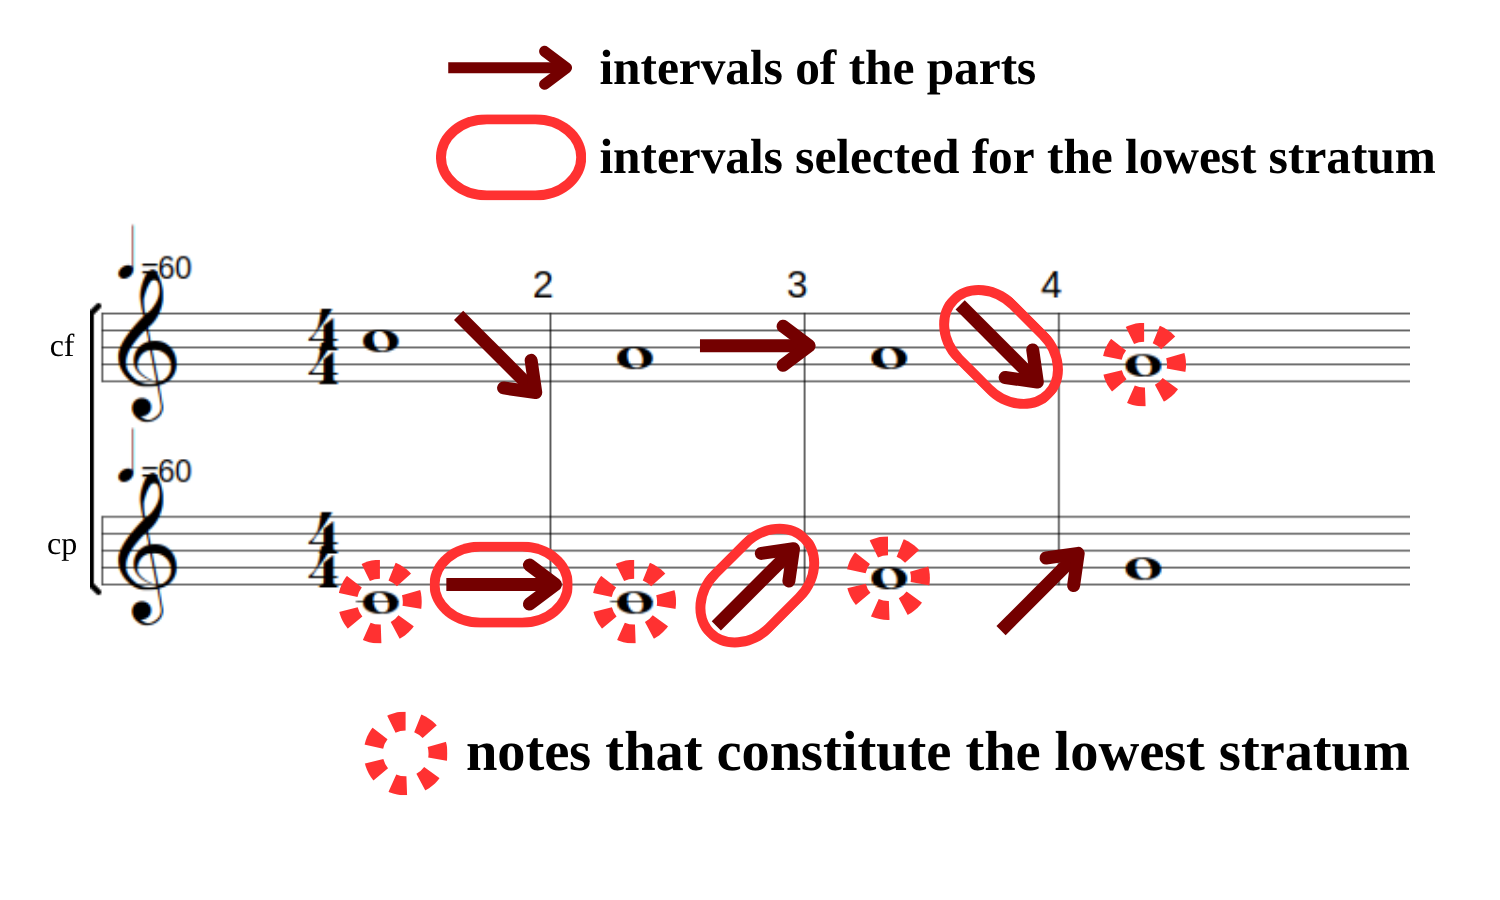
\includegraphics[width=\textwidth]{Images/stratum-m-intervals.png}
    \captionof{figure}{Understanding the melodic intervals of the lowest stratum with a first species counterpoint}
    \label{fig:stratum-m-intervals-1}
    \end{minipage}
    \hfill
    \begin{minipage}{0.46\textwidth}
      \centering
      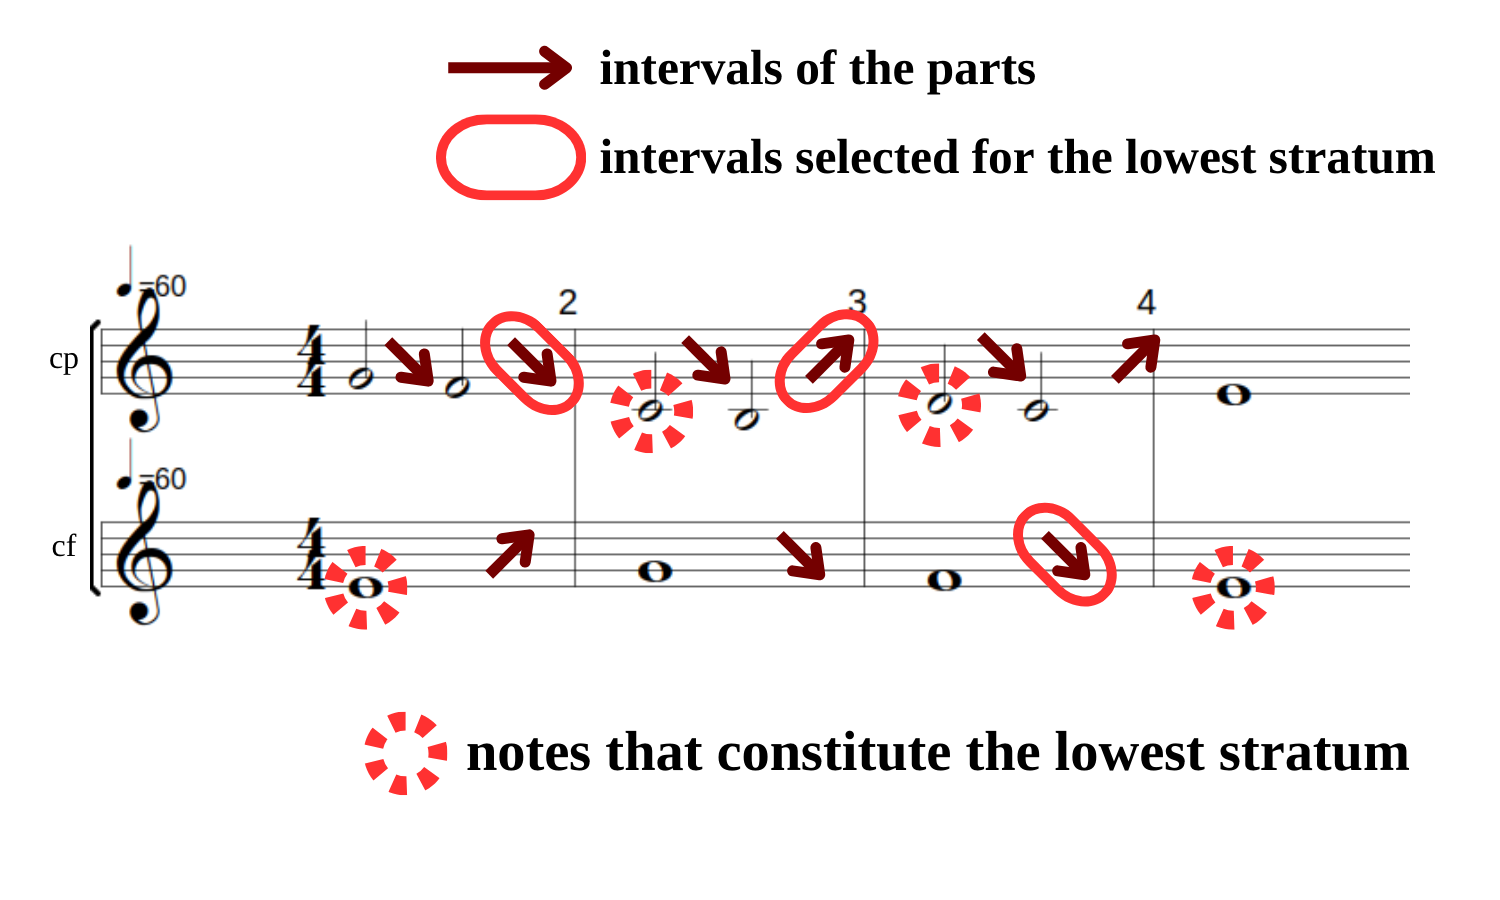
\includegraphics[width=\textwidth]{Images/stratum-m-intervals2.png}
      \captionof{figure}{Understanding the melodic intervals of the lowest stratum with a second species counterpoint}
      \label{fig:stratum-m-intervals-2}
\end{minipage}
\vspace{.5cm}

\section{Exploring the interaction of the parts with the lowest stratum}



\vspace{.5cm}
\noindent \textbf{P}(v) \hspace*{.2cm} \texttt{motions}

The motions array was redefined to compute the motions of a voice v with respect to the lowest stratum, instead of computing them with respect to the \cf. 

Motions are now calculated according to the movements of the lowest stratum. This might be counterintuitive because strata have no  The problem here is that if a part is also the lowest stratum, we end up calculating the motion between a part and itself. This inevitably leads to direct motions being calculated, because a part is always moving in the same direction as itself. To solve this problem, the motions of a part are now equal to -1 when the part is also the lowest stratum (denoted A, see section \ref{is-lowest}). 
\begin{equation}
\begin{aligned}
&\forall v \in \{cf, cp_1, cp_2\}, \quad \forall x \in \{1, 2\}, \quad \forall i \in B, \quad \forall j \in [0, m - 1),\quad x := b - i\\
    motions(v)[i,j]& = \,  
    \begin{cases}
        0 & \land (M_{brut}^{x}(v)[i, j] > 0 > M(a)_{brut}[j]) \vee\, (M_{brut}^{x}(v)[i, j] < 0 < M(a)_{brut}[j]) \\
        1 & M_{brut}^{x}(v)[i, j] = 0  \oplus M(a)_{brut}[j]=0 \\
        2 & (M_{brut}^{x}(v)[i, j] > 0 \land M(a)_{brut}[j] > 0) \vee\, (M_{brut}^{x}(v)[i, j] < 0 \land M(a)_{brut}[j] <0)
    \end{cases} 
    \\
    P(v)[i,j]& = \,  
    \begin{cases}
        -1 & \text{if } A(v)[j] \\
        motions(v)[i,j] & \text{if } \neg A(v)[j]
    \end{cases}
\end{aligned}
\end{equation}

\chapter{Formal rules for three-part counterpoint}\label{chapter:species}
The purpose of this section is to extract all the rules that Fux mentions in his work and to make sure that they are unambiguous.

It consists of seven subsections: first, a section for the implicit rules (the rules that Fux doesn't mention, but are present in all his examples), then a section for each species, and finally a short section that considers the interaction between different species. There is no section on rules for all species, yet there \textit{are} rules that apply to all species. In fact, all the rules mentioned in the first species section also apply to the other species. Although Fux doesn't explicitly mention this point, it becomes clear when you look at how he teaches and applies these rules in composition.Therefore, the rules for all species are in the first species section. The reason these rules are in the first type section is because Fux himself mentions these rules in his chapter on first type counterpoint.

Each species subsection is divided into two parts: the first part is about setting up Fux's rules and discussing them. The second part is about translating the rules into formal logic.

\paragraph*{Some important notes}
\begin{itemize}
    \item \textbf{Concerning the green dot} ---
    Please note that all the rules from T. Wafflard's thesis still apply to three-part compositions. The numbering of the rules in this work is the same as in T. Wafflard's work. If a rule is defined with the same number as an existing rule for two-part compositions, this means that the corresponding rule from T. Wafflard's work does not apply to three-part compositions, and that the new rule should be used instead. To make this clearer, there is a green dot (\greendot) next to the rules from T. Wafflard's thesis that got redefined when used in a three-voice composition.
    \item \textbf{Concerning the \texttt{[PREF]} marker} ---
    As discussed earlier (see Section~\ref{subsection:preferences-vs-hard-rules}), some rules are mandatory and must be followed to find a valid solution, and other rules are just preferences that can be followed to find a \textit{better} solution. The preferences have been marked '\texttt{[PREF]}' throughout the chapter to make it clearer which rule is mandatory and which is a preference.

    \item \textbf{Concerning the default costs} --- Each time a cost is mentioned in the formalisation rules, the value corresponding to it is its default value, as defined in Appendix~\ref{chapter:user-guide}. Note, however, that in practice the value for each cost can be changed by the user to suit their needs.
    \item \textbf{Concerning the purpose of all the rules} --- 
    It may be interesting to remember the purpose of these rules. Some rules are concerned with musicality: composing counterpoint that sounds nice; for example, the rule that forbids dissonance. Some rules are concerned with singability: composing counterpoint that is not too difficult for the human voice to sing; for example, the rule forbidding a melodic leap greater than a sixth.

\end{itemize}

\section{Implicit rules}
These implicit rules apply to all types of counterpoint. They are never explicitly defined by Fux, but are derived from his many examples. These implicit rules are therefore actually used by Fux, even though he doesn't talk about them.

\subsection{Formalisation in English} \label{sec:generalenglish}
\begin{enumerate}[wide, label=\bfseries 1.H2 and 1.H\arabic*]
    \setcounter{enumi}{2} % Start from 8
    \item \greendots \textit{First and last notes have not to be perfect consonances anymore.} \label{rule:last-chord-not-perfect-anymore}    

    Fux doesn't state this in his text, but in many of his examples, we see that when he composes with three voices (and more), the first and last harmonic intervals between the parts and the lowest stratum are not necessary a perfect consonance anymore.
\end{enumerate}

\begin{enumerate}[wide, label=\bfseries 1.H7 and 1.H\arabic*]
    \setcounter{enumi}{7} % Start from 8
    \item \greendots \textit{The harmonic interval of the penultimate measure must be either a minor
    third, a perfect fifth, a major sixth, or an octave.} \label{rule:penult-interval-3-voices}
    
    In two-part composition rules, Fux said that the last harmonic interval had to be either a minor or a majord third (see rule~\ref{rule:penult-interval-2v} for two voices). This is something he doesn't respect at all in three-part composition, but we can see that he still tries to use minor third and major sixths when possible, in the penultimate measure. The rule from two-part species was thus rewritten in order to be appropriate: either use a perfect consonance, a minor third, or a major sixth.
\end{enumerate}

\begin{enumerate}[wide, label=\bfseries G\arabic*]
    \setcounter{enumi}{7} % Start from 8

    \item\label{rule:last-chord-h-triad} \textit{The last chord must be composed only of the notes of the harmonic triad.} 

    Again, this isn't stated explicitly, but we see that all of his examples end with a chord containing exclusively the notes of the harmonic triad.
    
    \item \textit{The last chord must have the same fundamental as the one of the scale used throughout the composition.}\label{rule:same-fundamental}

    This rule emanates from an observation of Fux's examples throughout the chapter. The last chord of all his compositions always have the same fundamental as the fundamental of the scale used throughout the composition.
    When the \textit{cantus firmus} is the lowest stratum, this is not a problem, as the \textit{cantus firmi} always end with the fundamental note of the scale. But when not, it has to be imposed by a constraint, or we may end up with surprising results.
\end{enumerate}

\subsection{Formalisation into constraints} \label{sec:generalconstraints}
    \paragraph{\hspace{0.6cm}\ref{rule:last-chord-not-perfect-anymore}} \greendots \textit{First and last notes have not to be perfect consonances anymore.}

    There is no constraint associated with this rule, as it is a relaxation of a rule from the two-part composition rule set.

    \paragraph{\hspace{0.6cm}\ref{rule:penult-interval-3-voices}} \greendots \textit{The harmonic interval of the penultimate measure must be either a minor third, a perfect fifth, a major sixth, or an octave.}
    \begin{equation}
        \begin{aligned}
            H[0, m-2] \in \{0, 3, 7, 9\}
        \end{aligned}
    \end{equation}

    \paragraph{\hspace{0.6cm}\ref{rule:last-chord-h-triad}} \textit{The last chord must be composed only of the notes of the harmonic triad.} 
    
    \begin{equation} \begin{aligned}
    \forall s \in \{b, c\} \colon H(s)[0, m-1] \in Cons_{h\_triad}
    \end{aligned} \end{equation}

    \paragraph{\hspace{0.6cm}\ref{rule:same-fundamental}} \textit{The last chord must have the same fundamental as the one of the scale used throughout the composition.}\label{constraint:same-fundamental}

    Since the fundamental of the scale is defined by being the first note of the \textit{cantus firmus}, we impose that the last note of the lowest stratum must be equal to the first one of the \textit{cantus firmus} (taking the modulos into account).
    
    
    \begin{equation} \begin{aligned}
    N(a)[0, m-1] \mod 12 = N(\mathit{cf})[0, 0] \mod 12
    \end{aligned} \end{equation}

\section{First species}
This section deals with the rules that apply to the first species of counterpoint. As mentioned earlier, these rules apply to \textit{all} species in the context of a three-part composition. In other words, these rules apply whenever $species(p) \in \{0, 1, 2, 3, 4, 5\}$. More specifically, the rules in this section apply to the first beat of each species, except for the fourth species, where they apply to the third beat (see the note on the fourth species~\ref{nota-bene-4th-species}).

\paragraph{}
The first species consists of whole notes only. It is the basis of counterpoint and its simplest case. 

\begin{figure}[h]
    \centering
    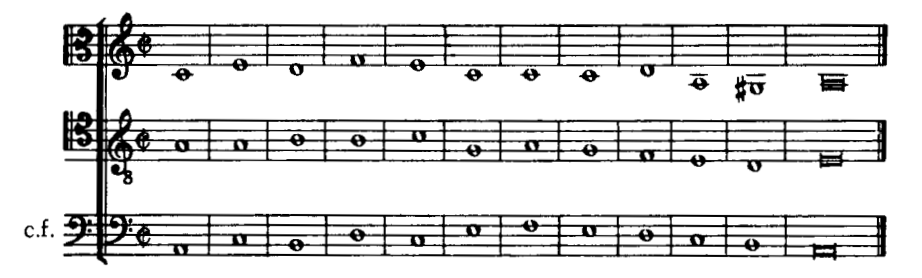
\includegraphics[width=1\textwidth]{Images/Species_examples/1sp-example.png}
    \caption{Example of a first species counterpoint in three-part composition}
    \label{fig:example-1sp}
\end{figure}

\subsection{Formalisation into English}
\subsubsection{Structural constraints}
\begin{enumerate}[wide, label=\bfseries 1.S\arabic*]
    \item\label{rule:allwhole} \textit{All notes are whole notes.}
     
    \begin{quotation}
       "This species consists of three whole notes in each instance."
       \textcite[p.71]{GaPEng}
   \end{quotation}

   This pretty straightforward rule is the very definition of the first species. It adds nothing in comparison with the rules for the two part comparison. It is hence already implemented by the first species for two voices and does not need any consideration. 
\end{enumerate}
\subsubsection{Harmonic rules}
\begin{enumerate}[wide, label=\bfseries 1.H\arabic*]
    \item\label{rule:consonant} \greendots \textit{All notes on the downbeat are consonant with the notes of the lowest stratum.}
     
    \begin{quotation}
       "This species consists of three notes, the upper two being consonant with the lowest."
       \textcite[p.71]{GaPEng}
   \end{quotation}

   This rule is an update of previous \textbf{1.H1} (that previously was saying that \textit{all} intervals must be consonants). Fux states that the upper voices and the lowest one are consonant, and not all voices together. 
    
    \setcounter{enumi}{7} % Start from 8

    \item\label{rule:harmonic-triad} \texttt{[PREF]}  \textit{The harmonic triad should be used as much as possible.} 

    \begin{quotation}
    "The harmonic triad should be employed in every measure if there is no special reason against it."
    \textcite[p.71]{GaPEng}
    \end{quotation}

    As a footnote states it \cite[footnote, p.71]{GaPEng}, Fux refers to the "harmonic triad" as being a chord in this position: 1-3-5 (contrary to what is today understood as a harmonic triad).
    The rule says it is not obligated, but it is preferred, to use the 1-3-5 chord, considering that 1 is the lowest voice.
    

    \item\label{rule:sixth-or-octaves}  \textit{One might use sixths or octaves.}

    \begin{quotation}
    "Occasionally, one uses a consonance not properly belonging to the triad, namely, a sixth or an octave."
    \textcite[p.72]{GaPEng}
    \end{quotation}

    Here, Fux explains that when it is not possible to have a harmonic triad, you can use sixths or octaves instead. Remember that the sixths or the octaves are calculated from the lowest stratum. Since the rule~\ref{rule:consonant} obligates the use of a perfect consonance (i.e. a third, a fifth, a sixth or an octave), when the harmonic triad cannot be used, it is already naturally replaced by a third or a sixth, because no other intervals are allowed. It is thus not a new rule but a restatement of rule~\ref{rule:consonant}.    

    \item\label{rule:tenth-is-last-chord}  \textit{Tenths are prohibited in the last chord.}

    \begin{quotation}
    "One feels that the degree of perfection and repose which is required of the final chord does not become sufficiently positive with this imperfect consonance [(speaking about a tenth)]."
    \textcite[p.77]{GaPEng}
    \end{quotation}

    When Fux says this, he takes a tenth as an example, but it here understood that the final chord cannot include a tenth (third + octave), nor an eight-teenth (third + two octaves), etc. Nevertheless, "simple" third are considered completely valid.

    \item\label{rule:unison-vs-octave} \texttt{[PREF]} \textit{Octaves should be preferred over unisons.}

    \begin{quotation}
    "Unison is less harmonious than the octave."
    \textcite[p.79]{GaPEng}
    \end{quotation}

    This rule does not bring anything new, as there is already a rule stating that two parts cannot blend in unison (\ref{rule:no-unison-appendix}). If no unison is possible, then the octaves will always be preferred over the unison (since the latter is not possible).

    \item\label{rule:minor-third}  \textit{Last chord cannot include a minor third.}

    \begin{quotation}
    "The minor third is not capable of giving a sense of conclusion."
    \textcite[p.80]{GaPEng}
    \end{quotation}

    Fux later states that minor modes should not include a third altogether, but that sometimes it is impossible to do without it, so the major third \textit{is} allowed in minor modes.

\end{enumerate}

\subsubsection{Melodic rules}
The following rules obviously don't apply to the \cf, since its melody is already fixed.
\begin{enumerate}[wide, label=\bfseries 1.M\arabic*]
\setcounter{enumi}{2} % Start from 3
    \item\label{rule:steps-prefered} \texttt{[PREF]} \textit{Steps are preferred to skips.}

    \begin{quotation}
    "[Each part] follows the natural order closely."
    \textcite[p.73]{GaPEng}
    \end{quotation}

    After having said this, Fux complements his explication by saying the counterpoints should be "moving gracefully, stepwise without any skip". This is clearly a preference, and has already been covered when implementing the first species for two voices (see~\ref{rule:smallmelody}). It can thus be ignored in the scope of this thesis.

    \item\label{rule:variety} \texttt{[PREF]}  \textit{The notes of each part should be as diverse as possible.}

    \begin{quotation}
    "[Each part] follows the principle of variety."
    \textcite[p.73]{GaPEng}
    \end{quotation}

    Fux never clearly defines what he means by the "principle of variety". So we try to define it according to what we can read in his work. The examples he gives are a great help. He first writes an incorrect example and then corrects it, saying that the corrected example is better because it follows the principle of variety more closely. The difference between the two examples is that the number of different pitches has been increased. So we can define the principle of variety as: use as many different notes as possible in a single voice. 

    The principle of variety is therefore clearly a preference.

    This principle is very interesting because it introduces the only rule \textit{across all} rules that has a scope greater than two measures. While without this rule the solver uses constraints that apply only to one measure (think of harmonic constraints) or sometimes to two measures (think of melodic constraints), this constraint is the first to give the solver some "memory" about the composition. And although seven measures may seem like a small range, it means that the constraint covers a large part of the composition (when dealing with compositions of 10 to 15 measures, of course).

    \item\label{rule:each-part-should-stay-in-its-voice-range}  \textit{Each part should stay in its voice range.}

    \begin{quotation}
    "One should not exceed the limits of the five lines without grave necessity."
    \textcite[p.79]{GaPEng}
    \end{quotation}

    Fux says here that each part should stay on the musical staff (Fux's "five lines"). Since every staff can be represented differently according to the clef that is used, this rule could be always true. Obviously, Fux meant the staff corresponding to the voice range (treble clef for a soprano, bass clef for a bass, ...). 
    
    This is actually something that is already handled when declaring the $N(p)$ arrays, as they are declared with an upper and lower bound ($ub(p)$ and $lb(p)$), corresponding to their voice range.

    \item\label{rule:melodic-intervals-cannot-be-greater-or-equal-to-a-sixth}  \textit{Melodic intervals cannot be greater or equal to a sixth.}

    \begin{quotation}
    "The skip of a major sixth is prohibited."
    \textcite[p.79]{GaPEng}
    \end{quotation}
    
    This rule is only a restatement of rule~\ref{rule:mlesixth}, saying that melodic intervals cannot exceed a minor sixth interval.
\end{enumerate}

\subsubsection{Motion rules}
\begin{enumerate}[wide, label=\bfseries 1.P\arabic*]
    \item\label{rule:direct-to-p-cons} \greendots \texttt{[PREF]}  \textit{Reaching a perfect consonance by direct motion should be avoided.}

    \begin{quotation}
    "[Reaching] perfect consonance by direct motion [is allowed if] there is no other possibility."
    \textcite[p.77]{GaPEng}
    \end{quotation}

    This is a new rule as it only applies to three-part composition, but it cancels an already existing rule that used to be applied in two-part composition. The same rule in two-part composition states that it is prohibited to reach a perfect consonance using a direct motion. In three-part composition, this is not prohibited anymore, as not doing it is sometimes impossible, and you may thus derogate from this rule.

\setcounter{enumi}{3} % Start from 4
    \item\label{rule:succ-p-cons} \texttt{[PREF]} \textit{Successive perfect consonances should be avoided.}

    \begin{quotation}
    "The necessity of avoiding the succession of two perfect consonances [...]."
    \textcite[p.72]{GaPEng}
    \end{quotation}

    Fux implies here that there should not be two consecutive perfect consonances. He does not specify whether this rule applies to all three parts at once (i.e. if there was a consonance between part 1 and part 2 in measure X, there cannot be one between part 2 and 3 in measure X+1), or whether it applies to each pair of parts separately. However, in his example (Fig. 91 of the English version \cite{GaPEng}) we can clearly see that there is a perfect consonance in every measure (parts 1-3, then 1-2, then 1-3, then 2-3, then 1-2). From this we can deduce that \textit{for each pair of parts} it is forbidden for two perfect consonances to follow each other.

    However, a closer look at his examples throughout the book reveals that Fux does not respect this rule at all. To name just a few places where this rule does not apply, let's mention figure 108, in the first three measures, between the bass and the \cf; figure 109, in the same place, between the \cfs and the alto; figure 110, in measures 8 and 9, between the bass and the alto. For this reason, this rule must be considered as a preference rather than an absolute constraint.

    To make this a preference is still very surprising, since many authors of counterpoint consider the succession of perfect consonances to be completely forbidden \cite{Bitsch}. However, we are concentrating here on the Fux formalisation, and the possibility of completely forbidding perfect consonance successions is a choice offered to the user in the interface.

    \item\label{rule:start-distant}  \textit{Each part starts distant from the lowest stratum.}

    \begin{quotation}
    "To allow enough space for the voices to move toward each other by contrary motion, the upper voices begin distant from the bass."
    \textcite[p.75]{GaPEng}
    \end{quotation}

    This preference cannot be made clearer: the voices start distant from the lowest stratum.

    \item\label{rule:same-movement}  \textit{It is prohibited that all parts move in the same direction.}

    \begin{quotation}
    "All voices ascend[ing] [is] a progression which can hardly be managed without awkwardness resulting."
    \textcite[p.76]{GaPEng}
    \end{quotation}

    What Fux is explaining here is simply that the three parts cannot move in the same direction. In other words, if two voices go up, the last one cannot go up. If two voices go down, the last one cannot go down. And if two voices stand still, the last one must move.

    \item\label{rule:ascending-sixths}  \textit{It is prohibited to use successive ascending sixths on a direct upwards motion.}

    \begin{quotation}
    "Ascending sixths on the downbeat sound harsh."
    \textcite[p.77]{GaPEng}
    \end{quotation}

    This rule is quite simple and states that if one harmonic interval is a sixth, then the next harmonic interval cannot also be a sixth.
\end{enumerate}

\subsection{Formalisation into constraints}
\subsubsection{Structural constraints}
    \paragraph{\hspace{0.6cm}\ref{rule:allwhole}} \textit{All notes are whole notes.}
    
    This rule needs no special constraint, since it is the very definition of the first species to consist only of whole notes.

\subsubsection{Harmonic rules}
\paragraph{\hspace{.6cm}\ref{rule:consonant}} \greendots \textit{All notes on the downbeat are consonant with the notes of the lowest stratum.}
    
    The new definition of variable H already captures the change in the rule. This means that the equation of rule~\ref{rule:allcons} stays the same.
    \paragraph{\hspace{.6cm}\ref{rule:harmonic-triad}} \texttt{[PREF]} \textit{The harmonic triad should be used as much as possible.}
    
    As this rule is actually a preference and not a mandatory rule, it has been implemented as a cost. If the harmonic triad is used, then the cost is 0. Else, it is 1.
    % todo should not be 1 absolutely, should depend on the user
    \begin{equation}
    \begin{aligned}
    &\forall j \in [0, m-1) \colon \\
    &(H(b)[0,j] \notin \{3, 4\}) \lor (H(c)[0, j]  \neq 7) \iff \mathcal{C}_{\mathit{prefer-harmonic-triad}}[j] = 1
    \end{aligned}
    \end{equation}

    \paragraph{\hspace{.6cm}\ref{rule:sixth-or-octaves}}  \textit{One might use sixths or octaves.}

    As discussed in~\ref{rule:sixth-or-octaves}, there is no constraint to add for this rule.
    
    \paragraph{\hspace{.6cm}\ref{rule:tenth-is-last-chord}}  \textit{Tenths are prohibited in the last chord.}

    \begin{equation} \begin{aligned}
    &H_{brut}[0, m-1] > 12 \implies H[0, m-1] \notin \{3, 4\}
    \end{aligned} \end{equation}

    If the harmonic interval is bigger than an octave, then you cannot use thirds anymore.

    \paragraph{\hspace{.6cm}\ref{rule:unison-vs-octave}} \texttt{[PREF]} \textit{Octaves should be preferred over unisons.}

    As discussed before, there is no constraint to add for this rule.

    \paragraph{\hspace{.6cm}\ref{rule:minor-third}}  \textit{Last chord cannot include a minor third.}

    \begin{equation} \begin{aligned}
    H[0, m-1] \neq 3
    \end{aligned} \end{equation}

\subsubsection{Melodic rules}
\paragraph{\hspace{.6cm}\ref{rule:steps-prefered}} \texttt{[PREF]} \textit{Steps are preferred to skips.}

As discussed in~\ref{rule:steps-prefered}, there is no constraint to add as it already exists (see~\ref{rule:smallmelody}).

\paragraph{\hspace{.6cm}\ref{rule:variety}} \texttt{[PREF]}  \textit{The notes of each part should be as diverse as possible.}

    As it is not explained either if this has to be true for the whole partition or only for two following notes, it has been chosen as an arbitrary seven successive notes to apply the rule on. This means that the solution is penalized if a note in measure X was already present in measures [X-3, X+3]. This amount was chosen because it represents the number of flat notes that exist, pushing for the solver to find a solution that contain all of them.

    \begin{equation} \begin{aligned}
    &\forall p \in \{cp_1, cp_2\}, \quad \forall j \in [0, m), \quad \forall k \in [j+1, \text{min} (j+3, m-1)] :\\ 
    &N(p)[0, j] = N(p)[0, j+k]\iff \mathcal{C}_{variety}[j+m*k]= 2
    \end{aligned} \end{equation}

    \paragraph{\hspace{.6cm}\ref{rule:each-part-should-stay-in-its-voice-range}}  \textit{Each part should stay in its voice range.}

    As was discussed before, there is no constraint associated to this rule, as it is already covered by the definition of the voice range.

    \paragraph{\hspace{0.6cm}~\ref{rule:melodic-intervals-cannot-be-greater-or-equal-to-a-sixth}}  \textit{Melodic intervals cannot be greater or equal to a sixth.}

    As was said before, no constraint must be implemented for this rule as it is a restatement of rule~\ref{rule:mlesixth}.

\subsubsection{Motion rules}
\paragraph{\hspace{.6cm}\ref{rule:direct-to-p-cons}} \greendots \texttt{[PREF]} \textit{Reaching a perfect consonance by direct motion should be avoided.}

    Since there is no way in constraint programming to implement a rule that must be obeyed only if possible other than by using a cost, the initial constraint was rewritten to a new one.

    \begin{equation} \begin{aligned}
    &\forall j \in [0, m-1) :\\
    &P[0, j] = 2 \land H[0, j+1] \in Cons_{p} \iff \mathcal{C}_{\text{{direct\_move\_to\_p\_cons}}}[j] = 8
    \end{aligned} \end{equation}

    Remember: $P[0,j] = 2$ means that the motion is direct.
    
\paragraph{\hspace{.6cm}\ref{rule:succ-p-cons}} \texttt{[PREF]} \textit{Successive perfect consonances should be avoided.}

    As discussed before, this rule is actually a preference.

    \begin{equation} \begin{aligned}
    &\forall p_1, p_2 \in \{\mathit{cf}, cp_1, cp_2\}, \text{ where } p_1 \neq p_2, \quad \forall j \in [0, m-1) \colon\\
    &(H(p_1,p_2)[0, j] \in Cons_p) \land (H(p_1,p_2)[0, j+1] \in Cons_p)\\
    &\implies \mathcal{C}_{succ\_p\_cons} = 2
    \end{aligned} \end{equation}

    The cost has been set to two according to the cost hierarchy defined in T. Wafflard's thesis (a cost of two is a medium cost), but it is possible for the user to change this cost. The costs are discussed in detail in section~\ref{costs}.
    
    \paragraph{\hspace{.6cm}\ref{rule:start-distant}}   \textit{Each part starts distant from the lowest stratum.}

    This is not a strict rule but an indication to make easier for the composer to have contrary motions. Since this is neither a requirement nor a preference, it can simply be added as a heuristic for the solver. This is discussed in section~\ref{heuristics}, on heuristics.


    \paragraph{\hspace{.6cm}\ref{rule:same-movement}}  \textit{It is prohibited that all parts move in the same direction.}

    To prevent this, we need only look at the motions between the parts and the lowest stratum. If one of their motions is contrary, then it is guaranteed that the three voices will not go in the same direction (because at least one is contrary). The same applies if one of the motions is oblique. The problem arises when all the movements are direct, because this would mean that the three voices are going in the same direction. So at least one motion must be something other than direct. Remember that 0 represents a contrary motion, 1 represents an oblique motion and 2 represents a direct motion.
    \begin{equation} \begin{aligned}
    &\forall j \in [0, m-1) \colon\\
    &\bigvee_{p \in \{\mathit{cf}, cp_1, cp_2\}}  P(p)[0, j] \in \{0, 1\}
    \end{aligned} \end{equation}
    

    \paragraph{\hspace{.6cm}\ref{rule:ascending-sixths}}  \textit{It is prohibited to use successive ascending sixths on a direct upwards motion.}

    Either the harmonic interval is not a sixth in any of both positions, or one of them is not moving up.

    \begin{equation}
        \begin{aligned}
            & \forall j \in [1, m-1), \quad \forall p_1, p_2 \in \{\mathit{cf}, cp_1, cp_2\} \text{ where } p_1 \neq p_2, \quad \text{sixth := } \{8,9\} \colon \\
            & (H(p_1, p_2)[0, j-1] \notin \text{sixth}) \lor (H(p_1, p_2)[0, j] \notin \text{sixth}) \\
            & \lor M(p_1)[0, j] > 0 \lor M(p_2)[0, j] > 0
        \end{aligned}
        \end{equation}


\section{Second species}
The second species consists only of half notes. It introduces more dissonance than was possible with the first species. 

All the rules in this section apply only when $species(p) =2$, with p being the part mentioned in the rule. Note that the rules for the first species also apply to counterpoints of the second species.

\begin{figure}[h]
    \centering
    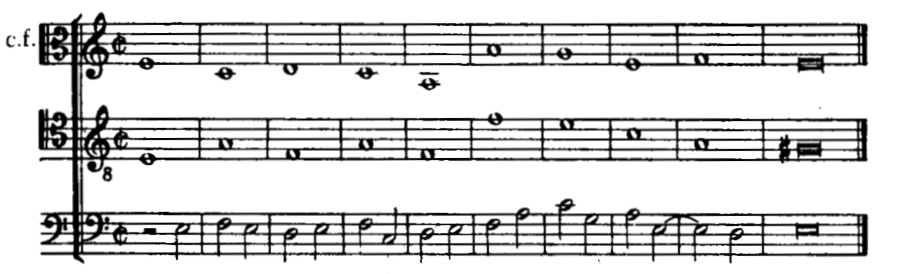
\includegraphics[width=1\textwidth]{Images/Species_examples/2sp-example.png}
    \caption{Example of a second species counterpoint in three-part composition}
    \label{fig:example-2sp}
\end{figure}
\subsection{Formalisation in English}\label{formalisation-en-2nd}
\subsubsection{Harmonic rules}
\begin{enumerate}[wide, label=\bfseries 2.H\arabic*]
\setcounter{enumi}{3} % Start from 4
    \item \textit{Major thirds are now allowed in the last chord.} \label{rule:major-third-last-chord}    
    \begin{quotation}
        "A major third [may] appear in the last chord."
        \textcite[p.87]{GaPEng}
    \end{quotation}
    This is a consequence of now using three voices instead of two. Fux makes explicit two implicit rules we had already defined (\ref{rule:last-chord-not-perfect-anymore} and~\ref{rule:last-chord-h-triad}). It has thus already been implemented in the first species for two voices.

    \item \textit{The half notes must be coherent with respect to the whole notes.} \label{rule:concur-2nd}    
    \begin{quotation}
        "The half notes are always concordant with the two whole notes."
        \textcite[p.88]{GaPEng}
    \end{quotation}
    One might ask what Fux meant when he wrote "concordant". Did he mean to say "consonant"? Our take on the question is that he meant that the half notes are written whilst taking the whole notes into account. This interpretation is aligned with the French translation, and even with the Latin original. In other words, Fux just says "there are constraints on the half notes". It is thus not a rule \textit{per se}.
\end{enumerate}

\subsubsection{Melodic rules}
\begin{enumerate}[wide, label=\bfseries 2.M\arabic*]
\setcounter{enumi}{1} % Start from 4
    \item \greendots \textit{It is allowed to ligate the fourth-to-last with the third-to-last or to ligature the third-to-last with the second-to-last.} \label{rule:2nd-species-ligatures}    
    \begin{quotation}
        "Ligatures have no place in this species [except] in the final cadence."
        \textcite[p.87]{GaPEng}
    \end{quotation}
    Fux explains that in some cases, you have no other option than ligaturing the fourth-to-last and the third-to-last notes. The reasons he gives for this are all part of the previous mentioned rules (no successive perfect consonances, no unison, ...).

    Later on, he also says that the third-to-last and the second-to-last notes can be ligatured (hence producing a whole note).
    \begin{quotation}
        "A whole note may occasionally be used in the next to last measure."
        \textcite[p.93]{GaPEng}
    \end{quotation}
    He says that in the chapter about third species, but it seems that this applies even in cases where the second species is not used in combination with the third (see figures 134, 173 and 174 of the English version).

    He doesn't state clearly if the three of them can get ligatured, but it seems quite obvious that this is not allowed, as it would introduce a lot of redundancy in the composition. It is hence decided that the rule is: a ligature may happen in one case or in the other, but not in both.

    We thus have to relax the already existing constraint from two-part composition stating that no two consecutive notes can be the same, to accept it in some cases.
\end{enumerate}

\subsubsection{Motion rules}
\begin{enumerate}[wide, label=\bfseries 2.P\arabic*]
\setcounter{enumi}{2} 
    \item \texttt{[PREF]} \textit{Successive fifths on the downbeat are only allowed when they are separated by a third on the upbeat.} \label{rule:succ-fifths-flanking-third}    
    \begin{quotation}
        "A half note may, for the sake of the harmonic triad, occasionally make a succession of two parallel fifth acceptable - which can be effected by the skip of a third."
        \textcite[p.86]{GaPEng}
    \end{quotation}
    Fux didn't speak about prohibiting two parallel (i.e. consecutive) fifths in the second species for two voices. That being said, it is indeed prohibited in three parts composition as you cannot have two successive perfect consonances (see rule~\ref{rule:succ-p-cons}). We thus have to relax constraint~\ref{rule:succ-p-cons} in order to accept two successive consonances, when the two successive fifths flank a third. And since the rule on successive perfect consonances is actually a preference, this means that the cost of successive perfect consonances is not applied if those two consonances are fifths and there is a third in between.

\vspace{.5cm}
\begin{minipage}{0.46\textwidth}
    \centering
    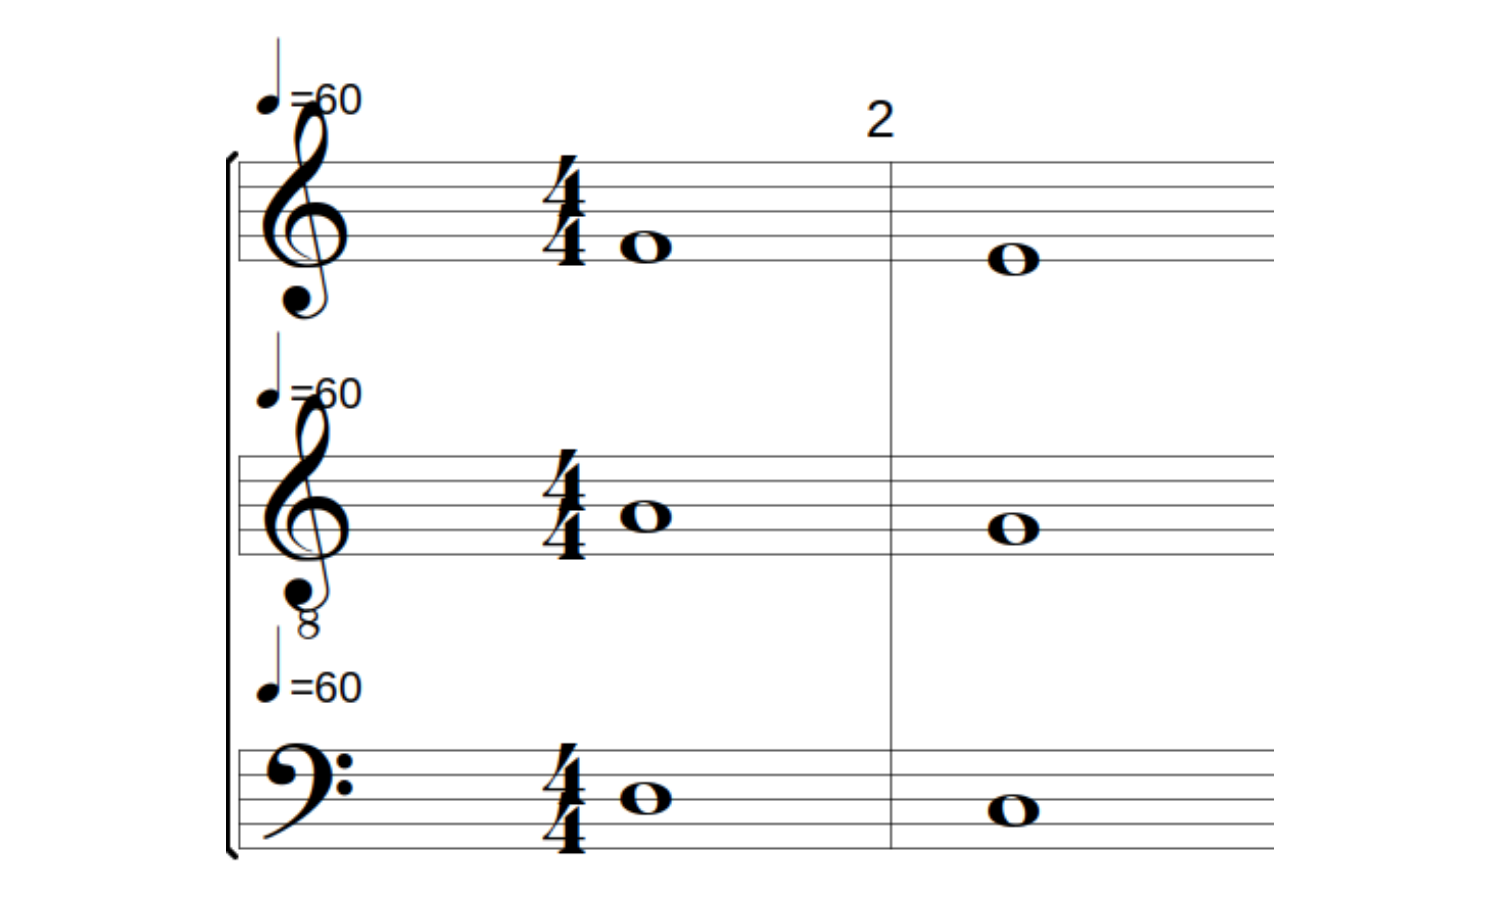
\includegraphics[width=\textwidth]{Images/successive-fifths.png}
    \captionof{figure}{Successive fifths - prohibited}
    \label{fig:successive-fifths-1}
    \end{minipage}
    \hfill
    \begin{minipage}{0.46\textwidth}
      \centering
      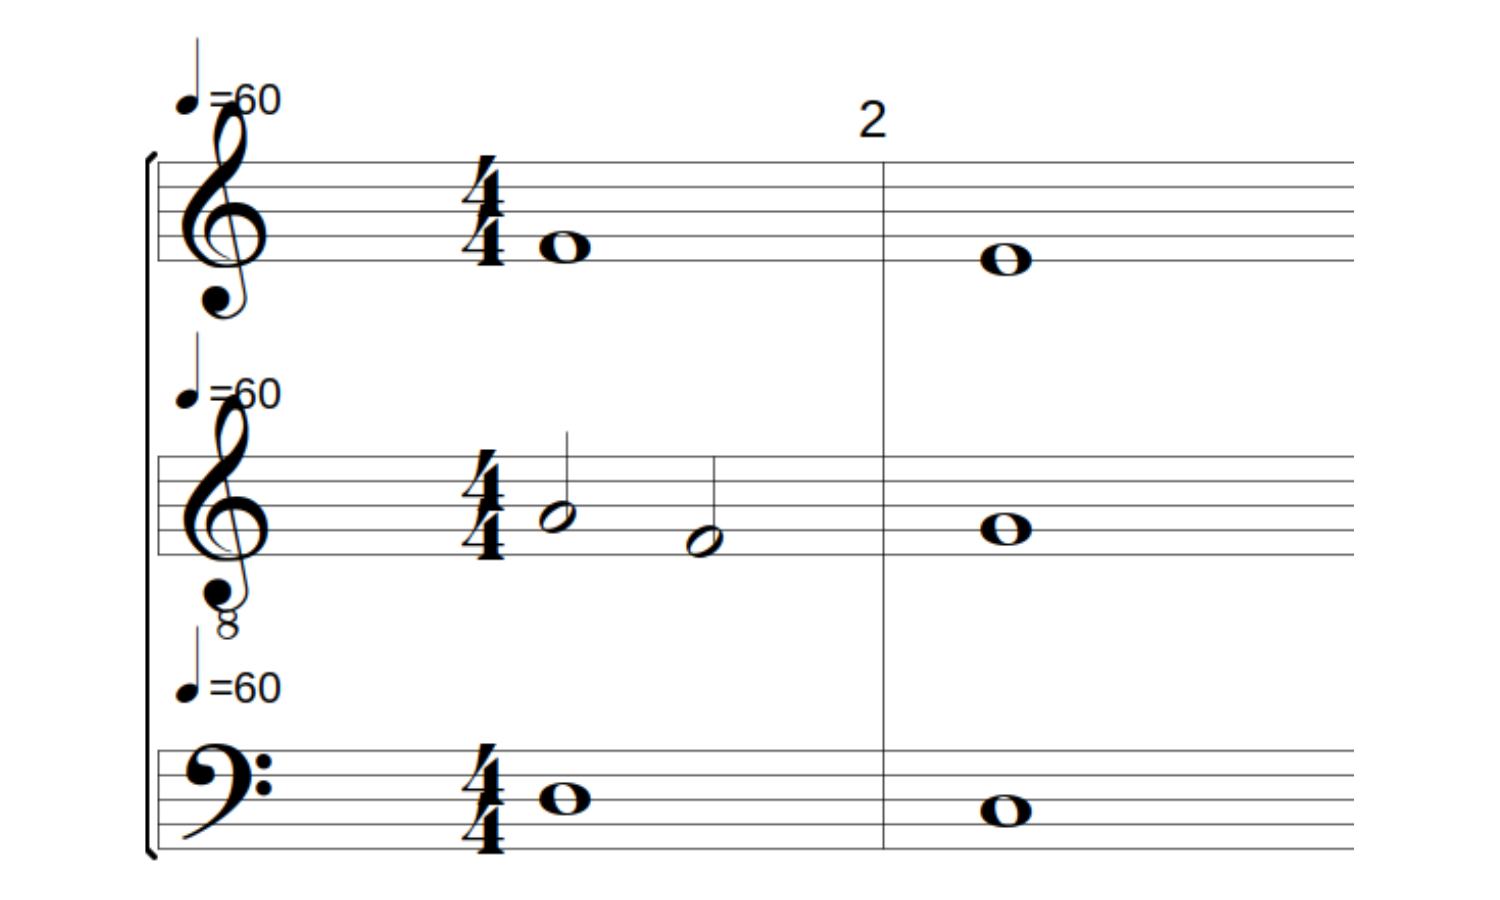
\includegraphics[width=\textwidth]{Images/successive-fifths-flanking-a-third.png}
      \captionof{figure}{Successive fifths separated by a third - valid}
      \label{fig:successive-fifths-2}
\end{minipage}
\end{enumerate}

\subsection{Formalisation into constraints}
\subsubsection{Harmonic rules}
\paragraph{\hspace{.5cm}\ref{rule:major-third-last-chord}} \textit{Major thirds are now allowed in the last chord.}

No need to add a new constraint as this rule is already covered by rules~\ref{rule:last-chord-not-perfect-anymore} and~\ref{rule:harmonic-triad}.

\paragraph{\hspace{.5cm}\ref{rule:concur-2nd}} \textit{The half notes must be coherent with respect to the whole notes.}

No need to add a new constraint as this is not an actual rule.

\subsubsection{Melodic rules}

    \paragraph{\hspace{.6cm}\ref{rule:2nd-species-ligatures}} \greendots \textit{It is allowed to ligate the fourth-to-last with the third-to-last or to ligature the third-to-last with the second-to-last.}  

    This is a relaxation of the two-voice rule \textbf{2.M2} "two consecutive notes cannot be the same".
    
    The reason why this rule has been implemented a constraint relaxation instead than as a cost is because Fux does not say that ligaturing is bad, he just presents it as a new option offered by the three-part composition.

    \begin{equation}
        \begin{aligned}
            &\forall j \in [1, m), \quad j \neq m-2:\\
            &((N[2, j-1] \neq N[0, j]) \land (N[0, j] \neq N[2, j])) \\
            &\land \\
            & ((N[2, m-3] \neq N[0, m-2]) \lor (N[0, m-2] \neq N[2, m-2]) )
        \end{aligned}
    \end{equation}

    The first line prohibits the ligatures except where on the positions where they are allowed, and the second line states that only one ligature can occur.

\subsubsection{Motion rules}
\paragraph{\hspace{.6cm}\ref{rule:succ-fifths-flanking-third}} \texttt{[PREF]} \textit{Successive fifths on the downbeat are only allowed when they are separated by a third on the upbeat.} 

    This rule is a relaxation of the cost~\ref{rule:succ-p-cons} defined above, and is thus rewritten to correspond to a special case that occurs with the second species.
        
    In the following equation, only $p_1$ must be a second species \cp, $p_2$ can be any species.
    \begin{equation}
        \begin{aligned}
            & \forall p_1, p_2 \in \{\mathit{cf}, cp_1, cp_2\} \text{ where }  p_1 \neq p_2, \quad \forall j \in [0, m-1): \\
            &\mathcal{C}_{succ\_p\_cons} = \,  
            \begin{cases}
                0 & \text{if } (H(p_1, p_2)[0, j] \notin Cons_p) \lor (H(p_1, p_2)[0, j+1] \notin Cons_p)\\
                0 & \text{if } (H(p_1, p_2)[0, j] = 7 ) \land (H(p_1, p_2)[0, j+1] = 7) \\
                & \quad \quad \quad \quad \quad \quad\land (H(p_1, p_2)[2, j] = 3) \lor (H(p_1, p_2)[2, j] = 4)\\
                2 & \text{otherwise } \\
            \end{cases}\\
        \end{aligned}
    \end{equation}

    The meaning of this equation is that $\mathcal{C}_{succ\_p\_cons}$ is equal to zero if one of the two considered consonances is not perfect (because then we do not have two successive perfect consonances), or if we have two successive fifths with a third in between. Otherwise (when we have perfect consonances), the cost must be set.

\section{Third species}
The second species consists only of quarter notes. It introduces even more dissonance than the second species and opens the space for more variation. 

All the rules in this section apply when $species(p) =3$. Note that the rules for the first species also apply to counterpoints of the third species.

\begin{figure}[h]
    \centering
    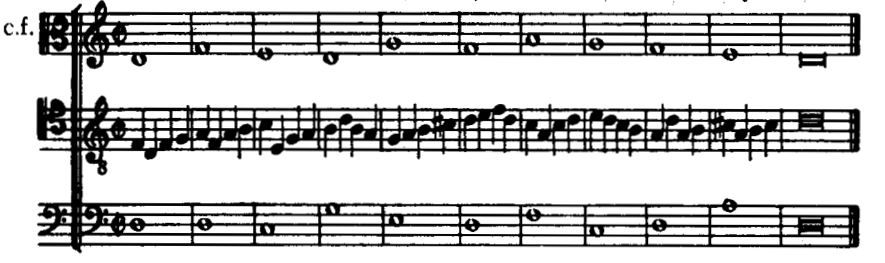
\includegraphics[width=1\textwidth]{Images/Species_examples/3sp-example.png}
    \caption{Example of a third species counterpoint in three-part composition}
    \label{fig:example-3sp}
\end{figure}
\subsection{Formalisation in English}\label{formalisation-en-3rd}
\subsubsection{Harmonic rules}
\begin{enumerate}[wide, label=\bfseries 3.H\arabic*]
\setcounter{enumi}{4}
    \item \textit{The quarter notes must be coherent with respect to the whole notes.} \label{rule:concur-3rd}    
    \begin{quotation}
        "The quarters have to concur with the whole notes of the other voices."
        \textcite[p.91]{GaPEng}
    \end{quotation}
    When using the word "concur", Fux more than probably means "are put in relation", and not "are consonant". As for rule~\ref{rule:concur-2nd} in the second species, where the half notes had to be \textit{concordant} with the \textit{cantus firmus}. It is not a rule by itself, Fux is only annunciating that some rules should be followed (i.e. the other constraints).

    \item\texttt{[PREF]}  \textit{If the harmonic triad could not be used on the downbeat, it should be used on the second or third beat.} \label{rule:h-triad-3rd-sp}     
    \begin{quotation}
        "Take care whenever you cannot use the harmonic triad on the first quarter occurring on the upbeat, to use it on the second or third quarters."
        \textcite[p.91]{GaPEng}
    \end{quotation}

    This rule is quite clear and speaks for itself.
\end{enumerate}

\subsubsection{Melodic rules}
Fux introduces no new melodic constraints for the third species.
\subsubsection{Motion rules}
Fux introduces no new motion constraints for the third species.

\subsection{Formalisation into constraints}
\subsubsection{Harmonic rules}
\paragraph{\hspace{.5cm}\ref{rule:concur-3rd}} \textit{The quarter notes must be coherent with respect to the whole notes.}
As has been discussed in the previous section, there is no constraint to add for this rule, which isn't really a rule.

\paragraph{\hspace{.6cm}\ref{rule:h-triad-3rd-sp}} \texttt{[PREF]} \textit{If the harmonic triad could not be used on the downbeat, it should be used on the second or third beat.}    

    This rule is quite clear and speaks for itself. Since this is not a strict rule but an advice, it was treated as a cost.

    \begin{equation} \begin{aligned}
            &\forall j \in [0, m) \colon \\
            &(H[1, j] \notin Cons_{h\_triad}) \land  (H[2, j] \notin Cons_{h\_triad})\\
            &\iff \mathcal{C}_{harmonic-triad-3rd-species}[j] = 1       
    \end{aligned} \end{equation}




\section{Fourth species}
As a reminder, the fourth species consists of syncopations. Each note is played on the upbeat and is ligated to the next note on the upbeat.

All the rules in this section apply when $species(p) =4$. Note that the rules for the first species also apply to counterpoints of the third species.

\begin{figure}[h]
    \centering
    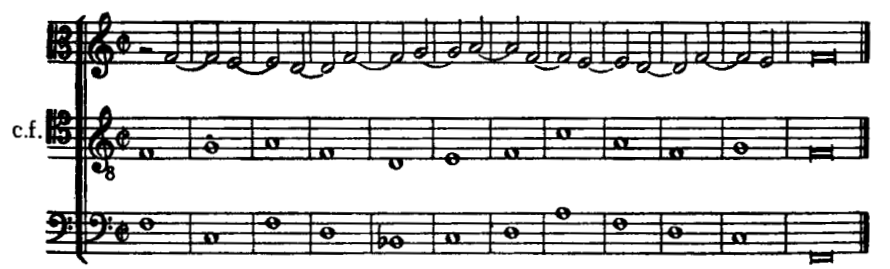
\includegraphics[width=1\textwidth]{Images/Species_examples/4sp-example.png}
    \caption{Example of a fourth species counterpoint in three-part composition}
    \label{fig:example-4sp}
\end{figure}

\subsection{Formalisation in English}\label{formalisation-en-4th}
\subsubsection{Structural constraints}
\begin{enumerate}[wide, label=\bfseries 4.S\arabic*]
\setcounter{enumi}{0}
    \item \textit{The fourth species is staggered by two beats.} \label{rule:delaying}    
    \begin{quotation}
        "The ligature is nothing but a delaying of the note following."
        \textcite[p.95]{GaPEng}
    \end{quotation}
    Fux here insists on a fact that we have already discussed in~\ref{nota-bene-4th-species}. The fourth species behaves as if its upbeat were the downbeat and its downbeat were the upbeat of the previous measure.

    \item \textit{All parts can become the lowest stratum somewhere in the composition.} \label{rule:tenor-might-take-place-of-bass}    
    \begin{quotation}
        "The tenor takes the place of the bass - a thing that not only the tenor may do, but also the alto and even the soprano."
        \textcite[p.100]{GaPEng}
    \end{quotation}
    Fux speaks here about our concept of strata. The tenor can become the lowest stratum, just like the alto and the soprano may do. This is a fundamental concept of the generalization of Fux counterpoint to three voices, and has already been extensively discussed before (see section~\ref{section:parts-and-strata}).
\end{enumerate}

\subsubsection{Harmonic rules}
\begin{enumerate}[wide, label=\bfseries 4.H\arabic*]
    \setcounter{enumi}{4}
    \item \texttt{[PREF]} \textit{Imperfect consonances are preferred over fifth intervals, which in turn are preferred over octaves.} \label{rule:prefer-fifths-over-octaves}    
    \begin{quotation}
        "The fifth is a perfect consonance, the octave a more perfect one, and the unison the most perfect of all; and the more perfect a consonance, the less harmony it has."
        \textcite[p.97]{GaPEng}
    \end{quotation}
    This rule is as clear as it gets.
\end{enumerate}

\subsubsection{Melodic rules}
Fux introduces no new melodic constraints for the third species.

\subsubsection{Motion rules}
\begin{enumerate}[wide, label=\bfseries 4.P\arabic*]
\setcounter{enumi}{2}
    \item \texttt{[PREF]} \textit{Successive fifths are allowed when using ligatures.} \label{rule:successive-fifths-in-4th-species}    
    \begin{quotation}
        "[It would be impossible to remove] the ligatures because of another consideration, the immediate succession of several fifths."
        \textcite[p.95]{GaPEng}
    \end{quotation}
    By saying that it exists a rule that prohibits the succession of fifths (which is actually just a particular case of rule~\ref{rule:succ-p-cons}, stating that you cannot have two successive perfect consonances) when there is no ligature, Fux is telling us in an indirect way that this rule is not applicable when there are ligatures. He further complements by saying "there is great power in ligatures - the ability to avoid or improve incorrect passages".
    
    The conclusion is that successive fifths are allowed in the fourth species.

    \item \texttt{[PREF]} \textit{Resolving to a fifth is preferred over resolving to an octave.} \label{rule:resolving-to-fifths-rather-than-octaves}    
    \begin{quotation}
        "A dissonance that resolves to a fifth is more acceptable than a dissonance that resolves to an octave."
        \textcite[p.98]{GaPEng}
    \end{quotation}
    This rule could not be clearer.
    
    \item \textit{Stationary movement in the bass implies dissonance in the fourth species part.} \label{rule:dissonance-in-4th-species}
    \begin{quotation}
        "If I said that the first note of the ligature must always be consonant, that applies only to the instances in which the lower voice moves from bar to bar, but not the instances in which the bass remains on a pedal point, that is, in the same position. In such a case a ligature involving only dissonances is not only correct but even very beautiful."
        \textcite[p.98]{GaPEng}
    \end{quotation}
    The rule evoked here cancels the previous rule \textbf{4.H1W} that stated that all notes should be consonant. From now on, if the lowest stratum has a stationary movement, the corresponding delayed note in the fourth species must be a dissonance, instead of a consonance.    


    \item \textit{A note provoking a hidden fifth gets replaced by a rest.} \label{rule:hidden-fifths}
    \begin{quotation}
        "Here a hidden succession of fifths occurs, which is easily perceptible to the ear and should be avoided in three part composition. This may be managed by using a rest."
        \textcite[p.98]{GaPEng}
    \end{quotation}
    Fux's uses the term 'hidden fifth' without any prior definition. It is therefore difficult to be sure of what he meant, since the traditional terms for such progressions are as vague and variable as the traditional rules that govern them. Nevertheless, most people seem to agree on the following definition of a 'hidden interval': a hidden fifth or hidden octave is when you approach a perfect fifth or perfect octave by direct motion. \cite[p.31]{piston1987harmony}. Looking closely at figures 137, 151 and 152 of the English version of \gap, this definition is consistent with Fux's interpretation.

    The point of the rule then is: if a solution leads to a hidden fifth, then the note that provokes the fifth is replaced by a rest. This rule is an \textit{a posteriori} rule: it applies after the solution has been found.
    The current rule thus complements the rule~\ref{rule:successive-fifths-in-4th-species} (about successive fifths in fourth species) and the rule~\ref{rule:direct-to-p-cons} (about direct moves to perfect consonances) without changing them.
    
    See figures~\ref{fig:hidden-fifths-1} and~\ref{fig:hidden-fifths-2}:

    \begin{figure}[h]
        \centering
        \begin{minipage}{0.49\textwidth}
            \centering
            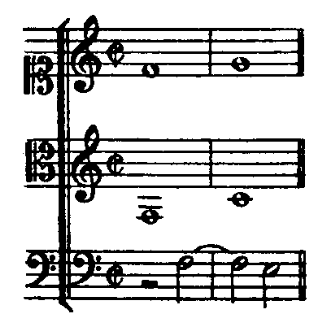
\includegraphics[width=.4\textwidth]{Images/hidden-fifths-1.png}
            \caption{Invalid solution featuring hidden fifths}
            \label{fig:hidden-fifths-1}
        \end{minipage}
        \hfill
        \begin{minipage}{0.49\textwidth}
            \centering
            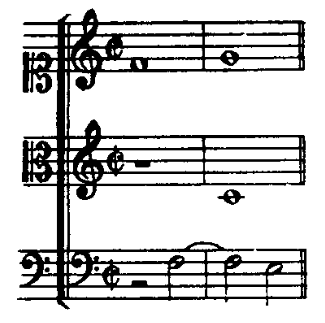
\includegraphics[width=.4\textwidth]{Images/hidden-fifths-2.png}
            \caption{Valid solution replacing the hidden fifth by a rest.}
            \label{fig:hidden-fifths-2}
        \end{minipage}
    \end{figure}

\end{enumerate}

\subsection{Formalisation into constraints}\label{formalisation-c-4th}
\subsubsection{Structural constraints}
    \paragraph{\hspace{.5cm}\ref{rule:delaying}} \textit{The fourth species is staggered by two beats.}

    There is no constraint to add since this rule is the very definition of the fourth species.

    \paragraph{\hspace{.5cm}\ref{rule:tenor-might-take-place-of-bass}} \textit{All parts can become the lowest stratum somewhere in the composition.} 
    
    Again, there is no constraint to add since this rule is already covered by the concept of lowest stratum.


\subsubsection{Harmonic rules}
\paragraph{\hspace{.6cm}\ref{rule:prefer-fifths-over-octaves}} \texttt{[PREF]} \textit{Imperfect consonances are preferred over fifth intervals, which in turn are preferred over octaves.}   

    This rule is almost covered by the existing costs (see~\ref{rule:prefer-imp-to-perf-appendix}), as a perfect consonance has a higher cost than an imperfect consonance. But Fux says not only that imperfect consonance should be preferred over perfect ones, he says that fifths should be preferred over octaves. This precision in the rule (fifth is better than octave) could be solved by either putting a higher cost to octaves and lower one to fifths, or to put the cost for fifth before the cost for octaves in the lexicographical array of costs, but this is discussed in the parts about costs (see~\ref{costs}).


\subsubsection{Motion rules}
In this subsection, the correct notation is used for the species (see \ref{nota-bene-4th-species}). So X[0,0] actually means X[0,0], and not X[2,0] as in other parts.

\paragraph{\hspace{.6cm}\ref{rule:successive-fifths-in-4th-species}} \texttt{[PREF]} \textit{Successive fifths are allowed when using ligatures.}    

    The point of this rule is that Fux introduces an exception to~\ref{rule:succ-p-cons}: successive fifths are allowed in the fourth species.

    We shall then amend the rule~\ref{rule:succ-p-cons} (don't forget that it is a cost) to allow successive fifths in any case, and rewrite it as:
    \begin{equation} \begin{aligned}
        &\forall p_1, p_2 \in \{\mathit{cf}, cp_1, cp_2\}, \quad \text{with } p_1 \neq p_2, \quad \forall j \in [0, m-1) \colon\\
        &\mathcal{C}_{succ\_p\_cons} = \,  
        \begin{cases}
            0 & \text{if } (H(p_1, p_2)[2, j] \notin Cons_p) \lor (H(p_1, p_2)[2, j+1] \notin Cons_p)\\
            0 & \text{if } (H(p_1, p_2)[2, j] = 7) \land (H(p_1, p_2)[2, j+1] = 7) \\
            2 & \text{otherwise } \\
        \end{cases}\\
    \end{aligned} \end{equation}

    The meaning of this equation is that the cost is set to zero if the two consecutive intervals are not perfect consonances, or if the consecutive intervals are both fifths. Otherwise, the cost must be set.

    \paragraph{\hspace{.6cm}\ref{rule:resolving-to-fifths-rather-than-octaves}} \texttt{[PREF]} \textit{Resolving to a fifth is preferred over resolving to an octave.}    
    
    This is already covered by the rule~\ref{rule:prefer-fifths-over-octaves} (prefer fifths over octaves), since preferring fifths over octaves in \textit{all} cases implies preferring to resolve to a fifth rather than to an octave.

    \paragraph{\hspace{.6cm}\ref{rule:dissonance-in-4th-species}} \textit{Stationary movement in the bass implies dissonance in the fourth species part.}

    \begin{equation}
        \begin{aligned}
        &\forall j \in [0, m-1):\\
        &M(a)[0, j] \neq 0 \iff H[2, j] \in Cons\\
        &M(a)[0, j] = 0 \iff H[2, j] \in Dis
        \end{aligned}
    \end{equation}        


    \paragraph{\hspace{.6cm}\ref{rule:hidden-fifths}} \textit{A note provoking a hidden fifth gets replaced by a rest.}
    \begin{equation}
        \begin{aligned}
            &\forall j \in [1, m-1):\\
            &H[0, j] = 7 \land P[0,j] = 2 \iff N[0, j-1] = \emptyset  
        \end{aligned}
    \end{equation}

    This rule is very special because it applies after the search, not during the search. More precisely, after the search is started and a result is found, only then does this rule begin to apply. To understand why, remember that the suppressed note is suppressed because it causes a hidden fifth. But the only way to have a hidden fifth is to have an existing note, you cannot have a hidden fifth to a non-existing note. So we don't delete the note during the search, because then we would also delete the hidden fifth (because you can't have a hidden fifth without a note) and so we would change the solution. You have to find a solution first, and then remove the possible note that causes a hidden fifth. 

    This is actually a very interesting property, because here we have a note that is not played and yet has an effect on the composition.



\section{Fifth species}

As a reminder, the fifth species is a mix of all previously mentioned species, which means that it combines the rules from all previous species.

\begin{figure}[h]
    \centering
    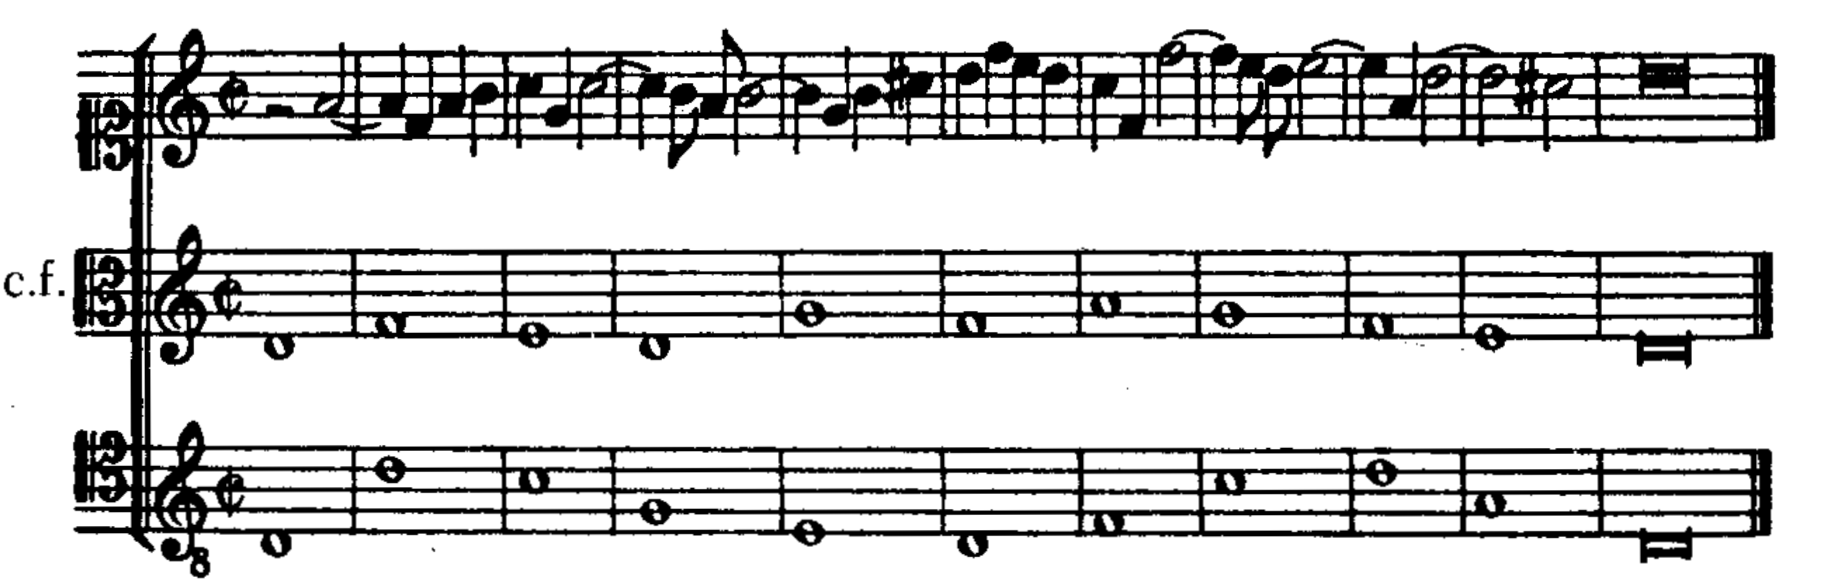
\includegraphics[width=1\textwidth]{Images/Species_examples/5sp-example.png}
    \caption{Example of a fifth species counterpoint in three-part composition}
    \label{fig:example-5sp}
\end{figure}

\paragraph{}
No additional rules (be they harmonic rules, melodic rules or motion rules) were observed by Fux when writing a three-part counterpoint with the fifth species.


However, in order to have some rhythmic variety when composing with two fifth species counterpoints, it was decided to impose a rule that Fux never mentioned. We know that the fifth is just all the other species combined, and the way the solver understands this is that it considers each note of the composition to belong to a particular species. This is represented as S[i,j], where $S[i,j]=x$ means that the i-th note of the j-th measure belongs to the x-th species. So if $S(cp_1)[2, 3]=3$, then the second note of the third measure of the first counterpoint is constrained by the constraints of the third species. From the solver's point of view, $S$ is just an array like all the others, but it branches on it during the search to guarantee that the composition of the fifth species is composed of as many species as possible.

This gives us a metric for similarity, since two fifth-species counterpoints that have the same $S$ array will be rhythmically redundant. To tackle this problem, we force the solver to find a solution where $S(cp_1)$ must be at least half as different as $S(cp_2)$. 

\noindent
\begin{minipage}{0.37\textwidth}
    As can be seen in Figure \ref{fig:fifth-species-redundancy}, the first composition is indeed rhythmically redundant, since both fifth-species counterpoints have (almost) the same rhythm. The second is much less redundant, since it was required that the counterpoints use different species for at least 50\% of the beats.
    \end{minipage}
    \hfill
    \begin{minipage}{0.6\textwidth}
      \centering
      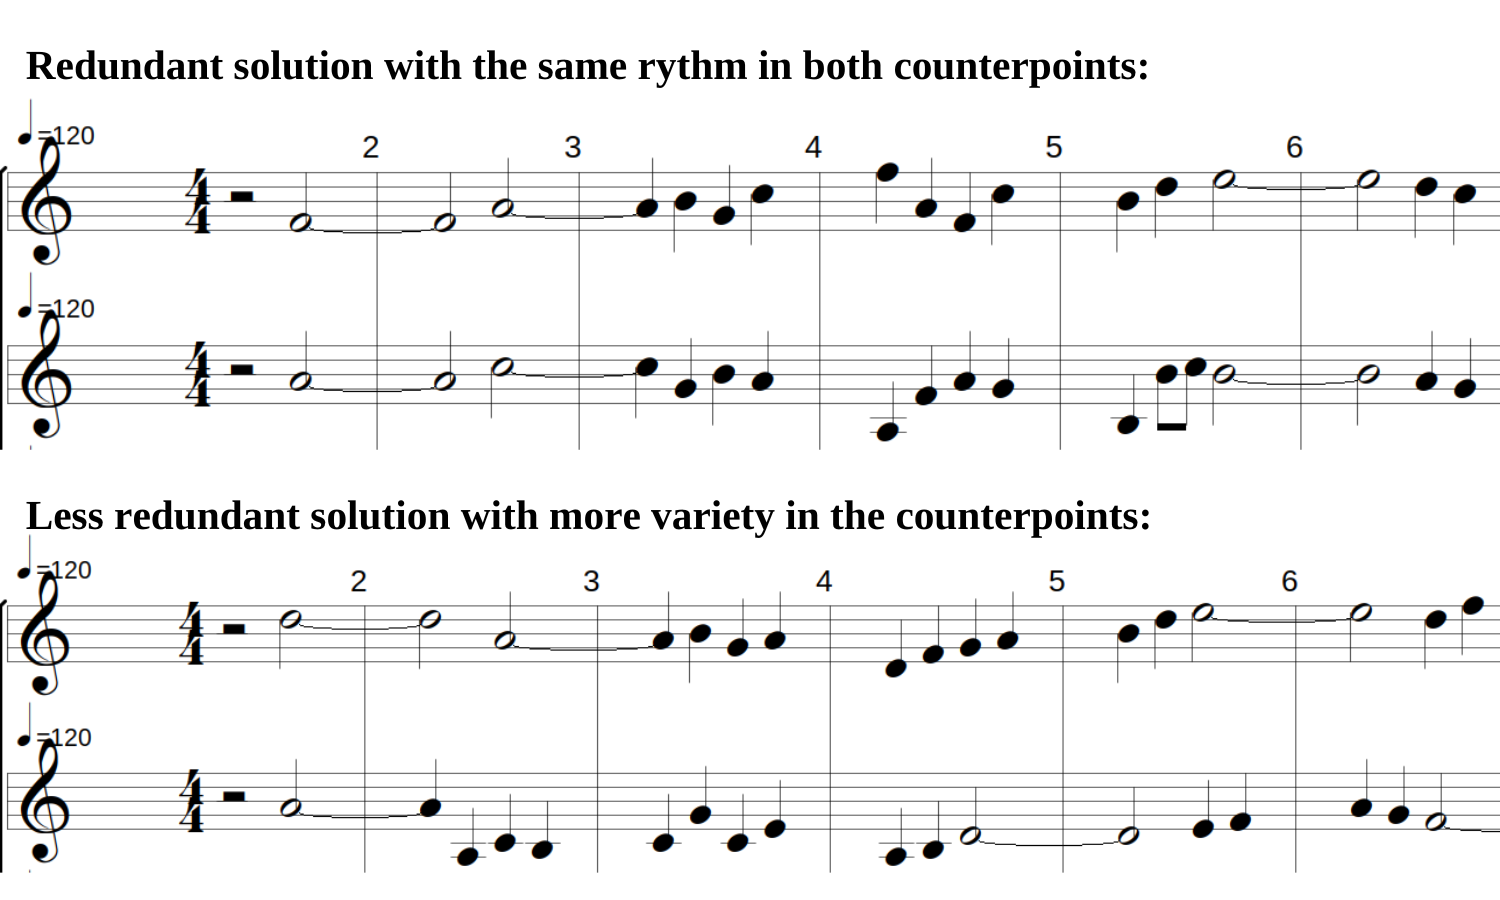
\includegraphics[width=\textwidth]{Images/fifth-species-redundancy.png}
      \captionof{figure}{Two compositions of two fifth-species counterpoint, one redundant and the other not}
      \label{fig:fifth-species-redundancy}
\end{minipage}
\vspace{.5cm}


\begin{equation}
\begin{aligned}
 \mathit{species(cp_1)} = \mathit{species}(cp_2) = 5 \iff \sum_{i=0}^{3} \sum_{j=0}^{m-1} (S(cp_1)[i,j] = S(cp_2)[i,j]) < \frac{s_m}{2}
\end{aligned}
\end{equation}

This equation is only true if both counterpoints are of the fifth species, and its meaning is that the sum of the times $S(cp_1)=S(cp_2)$ must be less than half the number of notes in the composition.

\section{Writing a three-part composition using various species}
In \gap, Fux almost always writes his counterpoints using a combination of the first species and another species, i.e. he makes the following combinations: 1+1, 1+2, 1+3, 1+4, 1+5. Only sometimes does he make other combinations, either with two counterpoints of the same type (5+5) or with two different types (2+3).

When creating combinations of different species, Fux doesn't give any specific rules for combining them. It seems that the different species interact with each other as they would do with the first species, taking into account only the first beat of the measure. For example, if we compute a first counterpoint belonging to the 3rd species and a second counterpoint belonging to the second species, the rules that apply between the two counterpoints will be set between all the beats of the first counterpoint and the first beat of the second counterpoint and between all the beats of the second counterpoint and the first beat of the first counterpoint. This corresponds to what we would have done if we had applied the rules between a counterpoint and the \cf, where the rules apply between all beats of the \cfs and the first beat of the counterpoint.

Below is a brief summary of the rules that apply to each species:
\begin{itemize}
    \item \textbf{First species} --- rules of the first species,
    \item \textbf{Second species} --- rules of the first species + rules of the second species,
    \item \textbf{Third species} --- rules of the first species + rules of the third species,
    \item \textbf{Fourth species} --- rules of the first species + rules of the third species,
    \item \textbf{Fifth species} --- rules of all species, selected according to the S array.
\end{itemize}
This means that in a composition with two counterpoints, one of the 2nd species and one of the 3rd species, the first counterpoint will follow the rules of the 1st and the 2nd species, and the second counterpoint will follow the rules of the 1st and the 3rd species.
\chapter{Searching for the best existing solution}
Three parts composition brings in way more possibilities than two parts composition. 
But more possibilities also mean an increased computation complexity. The search space has been extended a lot by adding a whole new set of variables, and the time taken for a solution to be found might to be too elevated if one does not think about optimizing the search. In addition to that, adding a third voice to a composition is not bringing many new constraints (which would help discarding some potential solutions faster), but instead comes with many preferences, which in constraint programming, are translated to costs.

In addition, we need to find a way of arranging the costs in a way that comes as close as possible to what Fux was trying to express in his book. There are several ways to do this, which we will go through and discuss.  

This chapter will begin by explaining the search algorithm that is used to find a solution, continue by discussing the different ways of considering costs, and end by analysing the results that these different perspectives produce.

\section{Using Branch-And-Bound as a search algorithm}

To cope with the increased complexity brought about by the three-part composition, it was decided to switch from the Depth First Search algorithm (used in T. Wafflard's thesis) to a more efficient Branch and Bound (BAB). This allows us to handle costs properly and to find faster solutions. Moreover, the BAB algorithm can also produce non-optimal results, which is very valuable since finding the best overall solution can be time-consuming. When starting the search for a solution, it is now possible to ask for the next solution (i.e. a better solution than the one found previously, and if none was found previously, then just any valid solution), or for the best solution. In the latter case, the solver will continue to search until it finds the best solution or until it is stopped, returning a better solution each time it finds one.


\subsection{Heuristics} \label{heuristics}
\subsubsection{Main heuristics}
When it comes to finding a solution, we obviously need some heuristics to guide the search, as there are so many different possibilities for a three-part composition. 
To know which heuristics to use, simply think about the most important variable to fix first. In case it is not clear enough, the key to writing counterpoint for many voices is to know what the bass is doing. This is true whether the composer is a human or a constraint solver. So the first heuristic follows naturally, and it is: branch on the lowest stratum array, take the highest constrained variable yet, and try with its lowest possible value.


The other central heuristic is the one that instructs the solver to branch on the variables of the $N$ arrays (containing the pitches of the voices), choosing as a priority the variables whose domain is small. This choice is motivated by the fact that in the case of a highly constrained counterpoint (5th species) and a weakly constrained counterpoint (1st species), the counterpoint should not only seek to improve the highly constrained counterpoint, but also the weakly constrained counterpoint. This is why the heuristic chosen is based on the size of the domain and not on the level of constraint. The choice of the value of the variable is then random. This ensures maximum diversity in the final composition and quickly leads to a solution whose notes are varied.


\subsubsection{Additional heuristics}
A first additional heuristic is to branch to the array representing the species contained in the fifth species, to ensure a varied composition. If we are dealing with a counterpoint of the fourth or fifth species, we also branch on the "no ligature cost", so that the solver explores solutions in which the notes are linked, since this is the very nature of the fourth species (both when it is used "pure" and when it is used within the fifth species).

The rule \ref{rule:start-distant} states that the voices should start distant, and as suggested in the section on rules, this should be implemented in a heuristic. However, when we implemented the heuristic that all voices should start distant from the lowest one, we did not see any improvement, neither in search speed nor in solution quality. In fact, it sometimes slowed down the search, so this heuristic was dropped. Furthermore, Fux's advice that the voices should start far apart in order to progress in the opposite direction is only true if the bottom layer moves up. If the bottom stratum moves down, the top strata should move up, so starting far apart becomes a compositional disadvantage in this case (as the voices are limited by their range).



\subsection{Time to find a solution} \label{section:time-to-find-a-solution}
Many factors come into play in determining how long it will take the solver to find a valid solution. These factors are mainly: the species of counterpoints, the spacing between the voice ranges of the counterpoints, and the key of the \cf.


In general, the solver is able to find a valid solution fairly quickly (in the order of a second). In some cases, however, it cannot find a valid solution (and so searches endlessly). These cases are generally related to the three factors mentioned above, and we will discuss them a little. Each of these factors makes the search a little more difficult. A single factor may have no effect on the search time, and it is sometimes at the intersection of the factors that an effect is discovered.

\begin{itemize}
    \item \textbf{Species of the counterpoint} \textendash{} The more complex the species of the counterpoints (think of the 3rd and 5th species, for example), the longer it will probably take the solver to find a solution. The reason is quite obvious: the more complex the species, the more variables the solver has to play with and the greater the range of possibilities.  
    \item \textbf{Distance between the voice ranges} \textendash{}  The closer the ranges of the voices, the greater the risk that the solver will take a long time to find a solution. For example, finding a solution by giving the two counterpoints the same voice range as the \cfs is more time-consuming than selecting distant voice ranges. This is because the voices cannot form a unison, and the possibilities for each voice are therefore smaller when their range is close together. 
    \item \textbf{Key of the \cf} \textendash{} The solver finds it much easier to find a counterpoint when the key is C, probably because counterpoints are played with as many natural notes as possible (no flats or sharps), and in the case of C this corresponds to the Ionian mode (also known as the C mode). When using the key of X, the further away the X mode is from the C mode, the more difficult it will be for the counterpoint. For example, take a composition in E: the E (Phrygian) mode is far from the C (Ionian) mode, whereas the G (Myxolydian) mode is quite close. The solver will therefore find it slightly more difficult to find a solution in E than in G, which in turn will be more complicated than in C.
\end{itemize}
There are also cases where the exact combination of two given vocal ranges for two given species with a given mode does not give a solution, but by changing the vocal range a little the solver finds a solution immediately, quite surprisingly. It is still unclear why some given combinations do not produce solutions. Our best guess is that there are some combinations of parameters for which the solver has difficulty finding a solution, given the very large number of constraints that apply to the voices. However, this doesn't happen very often.

It is worth noting that the solver's greatest difficulty (in all cases) is finding a valid solution. Once a valid solution has been found, the solver quickly finds a whole series of solutions, each one better than the previous one (until, of course, it is difficult to find the best solution).


\section{Designing the costs to be as faithful as possible to \gap} \label{costs}

Knowing that we are looking for the solution whose cost must be as low as possible, the question arises: how can we calculate the cost in order to best reflect the preferences expressed in \gap?

The way to translate each preference into a corresponding cost has of course been formalised in the previous sections, but that's not the crux of the matter. The question we face here is: what is the best way to combine all these individual costs to get the most accurate result in terms of what Fux is trying to convey?

Three main ways of doing this have been identified: a linear combination between costs, a search that minimises costs by lexicographic order, and a cost ordering that involves the calculation of minima. We will first describe each of these techniques and their respective advantages, and then compare them (and the results they produce).



\subsection{Linear Combination}


The first method of calculating our costs is a linear combination. This is the technique used in T. Wafflard's thesis. More precisely, it uses a linear combination in which all the weights are equal to one.



To be more precise about the method used to calculate the total cost in T. Wafflard's thesis, here is a more detailed explanation: there exists a total cost, $\tau$, which is equal to the sum of all individual costs, $\mathcal{C}$. The next step is to minimise $\tau$. Each $\mathcal{C}_i$ is usually itself a sum of sub-costs. Take, for example, the cost of motions, $\mathcal{C}_{motions} = \sum_j P_{costs}[j] $. This cost is the sum of all sub-costs of the motions (one per motion): by default, a contrary motion has a sub-cost of 0, an oblique motion has a sub-cost of 1 and a direct motion has a sub-cost of 2. These default values can be changed by the user to be set somewhere on a scale that ranges from $0$ to $64m$. For example, the user could set the oblique motion cost to be equal to $0$, and the cost for direct and contrary motion to be equal to $64m$, in order to get a composition filled with as many oblique motions as possible (always in accordance with the basic rules from \gap, i.e. all voices are never going to go in the same direction, see \ref{rule:same-movement}).

As mentioned at the beginning of this subsection, this procedure can be understood as a linear combination with weights of one only. However, since the cost factors are given different values according to the user's choices, this method is actually more like a regular linear combination, except that the weights are not multiplied by the costs once the latter have been set, but the costs are themselves made larger or smaller before the linear combination is calculated.

The linear combination has two major advantages: ease of implementation and high comprehensibility.


However, it has a major drawback: since the total cost $\tau$ we are minimising in a linear combination is the sum of all costs $\mathcal{C}$, the best solution might be a solution where one cost is absolutely huge and all the others are small. This might not be a problem if the outstanding cost is not really relevant, but if it is the cost of not using a harmonic triad, it goes completely against the preferences that Fux conveys in his work, making the solution inappropriate. A representation of this situation can be found in the figure \ref{fig:outstanding-cost}.

\begin{figure}[h]
    \centering
    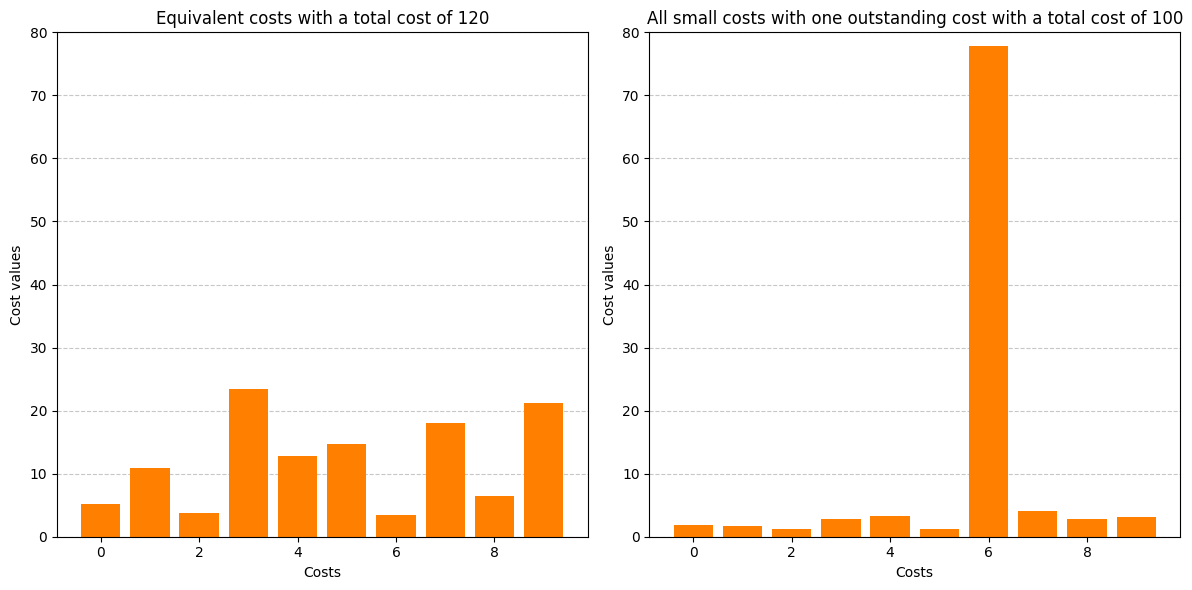
\includegraphics[width=1\textwidth]{Images/outstanding-costs.png}
    \caption{Example of a situation where a solution with an outstanding cost is preferred to a solution with equivalent low costs when using a linear combination}
    \label{fig:outstanding-cost}
\end{figure}

Another drawback of linear combination is that the result is pretty and unpredictable: changing the value of the cost may or may not make a difference, and you may need to set huge values to see a real effect. For example, if a composer really wants oblique motion, they may be forced to set the cost of the other types of motion to a huge value, or they may not see the difference between the default solution and their personalised solution. This is due to the fact that all the costs are mixed together and form an indistinguishable soup that the solver considers as a whole, and a small increase in the cost of the direct and contrary motions is very likely to be absorbed into this soup without any change being noticed.

These two drawbacks make the linear combination solution for the costs hardly acceptable when it comes to representing the preferences.
We will therefore examine the other two options for adjusting costs.

\subsection {Minimising the maxima} \label{section:minimising-the-maxima}
In order to overcome the problem of outstanding costs that we encountered when considering the linear combination solution, one might consider using some minimums when calculating $\tau$, the total cost. For example, $\tau$ could be the maximum of all costs. By doing this, the solver would try to find a solution where the focus is on the worst cost and try to reduce it before trying to reduce the other costs.

The problem with this method arises when one cost is significantly higher than the others because it has been defined that way. Let's go back to our example of the composer wanting as many oblique motions as possible. You will set the cost for direct motion and contrary motion to the highest possible cost and start the search. As we've already discussed, it is not possible to have only oblique motions, since this would contradict the rule that not all voices can move in the same direction (\ref{rule:same-movement}). As a result, there will always be contrary motions, and since the cost for them has been set very high, it would be impossible for the solver to converge to a good solution. This creates a bottleneck effect, where once the solver has reached the best potential value of the worst cost, it cannot continue to find better solutions. 

\begin{figure}[h]
    \centering
    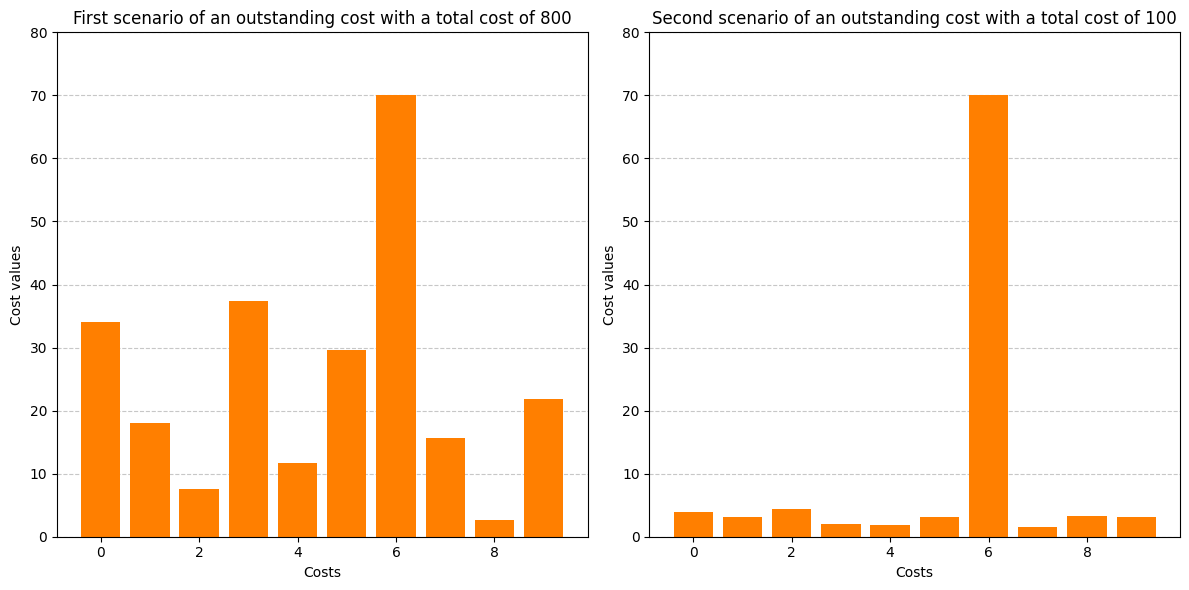
\includegraphics[width=1\textwidth]{Images/minimising-maxima.png}
    \caption{Example of two situations where a cost causes a bottleneck in the search because the solver cannot distinguish between left and right situations. The solver will blindly choose one of the two solutions, even if the solution on the left is obviously better.}
    \label{fig:bottleneck}
\end{figure}


Furthermore, even when considering a less extreme case (e.g. the default setting), this method requires a normalisation of the costs: there are $3\times (m-2)$ sub-costs for the variety cost, $3\times (m-1)$ sub-costs for the motion cost, but only $m$ sub-costs for the octave cost. This means that without normalisation, the motion cost will be on average three times larger than the octave cost, which means that the solver will put three times more effort into minimising the motion cost than the octave cost, which is unfair and unpractical.


\subsection{Lexicographical Order}\label{section:lexicographical-order}
The second way of dealing with the costs is to arrange them in an array and then perform a lexicographic minimisation. In other words, the costs would be arranged in order of importance: from most important to least important. The most important cost to minimise would be placed first in this array, and the solver would only try to minimise the other costs if the first cost remained the same or decreased. This method makes a lot of sense when you think about the rules that emanate of \gap. For example, Fux says that perfect consonance can be achieved by direct motion if there is no other possibility. This means that, all other things being equal, we would prefer to achieve perfect consonance by oblique or contrary motion, but that between a bad solution (respecting almost no preferences) in which perfect consonance is not achieved by direct motion, and a good solution (respecting almost all preferences) in which perfect consonance is achieved by direct motion, we would choose the good solution. 

Some costs are also more important than others in absolute terms. For example, when Fux says that an imperfect consonance is preferred to a fifth, which is preferred to an octave. This amounts to lexicographically ranking the cost of using an octave first (because we really don't want octaves), and then the cost of using a fifth (and there is no cost of using an imperfect consonance, since Fux indicates that this is preferable).
\begin{figure}[h]
    \begin{equation}
        \begin{aligned}
            \tau = [\underset{\text{minimise this first}}{\underbrace{\mathcal{C}_\text{octaves}}}, \mathcal{C}_\text{fifths}]
        \end{aligned}
    \end{equation}
    \caption{Array of costs demonstrating the practicality of a lexicographical order solving.}
\end{figure}

A second example, which ties in particularly well with the first, is that Fux tells us that the harmonic triad must be used in every measure unless a rule forbids it. In saying this, he places the preference for the harmonic triad above all other preferences, because the only reason that can prevent the use of a harmonic triad is a fixed constraint (and not a preference). You'll notice that the harmonic triad consists of a fifth (which is a perfect consonant), so Fux is telling us that we'd rather use a fifth in a harmonic triad than an imperfect consonant outside a harmonic triad. The lexicographic order search is the only one that allows this kind of concept to be taken into account, because in a linear combination these two preferences would be mutually "exclusive"\footnote{In the sense that their effects would work against each other.}: the first preference would add a cost where the second preference would not, and the second preference would add a cost where the first would not.

\begin{figure}[h]
    \begin{equation}
        \begin{aligned}
            \tau = [& \underset{\text{\fontsize{7}{11}\selectfont{minimize this first}}}{\underbrace{\mathcal{C}_\text{harmonic\_triad}}}, \underset{\text{\fontsize{7}{11}\selectfont\parbox{4cm}{and start minimizing this only if it is not possible anymore to minimize the harmonic triad cost}}}{\underbrace{\mathcal{C}_\text{octaves}}},\quad  \mathcal{C}_\text{fifths}]
        \end{aligned}
    \end{equation}
    \caption{Array of costs demonstrating the practicality of a lexicographical order solving.}
\end{figure}

And in this way we can keep integrating the different costs until we get a full array $\tau$ with all the costs ordered in a lexicographical way.


Of course, it is not always as simple as in the examples above, because it is not always easy to determine which cost has priority over which other. Sometimes Fux is very clear about it (e.g. for the harmonic triad cost, which Fux says has priority over everything else), and sometimes he isn't (do we prefer no off-key notes, or as much variety as possible?) This is a drawback of this method, because we have to hierarchise the costs, even if the choice is difficult. What's more, once the costs are ranked, their order becomes absolute and the solver loses some of its flexibility.


Knowing this, we came up with a suggested order that should be as close as possible to Fux's preferred order (or at least what we understood him to convey as his preferred order in \gap). This order should of course be changeable at the composer's discretion. The default order we have agreed upon is as follows. Please note that where a cost is followed by a number in brackets, this means that it only applies if the corresponding species is used.
\begin{multicols}{2}
    \begin{enumerate}
        \item $\mathcal{C}_\text{no\_syncope}$\footnote{The cost of not using a syncope.} [4, 5] 
        \item $\mathcal{C}_\text{successive\_p\_cons}$
        \item $\mathcal{C}_\text{harmonic\_triad}$
        \item $\mathcal{C}_\text{harmonic\_triad\_3rd\_species}$ [3]
        \item $\mathcal{C}_\text{octaves}$
        \item $\mathcal{C}_\text{penult\_thesis\_is\_fifth}$\footnote{A specific cost for the second species, which applies when a penultimate thesis note does not make a fifth interval with the lowest stratum.} [2]
        \item $\mathcal{C}_\text{fifths}$
        \item $\mathcal{C}_\text{off\_key}$\footnote{The cost of using sharps or flats.}
        \item $\mathcal{C}_\text{variety}$
        \item $\mathcal{C}_\text{m2\_eq\_zero}$\footnote{The cost of having the same note in the downbeat and the upbeat.} [3, 4, 5]
        \item $\mathcal{C}_\text{not\_cambiata}$\footnote{The cost of not using a \textit{cambiata} if it is possible. The \textit{cambiata} can be characterised by the following scheme: \texttt{consonance - dissonance - consonance}.} [3, 5]
        \item $\mathcal{C}_\text{motions}$
        \item $\mathcal{C}_\text{m\_degrees}$\footnote{The cost of using big or small melodic intervals.}        
        \item $\mathcal{C}_\text{direct\_move\_to\_p\_cons}$
    \end{enumerate}
\end{multicols}

Some notes on the proposed order: 
\begin{itemize}
    \item Two costs come even before the harmonic triad cost: the $\mathcal{C}_\text{no\_syncope}$ cost and the $\mathcal{C}_\text{successive\_p\_cons}$ cost. Regarding the $\mathcal{C}_\text{no\_syncope}$ cost: this cost is at the heart of the fourth species, and a fourth species counterpoint without syncopations is not really a fourth species counterpoint. This is why syncopation is considered even more important than the harmonic triad. And concerning the $\mathcal{C}_\text{successive\_p\_cons}$ cost: when Fux expresses his preference for the harmonic triad, he says that there are reasons that are even more important (see rule \ref{rule:harmonic-triad}), and not having successive perfect consonances is one of them.
    \item The cost of $\mathcal{C}_\text{penult\_thesis\_is\_fifth}$ comes before the cost of $\mathcal{C}_\text{fifths}$, as it is an exception to the latter (similar to the interaction explained above in the section between $\mathcal{C}_\text{harmonic\_triad}$ and $\mathcal{C}_\text{fifths})$.
    
    \item $\mathcal{C}_\text{off\_key}$ was added to its ranking because it is actually an absolute rule not to use off-key notes, but Fux does use some, and so it was decided to put this cost after the very important costs to allow off-key notes to happen.

    \item The costs $\mathcal{C}_\text{variety}$, $\mathcal{C}_\text{motions}$ and $\mathcal{C}_\text{m\_degrees}$ were ranked in order from least to most restrictive. First we say that we would prefer the note to change as much as possible (with the variety cost), then we indicate our preference for the direction (with the motion cost), and finally we indicate our preference for the size of the motion (with the melodic interval cost). This gives the solver as much flexibility as possible. The other way round would have been more restrictive, since the solver would have minimised the melodic intervals first, setting them all to one, which doesn't leave much room for the motion cost to have an effect, and forcing the variety cost to be high in any case, as with  intervals the melody tends to vary only a little.
    
    \item $\mathcal{C}_\text{m2\_eq\_zero}$ and $\mathcal{C}_\text{m\_degrees}$ were classified right after the variety cost as they are an in-measure variation of the variety preference.

\end{itemize}


\paragraph{NB} Please note that using the lexicographic order does not \textit{not} mean that the last costs are not taken into account, they will be \textit{too} minimised by the solver. It just means that if the solver has to choose between minimising one cost or another, it will minimise the first one in the lexicographic order. 

\subsection{Comparison between the three types of costs.}

We have now discussed the advantages and disadvantages of each of the three methods. These are all listed in \ref{tab:comparison}. As you can see, no one method is definitively better than another, and the only way to know which method is better in practice is to \textit{test} them in practice to find out which of the methods gives the best results. 

\begin{center}
    \centering
    \captionof{table}{Comparison of Three Methods According to Criteria}
    \label{tab:comparison}
    \begin{tabularx}{\textwidth}{|>{\centering\arraybackslash}p{4cm}|>{\centering\arraybackslash}X|>{\centering\arraybackslash}X|>{\centering\arraybackslash}X|}
        \hline
        \textbf{Criteria} & \textbf{Linear Combination} & \textbf{Minimising the maximum} & \textbf{Lexicographic Search} \\
        \hline
        Outsanding costs & \cellcolor{red!25}Yes & \cellcolor{green!25}No & \cellcolor{orange!25}Only for minor costs \\
        \hline
        Sensitivity\footnote{In the sense that changing one cost has a big impact on the result.} & \cellcolor{red!25}No & \cellcolor{orange!25}Some & \cellcolor{green!25}Yes \\
        \hline
        One cost might be a bottleneck & \cellcolor{green!25}No & \cellcolor{red!25}Yes & \cellcolor{green!25}No \\
        \hline
        Need to normalise costs& \cellcolor{green!25}No & \cellcolor{red!25}Yes & \cellcolor{green!25}No \\
        \hline
        Possibility to ensure a preference of one cost over another  & \cellcolor{red!25}No & \cellcolor{red!25}No & \cellcolor{green!25}Yes \\
        \hline
        Need for hierarchisation of costs & \cellcolor{green!25}No & \cellcolor{green!25}No & \cellcolor{red!25}Yes \\
        \hline
        Flexibility & \cellcolor{orange!25}Medium & \cellcolor{green!25}High & \cellcolor{red!25}Low \\
        \hline

    \end{tabularx}
\end{center}

Even more, one could think about a combination of all the methods to get rid of their disadvantages. In fact, we could enjoy the advantages of all the methods by combining them and cleverly designing a lexicographical order search in which the cost is a linear combination of a maximum minimisation.

\subsection{Experimenting with the three types of costs arrangements}
To experiment which method gives the best results, we will follow this plan: first compare the result of a linear combination and the result of a purely lexicographical order, using the default preference order as defined in \ref{section:lexicographical-order}. We then analyse the result by looking at what could have been done to manage costs more effectively and, where appropriate, group costs together.


These experiments are carried out using two different counterpoint combination setups. These setups will increase in complexity, starting with the basic case of 3-voice counterpoint (two counterpoints of the 1st species) and moving on to mixed counterpoints. 

The advantage of simple species (first, second and fourth species) is that the search for a solution is much faster. In fact, the search for an optimal solution can be quite time-consuming, and this is even more the case when we are talking about complex species such as the third and the fifth, and when they are combined. This means that it is more difficult to grasp the impact of the cost method when using a setup with complex species. What's more, the vast majority of the costs are related to the interaction of the voices in the first beat of the measures: the behaviour we want to observe, i.e. the interaction between the cost method and the resulting composition, will be just as observable with complex species as with simple ones. Having said that, we are still going to test the cost arrangement methods on all species.

The analyses in this section are superficial and do not deal with in-depth music theory. They will consist of general surface and impression remarks. They are highly subjective and should not be taken at face value. The aim of this analysis is to provide an initial critical view of the results offered by the solver.

The selected \textit{cantus firmi} were chosen from \gap. If the search time exceeds 30 seconds, the search is stopped and the current solution is analysed.
\subsubsection{First experiment: two first-species counterpoints on two different \textit{cantus firmi}}
\begin{figure}[h]
    \centering
    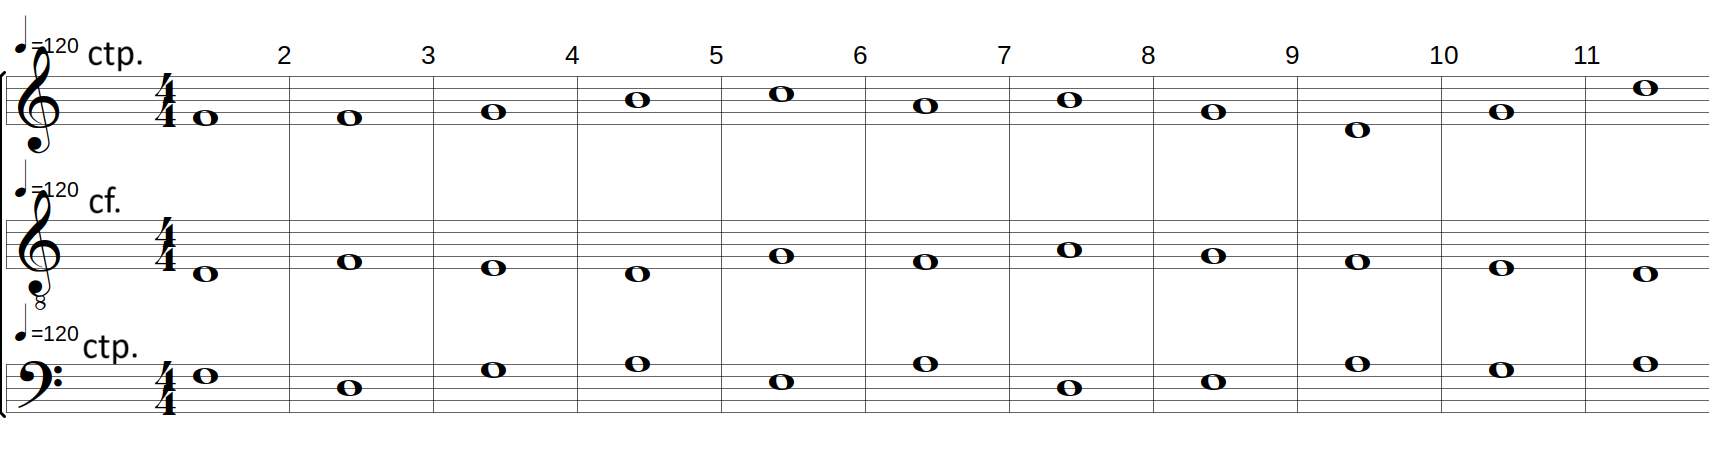
\includegraphics[width=1\textwidth]{Images/Experiments/linear-combination-1sp.png}
    \caption{Result 1 of the linear combination method with default costs.}
    \label{fig:combili-1sp}
\end{figure}

\begin{figure}[h]
    \centering
    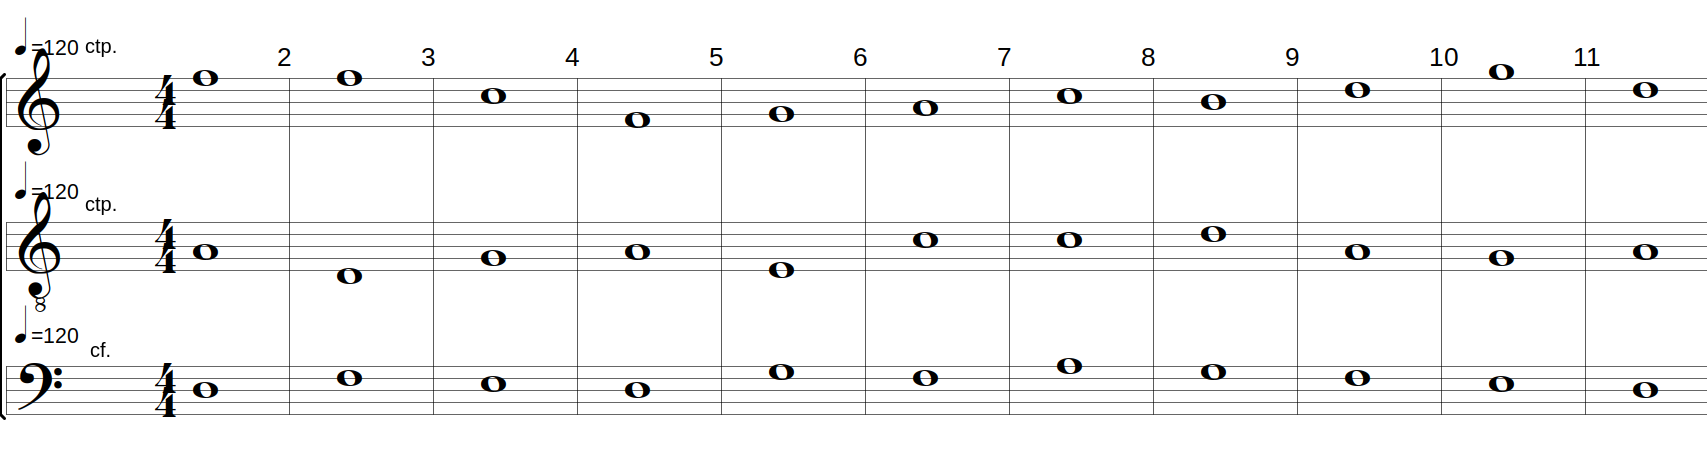
\includegraphics[width=1\textwidth]{Images/Experiments/basic-lexico-1sp.png}
    \caption{Result 1 of the lexicographic search method with default costs.}
    \label{fig:lexico-1sp}
\end{figure}

% above very far above
Here are the first two results: \ref{fig:combili-1sp} and \ref{fig:lexico-1sp}. To the average ear, there's not much difference between these two solutions, except that the second is perhaps a tad more vibrant. The linear combination solution feels like chords that follow one another without any discernible link between them, whereas the solution with the lexicographical order offers a solution that seems to hold together better over time. What's more, the linear combination solution contains a few dissonances that are not so pleasing to the ear.

In more technical terms, the two solutions are fairly similar, and both feature the same number of harmonic triads, i.e. one, which is a really small number given the eleven measures of the composition. The lexicographic solution is composed of four direct motions, whereas the linear combination solution only is composed of only three. However, the solution does not suffer from any particular redundancy to the ear, as you do not get the impression of hearing the same melody three times. The lexicographic composition gives a more melodic impression than the composition by linear combination.

\begin{figure}[h]
    \centering
    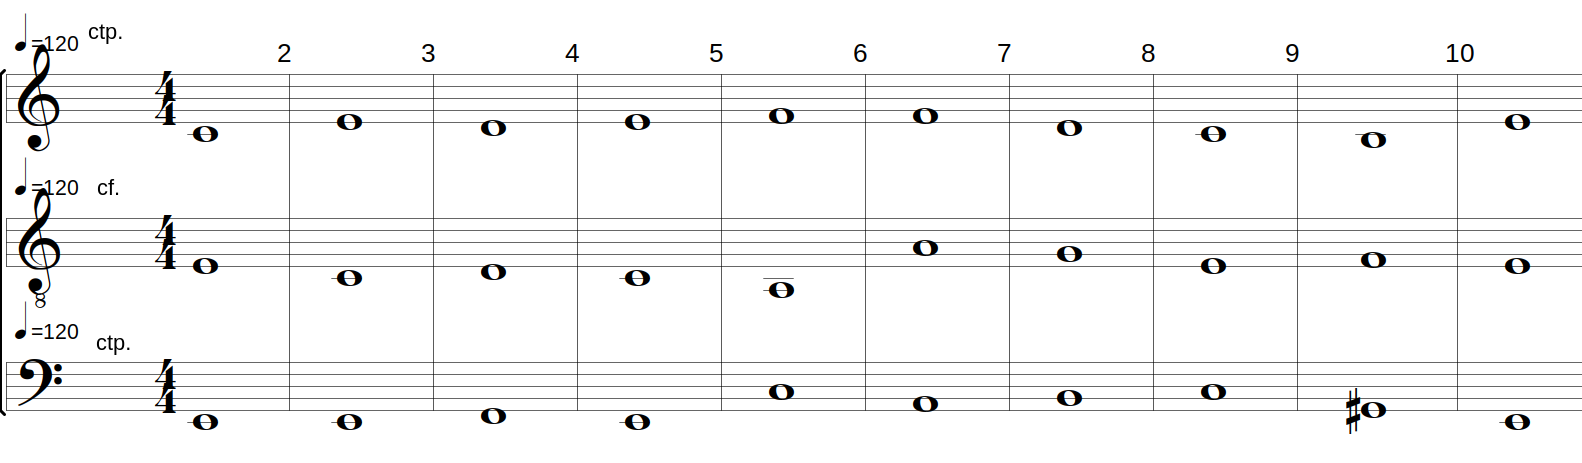
\includegraphics[width=1\textwidth]{Images/Experiments/linear-combination-1sp0.png}
    \caption{Result 2 of the linear combination method with default costs.}
    \label{fig:combili-1sp0}
\end{figure}

\begin{figure}[h]
    \centering
    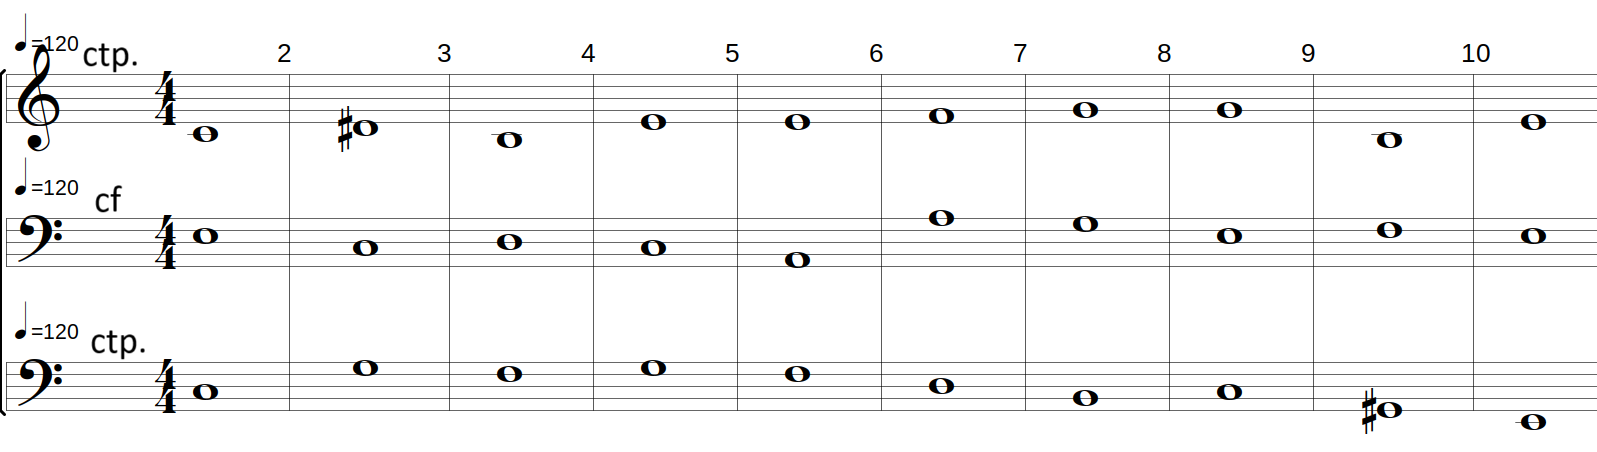
\includegraphics[width=1\textwidth]{Images/Experiments/basic-lexico-1sp0.png}
    \caption{Result 2 of the lexicographic search method with default costs.}
    \label{fig:lexico-1sp0}
\end{figure}

% below far above
Let's look at the second result (obtained with a different \cf), featured in figures \ref{fig:combili-1sp0} and \ref{fig:lexico-1sp0}. Once again, there's no major difference between the two solutions, although once again the linear combination solution seems to lack a melodic direction. The dissonances are more numerous and once again it feels like a series of unrelated chords. In contrast, and perhaps it's a coincidence, but the solution proposed by the lexicographical research seems to tell a dark story.

Once again, the technical results are fairly similar: two harmonic triads for the linear combination and three for the lexicographical search. Again, this is surprisingly few, given that there are ten measures in the composition. Both solutions feature four direct motions, but one does not feel a lack of independence of the voices in any of them.

Now what happens when we start to mix the techniques and group some of the costs in the lexicographic order? At each level of the lexicographic order, we calculate the maximum of the costs at that level, which we then try to minimise. All preferences that Fux has not explicitely ordered get packed on the same level, i.e. three levels subsist: the first one, with only the cost for successive perfect consonances, the second one, with only the cost for not using a harmonic triad, and a third one, with all the other costs.

\begin{figure}[h]
    \centering
    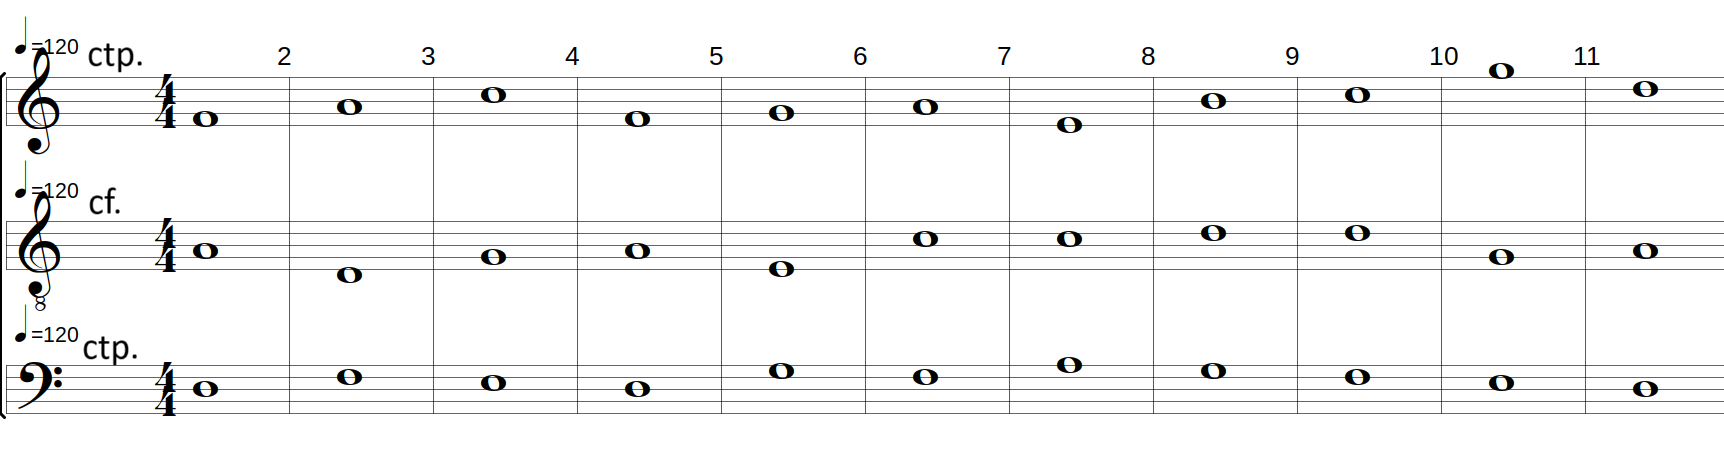
\includegraphics[width=1\textwidth]{Images/Experiments/min-1sp.png}
    \caption{Result 1 of a mix between lexicographic and maximum minimisation method.}
    \label{fig:min-sp}
\end{figure}
\begin{figure}[h]
    \centering
    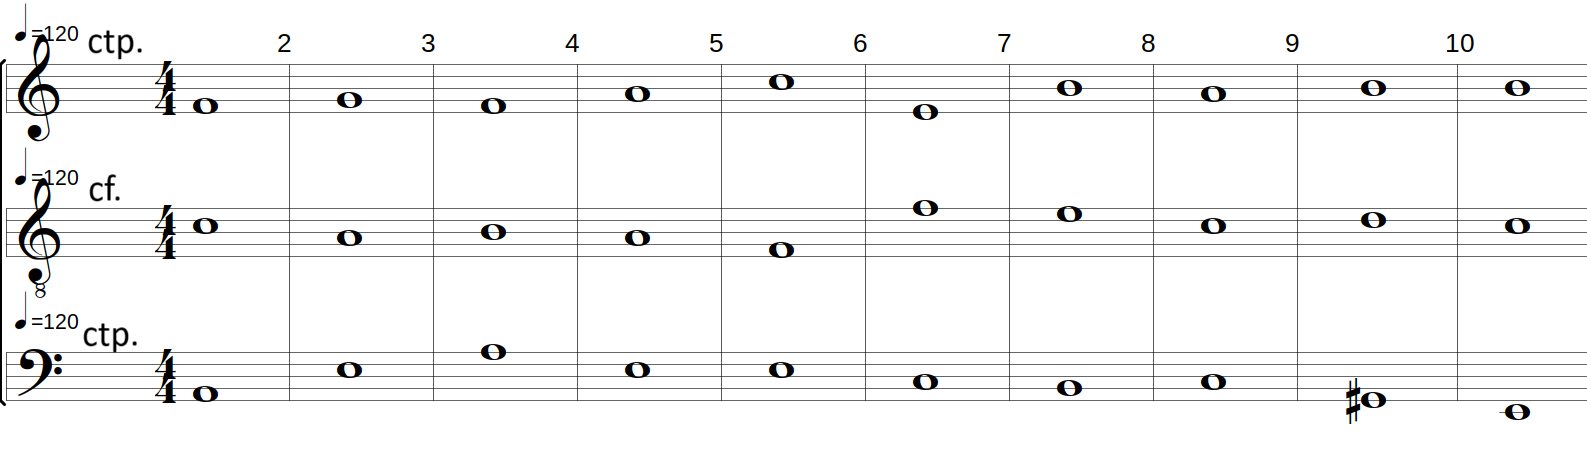
\includegraphics[width=1\textwidth]{Images/Experiments/min-1sp0.png}
    \caption{Result 2 of a mix between lexicographic and maximum minimisation method.}
    \label{fig:min-sp0}
\end{figure}

Figures \ref{fig:min-sp} and \ref{fig:min-sp0} show the solutions found by mixing the techniques of lexicographic order and maximum minimisation.

Both solutions handle the ending strangely, but this may be a coincidence, as there is no cost that would obviously cause such an ending.

It would be too bold to say that there is a big difference between the results obtained by this method and those obtained by the others. In other words, to the average ear, the solutions provided by this search technique are not significantly different from those provided by the other search methods.


The good news, however, is that the result, far from being excellent, is different. This means that a composer can set up the tool as they wish and get different results from one setup to another. They might start with the default settings and then change one parameter after another until they find what suits them best. This is really good news, because it means that the solution is not too limited to a few possibilities, but that once a valid solution has been found, there is still too much room for personalisation!


Note that the predicted bottleneck effect from section \ref{section:minimising-the-maxima} was indeed observed in both searches, as the solution stopped improving after only ten seconds of search. After these ten seconds, the solver stopped finding better solutions because the third cost level (the one whose maximum was minimised) had already reached its minimum maximum, and so the solver could not distinguish between two solutions if they had the same maximum, since this search technique doesn't allow it. Please refer to figure \ref{fig:bottleneck} for a better understanding of the situation.

The following can be concluded from these initial experiments
\begin{enumerate}
    \item The lexicographic order seems to give results with a stronger sense of coherence: the composition seems to tell a story (to a very limited extent, of course).
    \item Linear combination gives more dissonant results.
    \item The three search methods give three different results, so a composer could experiment.
    \item Our view of the best search method so far is: there is none. The best that can be done is to use a mixture of lexicographical order and maximum minimisation, with personalised orders, to find a counterpoint that the composer will like.
\end{enumerate}
\subsubsection{Second experiment: one fourth-species counterpoint and one first-species counterpoint on a single \cf}

If we now go on, here is a result combining the first and the fourth species, and putting the 4th species at the bottom:
\begin{figure}[h]
    \centering
    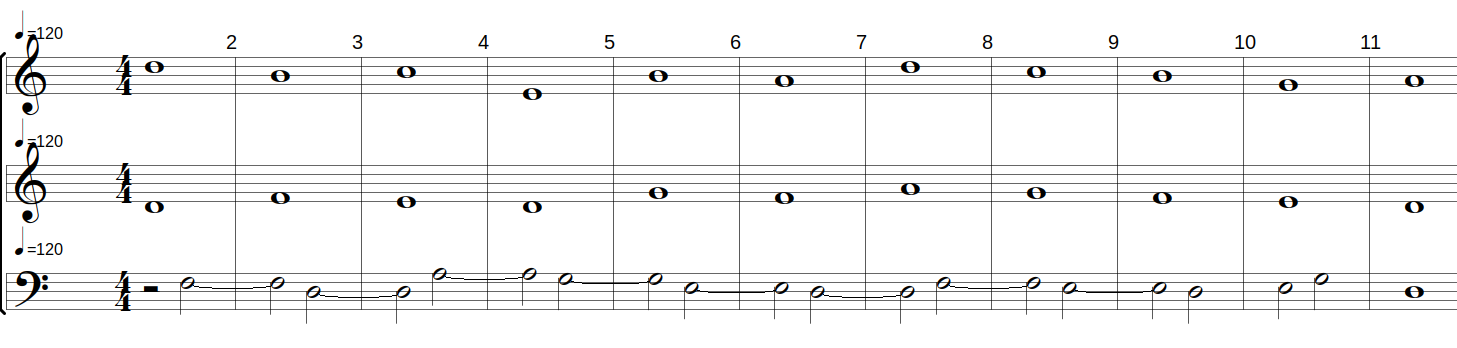
\includegraphics[width=1\textwidth]{Images/Experiments/linear-combination-4sp.png}
    \caption{Result 3 of the linear combination method with default costs.}
    \label{fig:combili-4sp}
\end{figure}

\begin{figure}[h]
    \centering
    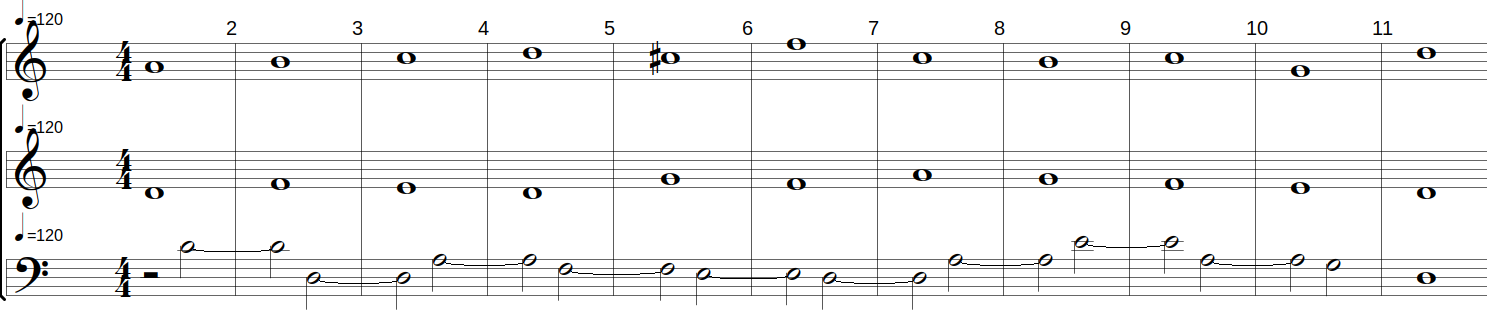
\includegraphics[width=1\textwidth]{Images/Experiments/basic-lexico-4sp.png}
    \caption{Result 3 of the lexicographic search method with default costs.}
    \label{fig:lexico-4sp}
\end{figure}
Looking at the results obtained with this setup (figures \ref{fig:combili-4sp} and \ref{fig:lexico-4sp}), we come to the same conclusions as in the previous experiment. 
In both cases, the melody is a little dull and lacks dynamism. There is no drastic change in quality between the solutions provided by the two search techniques. However, the solution provided by the lexicographic search is somewhat more exciting, since there is more tension in it and it uses more dissonances and resolvings than the linear combination (even if these resolvings are not the most brilliant).

We immediately notice something else with the 4th species on the bass, which is not related to the costs: there are a few dissonances on the downbeat, as the solver doesn't really take into account the harmonic interaction between the notes of the downbeat of the fourth species and the notes of the downbeat of the other species, but rather the harmonic interaction between the upbeat of the fourth species and the downbeat of the others: which leads to a few surprises, as we can see in these examples (that tension mentioned above).

As far as the costs are concerned, one thing is clear: not all the notes of the 4th species obtained with a linear combination are linked, whereas they all are in the solution of the lexicographic order. This is an obvious consequence of using a linear combination, as this technique is not able to prioritise a cost.


\subsubsection{Third experiment: one third-species counterpoint and one second-species counterpoint on a single \cf}
Our first cross-species test will involve a counterpoint of the 2nd species and a counterpoint of the 3rd species. The \cfs used is the one proposed by Fux in an example in which he uses exactly these two species. The search was given one minute, as the complexity is getting higher than in the previous experiments.


The results are shown in the figures:

\begin{figure}[h]
    \centering
    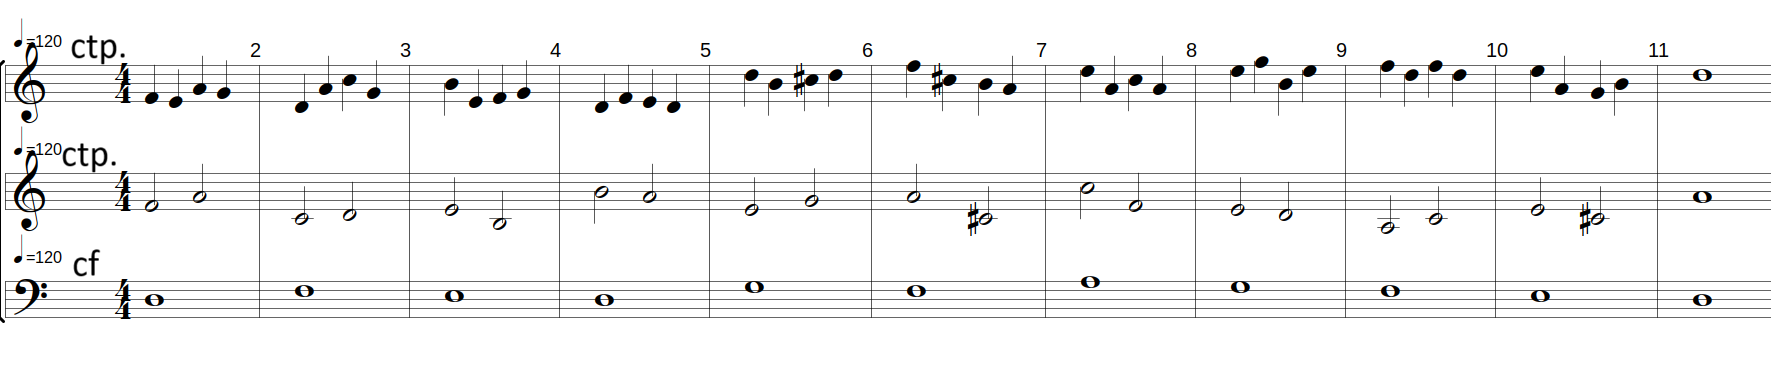
\includegraphics[width=1\textwidth]{Images/Experiments/linear-combination-2sp.png}
    \caption{Result 4 of the linear combination method with default costs.}
    \label{fig:combili-2sp}
\end{figure}

\begin{figure}[h]
    \centering
    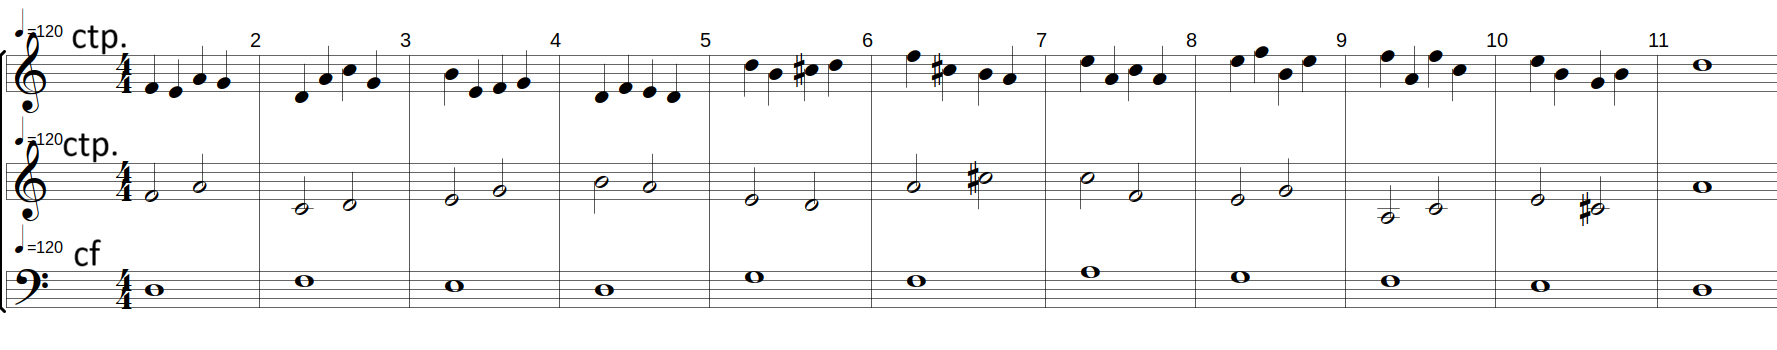
\includegraphics[width=1\textwidth]{Images/Experiments/basic-lexico-2sp.png}
    \caption{Result 4 of the lexicographic search method with default costs.}
    \label{fig:lexico-2sp}
\end{figure}

The results are strikingly similar. And unmelodic. Let's look at these two aspects in turn.


About the similarity: The similarity is probably due to two things: the solver doesn't have much room for manoeuvre, since all the voices are highly constrained, so the costs don't have much of an effect in this very setup. 

Concerning the lack of melodic quality: it is probably due in part to bad luck (this \cfs is perhaps particularly difficult to handle) and in part to the lack of constraints linking the upbeats of the various counterpoints. If you think about it, all the rules proposed by Fux in his chapter on three-voice composition link the beats of one voice (\textit{all its beats}) to the first beat of the other voices. This means that there are constraints between the 2nd, 3rd and 4th beats of one voice and the other voices, but never between these 2nd, 3rd and 4th beats of one voice and the 2nd, 3rd and 4th beats of another voice, always with the 1st beat. Obviously, without rules to ensure that the notes of these beats concur\footnote{The word 'concur' is used here in the same sense that Fux uses it: it means that the notes are somehow put in a relationship that makes them sound good together.}, it is more complicated for these beats to concur. Of course, it would be wrong to say that it depends only on chance that these beats concur, because that would mean that the beats are independent. Indeed, one might think so at first, because there are no constraints directly linking them, and yet they are linked by their own connections with the first beat of the other voices. In other words, although the third beat of the first counterpoint is not directly linked to the third beat of the second counterpoint, it is indirectly linked to it through the first beat of the second counterpoint: there are constraints between this third beat of the first counterpoint and the first beat of the second counterpoint, and there are also constraints between the first beat of the second counterpoint and the third beat of the second counterpoint. There is therefore a certain dependency and mutual influence between the 3rd beats of the two counterpoints. However, it would be interesting to see if Fux introduces any rules on this subject in his chapter on four-part composition, and if not, it would be interesting to think about what these rules might be in order to maximise the concordance between the notes in the upbeat of the different voices.
\subsubsection{Fourth experiment: two fifth-species counterpoints}
The fourth experiment is a bit special, as it features two fifth counterpoints \textit{with the same voice range}. This is something Fux doesn't really do in \gap, but we thought it might be interesting to see how the search method behaves in this situation. Even though Fux doesn't write counterpoints in the same voice range, they are still realistic, for example in the case of a double violin concerto, or any other instrument that has the same voice range and that is played together.

In this experiment, it is interesting to observe how the solver manages the small margin of manoeuvre it has, given that it has to find two counterpoints in the same voice range, all when the counterpoints are forbidden to take the same value (i.e. the same pitch).

The search was run for two minutes instead of thirty seconds, as the fifth species counterpoint is more complex than the others, and a little more time is needed to let the costs have an effect on the solution. The solutions are those in figures \ref{fig:combili-5sp} and \ref{fig:combili-5sp}.

\begin{figure}[h]
    \centering
    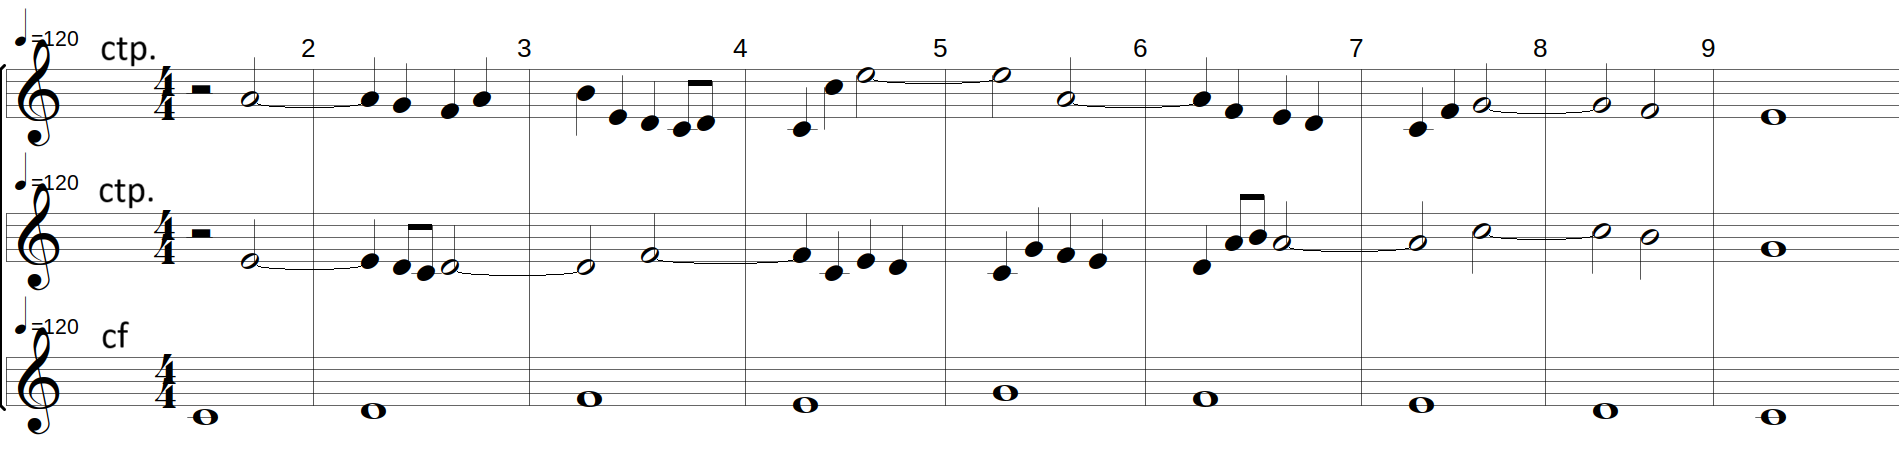
\includegraphics[width=1\textwidth]{Images/Experiments/linear-combination-5sp.png}
    \caption{Result 5 of the linear combination method with default costs.}
    \label{fig:combili-5sp}
\end{figure}

\begin{figure}[h]
    \centering
    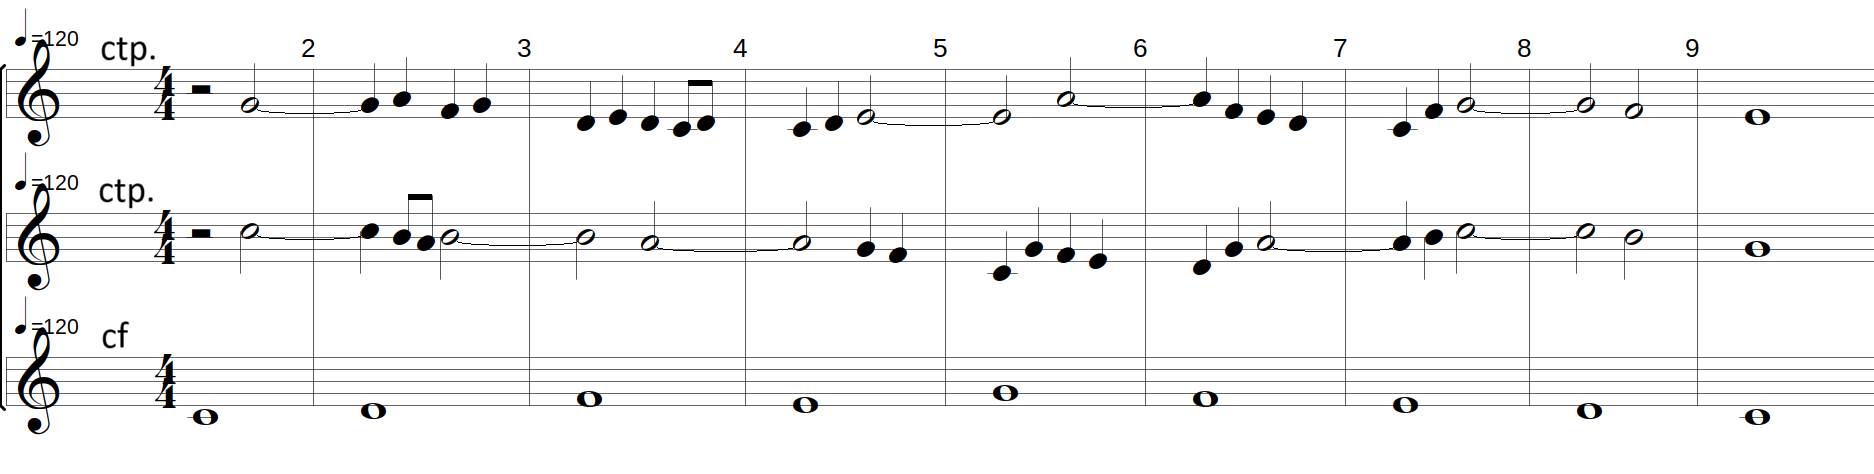
\includegraphics[width=1\textwidth]{Images/Experiments/basic-lexico-5sp.png}
    \caption{Result 5 of the lexicographic search method with default costs.}
    \label{fig:lexico-5sp}
\end{figure}

Just as for the second experiment, some interesting things happen in the composition found by the lexicographic search. The intervals are more beautiful and the fact that there are dissonances that sometimes resolve gives more meaning to what's going on.

On the other hand, the fact that the penultimate note of the middle voice resolves on a G instead of a C is a bit frustrating, as the final chord feels like it is not a real ending, but this is a recurring problem in all solutions. The reason for this is probably that there is a rule (rule \ref{rule:prefer-fifths-over-octaves}) that makes the solver prefer fifths to octaves, and there is no mention from Fux of deviating from this rule for the last measure.

\textit{However}, the solver did a surprisingly good job of finding passable solutions with such a small search field. The solutions obtained are far from high art, but you can see the musical intuition behind them.

\subsubsection{Conclusion on the search methods}
As we have stressed several times in this chapter, there is probably no \textit{best} way of ordering costs. Each technique has its shortcomings, and it is probably by allowing the composer to order their costs as they see fit that the tool will be able to reveal its full potential. 

Nevertheless, the lexicographical method seems capable of expressing more character than the cost soup of the linear combination method. The intransigent side of the lexicographic method can be adjusted by combining several costs at the same level of the lexicographic order. This combination can be achieved using the method of minimising maxima, but it should be noted that this is only possible to a certain extent if we want to avoid a cost creating a bottleneck on its own.  It may also be preferable to combine costs at one level of the lexicographic order by simple addition, at the risk of making certain costs at that level explode.


\subsection{Some remarks to insert somewhere}
\begin{itemize}
    \item The lexicographical order was faster to converge than the linear, and the mix between minimisation and lexicographical was even faster.
\end{itemize}
\addcontentsline{toc}{chapter}{Bibliography}
\printbibliography

%\bibliographystyle{plain}
%\bibliography{Bibliography/cite}
%\appendix
%\chapter{Complete set of rules - two- and three-part composition}
\section*{Constraints of the First Species}
\subsection*{Harmonic Constraints of the First Species}
\begin{enumerate}[wide, label=\bfseries 1.H\arabic*]
  \item\label{rule:allcons}{\textit{All harmonic intervals must be consonances.}} 
\begin{equation}
    \begin{gathered}
        \forall j \in [0, m)\quad 
        H[0, j] \in Cons
    \end{gathered}
\end{equation}
This can be expressed with the constraint {\small\texttt{(gil::g-member *sp* ALL\_CONS\_VAR h-intervals)}} (see original code for more details).

\item\label{rule:firstpcons}{\textit{The first harmonic interval must be a perfect consonance.}}
When dealing with two-part composition:
\begin{equation}
    \begin{gathered}
        H[0, 0] \in Cons_{p}
    \end{gathered}
\end{equation}

\item\label{rule:lastpcons}{\textit{The last harmonic intervals must be a perfect consonance.}}
When dealing with three-part composition:
\begin{equation}
  \begin{gathered}
      H[0, m-1] \in Cons_{p}
  \end{gathered}
\end{equation}

\item\label{rule:keytone}{\textit{The key tone is tuned according to the first note of the \cfdot}}

\begin{equation}
    \begin{gathered}
        \lnot IsCfB[0, 0] \implies H[0, 0] = 0\\
        \lnot IsCfB[0, m-1] \implies H[0, m-1] = 0
    \end{gathered}
\end{equation}

\item{\textit{The counterpoint and the \cf cannot play the same note at the same time except in the first and last measure.}}

\begin{equation}
    \begin{gathered}
        \forall j \in [1, m-1)\quad
        Cp[0, j] \neq Cf[j]
    \end{gathered}
\end{equation}

\item{\textit{Imperfect consonances are preferred to perfect consonances.}}


\begin{equation}
    \begin{gathered}
        \forall j \in [0, m)\\
        Pcons_{costs}[j] = \begin{cases}
            cost_{Pcons} & \text{if } H[0, j] \in Cons_{p}\\
            0 & \text{otherwise}
        \end{cases}\\
        \text{moreover } \C = \C \cup \sum _{c \in Pcons_{costs}} c
    \end{gathered}
\end{equation}

\item{and \textbf{1.H8} \textit{The harmonic interval of the penultimate note must be a major sixth or a minor third depending on the \cf pitch.}}
\addtocounter{enumi}{1} 
\begin{equation}
    \begin{gathered}
        % \lnot IsCfB[0, m-2] \implies H[0, m-2] = 9
        \rho := \max (positions(m)) - 1\\
        H[\rho] = \begin{cases}
            9 & \text{if } IsCfB[\rho]\\
            3 & \text{otherwise}
        \end{cases}\\
        \text{where } \rho \text{ represents the penultimate index of any counterpoint.}
    \end{gathered}
\end{equation}

\subsection*{Melodic Constraints of the First Species}
\end{enumerate}

\begin{enumerate}[wide, label=\bfseries 1.M\arabic*]
\item\label{rule:notritone}{\textit{Tritone melodic intervals are forbidden.} }

\begin{equation}
    \begin{gathered}
        \forpm\\
        M[\rho] = 6 \implies Mdeg_{costs}[\rho] = cost_{tritoneMdeg}\\
    \end{gathered}
\end{equation}

\item\label{rule:mlesixth}{\textit{Melodic intervals cannot exceed a minor sixth interval.}}

\begin{equation}
    \begin{gathered}
        \forj\quad
        M[0, j] \leq 8
    \end{gathered}
\end{equation}

\subsection*{Motion Constraints of the First Species}
\end{enumerate}
\begin{enumerate}[wide, label=\bfseries 1.P\arabic*]

\item\label{rule:nopconsbydm}{ \textit{Perfect consonances cannot be reached by direct motion.}}

When dealing with two-part composition:
\begin{equation}
    \begin{gathered}
        \forj\quad
        H[0, j+1] \in Cons_{p} \implies P[0, j] \neq 2
    \end{gathered}
\end{equation}

When dealing with three-part composition:
\begin{equation} \begin{aligned}
  &\forall j \in [0, m-2) :\\
  &P[0, j] = 2 \land H[0, j+1] \in Cons_{p} \\
  &\iff cost_{\text{{direct\_move\_to\_p\_cons}}}[j] = 8
\end{aligned} \end{equation}

\item\label{rule:codmotions} {\textit{Contrary motions are preferred to oblique motions which are preferred to direct motions.}}

\begin{multicols}{3}
    \begin{itemize}
        \item $cost_{con}$\\ \dft{no cost}
        \item $cost_{obl}$\\ \dft{low cost}
        \item $cost_{dir}$\\ \dft{medium cost}
    \end{itemize}
\end{multicols}

\begin{equation}
    \begin{gathered}
        \forj\\
        P_{costs}[j] = \begin{cases}
            cost_{con} & \text{if } P[0, j] = 0\\
            cost_{obl} & \text{if } P[0, j] = 1\\
            cost_{dir} & \text{if } P[0, j] = 2
        \end{cases}\\
        \text{moreover } \C = \C \cup \sum _{c \in P_{costs}} c
    \end{gathered}
\end{equation}

\item\label{rule:battuta}{ \textit{At the start of any measure, an octave cannot be reached by the lower voice going up and the upper voice going down more than a third skip.}}


\begin{equation}
    \begin{gathered}
        i := \max (\B), \forj\\
        H[0, j+1] = 0 \land P[i, j] = 0 \land \begin{cases}
            M_{brut}[i, j] < -4 \land IsCfB[i, j] \iff \bot\\
            M_{cf}[i, j] < -4 \land \lnot IsCfB[i, j] \iff \bot
        \end{cases}\\
        \text{where } i \text{ stands for the last beat index in a measure.}
    \end{gathered}
    \label{eq:battuta}
\end{equation}
\end{enumerate}

\section*{Constraints of the Second Species}
\subsection*{Harmonic Constraints of the Second Species}
\begin{enumerate}[wide, label=\bfseries 2.H\arabic*]
\item\label{rule:consthesis}{ \textit{Thesis harmonies cannot be dissonant.}}

As explained above, there is no constraint to add because it would be a duplicate of rule \ref{rule:allcons}.

\item\label{rule:arsisdim}{\textit{Arsis harmonies cannot be dissonant except if there is a diminution.}}

\begin{equation}
    \begin{gathered}
        \forj\\
        IsDim[j] = \begin{cases}
            \top & \text{if } M^2[0, j] \in \{3, 4\} \land M^1[0, j] \in \{1, 2\} \land M^1[2, j] \in \{1, 2\}\\
            \bot & \text{otherwise}
        \end{cases}
    \end{gathered}
\end{equation}

\begin{equation}
    \begin{gathered}
        \forj \quad
        \lnot IsCons[2, j] \implies IsDim[j]
    \end{gathered}
\end{equation}

\item\label{rule:penult2nd} \label{rule:penultexception}{and \textbf{2.H4} \textit{In the penultimate measure the harmonic interval of perfect fifth must be used for the thesis note if possible. Otherwise, a sixth interval should be used instead.}}
\addtocounter{enumi}{1}

\begin{equation}
    \begin{gathered}
        H[0, m-2] \in \{7, 8, 9\}\\
        \therefore penulthesis_{cost} = \begin{cases}
            cost_{penulthesis} & \text{if } H[0, m-2] \neq 7\\
            0 & \text{otherwise}
        \end{cases}\\
        \text{moreover } \C = \C \cup penulthesis_{cost}
    \end{gathered}
\end{equation}

\end{enumerate}
\subsection*{Melodic Constraints of the Second Species}
\begin{enumerate}[wide, label=\bfseries 2.M\arabic*]

\item\label{rule:octaveleap}{ \textit{If the two voices are getting so close that there is no contrary motion possible without crossing each other, then the melodic interval of the counterpoint can be an octave leap.}}

\begin{equation}
    \begin{gathered}
        \forj, \forall M_{cf}[j] \neq 0\\
        M[0, j] = 12 \implies (H_{abs}[0, j] \leq 4) \land (IsCfB[j] \iff M_{cf}[j]>0)
    \end{gathered}
\end{equation}

\item\label{rule:notsamecons}{ \textit{Two consecutive notes cannot be the same.}}
When dealing with two-part composition:
\begin{equation}
    \begin{gathered}
        \forp \quad
        Cp[\rho] \neq Cp[\rho+1]
    \end{gathered}
\end{equation}

When dealing with three-part composition:
\begin{equation}
  \begin{aligned}
      &\forall j \in [1, m-1), \quad j \neq m-2:\\
      &((N[2, j-1] \neq N[0, j]) \land (N[0, j] \neq \land N[2, j])) \\
      &\land \\
      & ((N[2, m-3] \neq N[0, m-2]) \lor (N[0, m-2] \neq N[2, m-2]) )
  \end{aligned}
\end{equation}


\end{enumerate}
\subsection*{Motion Constraints of the Second Species}
\begin{enumerate}[wide, label=\bfseries 2.P\arabic*]

\item\label{rule:motion2nd}{\textit{If the melodic interval of the counterpoint between the thesis and the arsis is larger than a third, then the motion is perceived based on the arsis note.}}


\begin{equation}
    \begin{gathered}
        \forj \quad
        P_{real}[j] = \begin{cases}
            P[2, j] & \text{if } M[0, j] > 4\\
            P[0, j] & \text{otherwise}
        \end{cases}
    \end{gathered}
\end{equation}

\item\label{rule:battuta2}{ \textit{Rule \ref{rule:battuta} on the battuta octave is adapted such that it focuses on the motion from the note in arsis.}}
\item 
This constraint already had an adapted mathematical notation in the chapter of
the first species. Note that this constraint would indeed use P[2] and not P$_{real}$.


\end{enumerate}
%%%%%%%%%%%%%

\section*{Constraints of the Third Species}
\subsection*{Harmonic Constraints of the Third Species}
\begin{enumerate}[wide, label=\bfseries 3.H\arabic*]
  \item\label{rule:fivequarters}{ \textit{If five notes follow each other by joint degrees in the same direction, then the harmonic interval of the third note must be consonant.}}

\begin{equation}
    \begin{gathered}
        \forj\\
        % \{M[0, j]\land M[1, j]\land M[2, j]\land M[3, j]\} \leq 2\ \land\\
        % \left(
        %     \{M_{brut}[0, j]\land M_{brut}[1, j]\land M_{brut}[2, j]\land M_{brut}[3, j]\} > 0\ \lor \right. \\
        %     \left.
        %     \{M_{brut}[0, j]\land M_{brut}[1, j]\land M_{brut}[2, j]\land M_{brut}[3, j]\} < 0\
        % \right)\\
        % \implies IsCons[2, j]
        \left(
            \bigwedge_{i=0}^{3} M[i, j] \leq 2
        \right)
        \land
        \left(
            \bigwedge_{i=0}^{3} M_{brut}[i, j] > 0
            \lor
            \bigwedge_{i=0}^{3} M_{brut}[i, j] < 0
        \right)\\
        \implies IsCons[2, j]
    \end{gathered}
\end{equation}


\item\label{rule:thirddiss} {\textit{If the third harmonic interval of a measure is dissonant then the second and the fourth interval must be consonant and the third note must be a diminution.}}


\begin{equation}
    \begin{gathered}
        \forj\\
        IsCons[2, j] \lor \left( IsCons[1, j] \land IsCons[3, j] \land IsDim[j]\right)\\
        \text{where } IsDim[j]=\top \text{ when the \nth{3} note of the measure } j \text{ is a diminution.}
    \end{gathered}
\end{equation}

\item\label{rule:cambiata} {\textit{It is best to avoid the second and third harmonies of a measure to be consonant with a one-degree melodic interval between them.}}


\begin{equation}
    \begin{gathered}
        \forj\\
        Cambiata_{costs}[j] = \begin{cases}
            cost_{Cambiata} & \text{if } IsCons[1, j] \land IsCons[2, j] \land M[1, j] \leq 2\\
            0 & \text{otherwise}
        \end{cases}
    \end{gathered}
\end{equation}

\item\label{rule:penult3sp} {\textit{In the penultimate measure, if the \cf is in the upper part, then the harmonic interval of the first note should be a minor third.}}

\begin{equation}
    \begin{gathered}
        \lnot IsCfB[m-2] \implies H[0, m-2] = 3
    \end{gathered}
\end{equation}
\end{enumerate}
\subsection*{Melodic Constraints of the Third Species}
\begin{enumerate}[wide, label=\bfseries 3.M\arabic*]
  \item\label{rule:twobeats} {\textit{Each note and its two beats further peer are preferred to be different.}}


\begin{equation}
    \begin{gathered}
        \forpmm \\
        MtwoSame_{costs}[i, j] = \begin{cases}
            cost_{MtwobSame} & \text{if } M^2[\rho] = 0\\
            0 & \text{otherwise}
        \end{cases}
    \end{gathered}
\end{equation}
\end{enumerate}
\subsection*{Motion Constraints of the Third Species}
\begin{enumerate}[wide, label=\bfseries 3.P\arabic*]
  \item\label{rule:motion3rd} {\textit{The motion is perceived based on the fourth note.}}

This implies that the costs of the motions and the first species constraints on the motions are deducted from $P[3]$.
\end{enumerate}
%%%%%%%%%%%%%%%%%%%%%


\section*{Constraints of the Fourth Species}

\subsection*{Motion Constraints of the Fourth Species}
\begin{enumerate}[wide, label=\bfseries 4.P\arabic*]
  \item\label{rule:dissolved} {\textit{Dissonant harmonies must be followed by the next lower consonant harmony.}}

\begin{equation}
    \begin{gathered}
        \forall j \in [1, m-1) \quad
        \lnot IsCons[0, j] \implies M_{brut}[0, j] \in \{-1, -2\}
    \end{gathered}
\end{equation}

\item\label{rule:nosecond} {\textit{If the \cf is in the lower part then no second harmony can be preceded by a unison/octave harmony.}}

\begin{equation}
    \begin{gathered}
        \forall j \in [1, m-1)\\
        IsCfB[j+1] \implies H[2, j] \neq 0 \land H[0, j+1] \notin \{1, 2\}
    \end{gathered}
\end{equation}

\end{enumerate}
\subsection*{Harmonic Constraints of the Fourth Species}
\begin{enumerate}[wide, label=\bfseries 4.H\arabic*]
  \item\label{rule:arsiscons} {\textit{Arsis harmonies must be consonant.}}

\begin{equation}
    \begin{gathered}
        \forall j \in [0, m-1) \quad
        H[2, j] \in Cons
    \end{gathered}
    \label{eq:arsiscons}
\end{equation}

\item\label{rule:noseventh} {\textit{If the \cf is in the upper part, then no harmonic seventh interval can occur.}}

\begin{equation}
    \begin{gathered}
        \forall j \in [1, m-1) \quad
        \lnot IsCfB[j] \implies H[0, j] \notin \{10, 11\}
    \end{gathered}
\end{equation}

\item\label{rule:lowpenult4th} \label{rule:uppenult4th} {and \textbf{4.H4} \textit{In the penultimate measure, the harmonic interval of the thesis note must be a major sixth or a minor third depending on the \cf pitch.}}

\begin{equation}
    \begin{gathered}
        H[0, m-2] = \begin{cases}
            9 & \text{if } IsCfB[m-2]\\
            3 & \text{otherwise}
        \end{cases}
    \end{gathered}
\end{equation}
\end{enumerate}
\subsection*{Melodic Constraints of the Fourth Species}
\begin{enumerate}[wide, label=\bfseries 4.M\arabic*]
  \item\label{rule:fullsyncopations} {\textit{Arsis half notes should be the same as their next halves in thesis.}}


\begin{equation}
    \begin{gathered}
        \forall j \in [0, m-1) \quad
        NoSync_{costs} = \begin{cases}
            cost_{NoSync} & \text{if } M[2, j] \neq 0\\
            0 & \text{otherwise}
        \end{cases}
    \end{gathered}
\end{equation}

\item\label{rule:m2same} {\textit{Each arsis note and its two measures further peer are preferred to be different.}}


\begin{equation}
    \begin{gathered}
        \forall j \in [0, m-1)\\
        MtwomSame_{costs} = \begin{cases}
            cost_{MtwomSame} & \text{if } Cp[2, j] = Cp[2, j+2]\\
            0 & \text{otherwise}
        \end{cases}
    \end{gathered}
\end{equation}

\end{enumerate}
%%%%%%%%%%%%%%

%add all translations, gecode, gil, t.Wafflard's thesis AND article, Bitsch, 

%
\includepdf[pages=1]{BackPage.pdf}
\end{document}